\documentclass[]{article}
\usepackage{lmodern}
\usepackage{amssymb,amsmath}
\usepackage{ifxetex,ifluatex}
\usepackage{fixltx2e} % provides \textsubscript
\ifnum 0\ifxetex 1\fi\ifluatex 1\fi=0 % if pdftex
  \usepackage[T1]{fontenc}
  \usepackage[utf8]{inputenc}
\else % if luatex or xelatex
  \ifxetex
    \usepackage{mathspec}
  \else
    \usepackage{fontspec}
  \fi
  \defaultfontfeatures{Ligatures=TeX,Scale=MatchLowercase}
\fi
% use upquote if available, for straight quotes in verbatim environments
\IfFileExists{upquote.sty}{\usepackage{upquote}}{}
% use microtype if available
\IfFileExists{microtype.sty}{%
\usepackage{microtype}
\UseMicrotypeSet[protrusion]{basicmath} % disable protrusion for tt fonts
}{}
\usepackage[margin=1in]{geometry}
\usepackage{hyperref}
\hypersetup{unicode=true,
            pdftitle={Local Policy Recommendations for Crime Reduction},
            pdfauthor={Alexa Bagnard, Joseph Gaustad, Kevin Hartman, Francis Leung; (W203 Wednesday 6:30pm Summer 2019)},
            pdfborder={0 0 0},
            breaklinks=true}
\urlstyle{same}  % don't use monospace font for urls
\usepackage{color}
\usepackage{fancyvrb}
\newcommand{\VerbBar}{|}
\newcommand{\VERB}{\Verb[commandchars=\\\{\}]}
\DefineVerbatimEnvironment{Highlighting}{Verbatim}{commandchars=\\\{\}}
% Add ',fontsize=\small' for more characters per line
\newenvironment{Shaded}{}{}
\newcommand{\AlertTok}[1]{\textcolor[rgb]{1.00,0.00,0.00}{#1}}
\newcommand{\AnnotationTok}[1]{\textcolor[rgb]{0.00,0.50,0.00}{#1}}
\newcommand{\AttributeTok}[1]{#1}
\newcommand{\BaseNTok}[1]{#1}
\newcommand{\BuiltInTok}[1]{#1}
\newcommand{\CharTok}[1]{\textcolor[rgb]{0.00,0.50,0.50}{#1}}
\newcommand{\CommentTok}[1]{\textcolor[rgb]{0.00,0.50,0.00}{#1}}
\newcommand{\CommentVarTok}[1]{\textcolor[rgb]{0.00,0.50,0.00}{#1}}
\newcommand{\ConstantTok}[1]{#1}
\newcommand{\ControlFlowTok}[1]{\textcolor[rgb]{0.00,0.00,1.00}{#1}}
\newcommand{\DataTypeTok}[1]{#1}
\newcommand{\DecValTok}[1]{#1}
\newcommand{\DocumentationTok}[1]{\textcolor[rgb]{0.00,0.50,0.00}{#1}}
\newcommand{\ErrorTok}[1]{\textcolor[rgb]{1.00,0.00,0.00}{\textbf{#1}}}
\newcommand{\ExtensionTok}[1]{#1}
\newcommand{\FloatTok}[1]{#1}
\newcommand{\FunctionTok}[1]{#1}
\newcommand{\ImportTok}[1]{#1}
\newcommand{\InformationTok}[1]{\textcolor[rgb]{0.00,0.50,0.00}{#1}}
\newcommand{\KeywordTok}[1]{\textcolor[rgb]{0.00,0.00,1.00}{#1}}
\newcommand{\NormalTok}[1]{#1}
\newcommand{\OperatorTok}[1]{#1}
\newcommand{\OtherTok}[1]{\textcolor[rgb]{1.00,0.25,0.00}{#1}}
\newcommand{\PreprocessorTok}[1]{\textcolor[rgb]{1.00,0.25,0.00}{#1}}
\newcommand{\RegionMarkerTok}[1]{#1}
\newcommand{\SpecialCharTok}[1]{\textcolor[rgb]{0.00,0.50,0.50}{#1}}
\newcommand{\SpecialStringTok}[1]{\textcolor[rgb]{0.00,0.50,0.50}{#1}}
\newcommand{\StringTok}[1]{\textcolor[rgb]{0.00,0.50,0.50}{#1}}
\newcommand{\VariableTok}[1]{#1}
\newcommand{\VerbatimStringTok}[1]{\textcolor[rgb]{0.00,0.50,0.50}{#1}}
\newcommand{\WarningTok}[1]{\textcolor[rgb]{0.00,0.50,0.00}{\textbf{#1}}}
\usepackage{longtable,booktabs}
\usepackage{graphicx,grffile}
\makeatletter
\def\maxwidth{\ifdim\Gin@nat@width>\linewidth\linewidth\else\Gin@nat@width\fi}
\def\maxheight{\ifdim\Gin@nat@height>\textheight\textheight\else\Gin@nat@height\fi}
\makeatother
% Scale images if necessary, so that they will not overflow the page
% margins by default, and it is still possible to overwrite the defaults
% using explicit options in \includegraphics[width, height, ...]{}
\setkeys{Gin}{width=\maxwidth,height=\maxheight,keepaspectratio}
\IfFileExists{parskip.sty}{%
\usepackage{parskip}
}{% else
\setlength{\parindent}{0pt}
\setlength{\parskip}{6pt plus 2pt minus 1pt}
}
\setlength{\emergencystretch}{3em}  % prevent overfull lines
\providecommand{\tightlist}{%
  \setlength{\itemsep}{0pt}\setlength{\parskip}{0pt}}
\setcounter{secnumdepth}{5}
% Redefines (sub)paragraphs to behave more like sections
\ifx\paragraph\undefined\else
\let\oldparagraph\paragraph
\renewcommand{\paragraph}[1]{\oldparagraph{#1}\mbox{}}
\fi
\ifx\subparagraph\undefined\else
\let\oldsubparagraph\subparagraph
\renewcommand{\subparagraph}[1]{\oldsubparagraph{#1}\mbox{}}
\fi

%%% Use protect on footnotes to avoid problems with footnotes in titles
\let\rmarkdownfootnote\footnote%
\def\footnote{\protect\rmarkdownfootnote}

%%% Change title format to be more compact
\usepackage{titling}

% Create subtitle command for use in maketitle
\providecommand{\subtitle}[1]{
  \posttitle{
    \begin{center}\large#1\end{center}
    }
}

\setlength{\droptitle}{-2em}

  \title{Local Policy Recommendations for Crime Reduction}
    \pretitle{\vspace{\droptitle}\centering\huge}
  \posttitle{\par}
  \subtitle{Final Report}
  \author{Alexa Bagnard, Joseph Gaustad, Kevin Hartman, Francis Leung \\ (W203 Wednesday 6:30pm Summer 2019)}
    \preauthor{\centering\large\emph}
  \postauthor{\par}
      \predate{\centering\large\emph}
  \postdate{\par}
    \date{8/7/2019}

\usepackage{booktabs}
\usepackage{longtable}
\usepackage{array}
\usepackage{multirow}
\usepackage{wrapfig}
\usepackage{float}
\usepackage{colortbl}
\usepackage{pdflscape}
\usepackage{tabu}
\usepackage{threeparttable}
\usepackage{threeparttablex}
\usepackage[normalem]{ulem}
\usepackage{makecell}
\usepackage{xcolor}

\begin{document}
\maketitle
\begin{abstract}
This is our study on crime. Crime does not pay. Lorem ipsum dolor sit
amet, consectetur adipiscing elit, sed do eiusmod tempor incididunt ut
labore et dolore magna aliqua. Ut enim ad minim veniam, quis nostrud
exercitation ullamco laboris nisi ut aliquip ex ea commodo consequat.
Duis aute irure dolor in reprehenderit in voluptate velit esse cillum
dolore eu fugiat nulla pariatur. Excepteur sint occaecat cupidatat non
proident, sunt in culpa qui officia deserunt mollit anim id est laborum.
\end{abstract}

{
\setcounter{tocdepth}{2}
\tableofcontents
}
\hypertarget{introduction}{%
\section{Introduction}\label{introduction}}

\hypertarget{background}{%
\subsection{Background}\label{background}}

In this report, we seek to examine and discuss determinants of crime and
offer recommend actionable policy recommendations for local politicians
running for election at the county level. For our analysis, we draw on
sample data collected from a study by Cornwell and Trumball, researchers
from the University of Georgia and West Virginia University. Our sample
data includes data on crime rates, arrests, sentences, demographics,
local weekly wages, tax revenues and more drawn from local and federal
government data sources. Although the age of the data may be a potential
limitation of our study, we believe the insights we gather and policy
recommendations remain appropriate for local campaigns today.

Our primary question that will drive our data exploration are to ask
which variables affect crime rate the most.

\hypertarget{the-variables}{%
\subsection{The Variables}\label{the-variables}}

The crime\_v2 dataset provided includes 25 variables of interest.

We include them below for reference by category of interest.

\begin{center}
\textbf{Data Dictionary}
\end{center}

\begin{longtable}[]{@{}ll@{}}
\toprule
Category & Variable\tabularnewline
\midrule
\endhead
Crime Rate & crmrte\tabularnewline
Geographic & county, west, central\tabularnewline
Demographic & urban, density, pctmin80, pctymle\tabularnewline
Economic - Wage & wcon, wtuc, wtrd, wfir, wser, wmfg, wfed, wsta,
wloc\tabularnewline
Economic - Revenue & taxpc\tabularnewline
Law Enforcment & polpc, prbarr, prbconv, mix\tabularnewline
Judicial/Sentencing & prbpris, avgsen\tabularnewline
Time Period & year\tabularnewline
\bottomrule
\end{longtable}

\begin{center}
Table 1: Data Dictionary
\end{center}

The variables above operationalize the conditions we wish to explore and
their affects on crime rate

Chiefly, these break down as follows.

\begin{itemize}
\item
  The Economic variables measures the county's economic activity and
  health (e.g.~opportunity to pursue legal forms of income). These
  variables come in the form of available wages and tax revenue returned
  to the county.
\item
  The Law enforcment variables measures the county's ability to utilize
  law enforcment policy to deter crime. Similarly, the Judicial
  variables also signify impact of deterence to crime.
\item
  The Demographic variables measure the cultural variability that
  represent the social differences between each county, such as urban vs
  rural and minority populations.
\item
  The Geographic elements are categorical. They represent they ways in
  which the population is segmented by geography.
\end{itemize}

\hypertarget{exploratory-data-analysis-eda}{%
\section{Exploratory Data Analysis
(EDA)}\label{exploratory-data-analysis-eda}}

\hypertarget{data-prep-and-exploration}{%
\subsection{Data Prep and Exploration}\label{data-prep-and-exploration}}

We begin our analysis by loading the data set and performing basic
checks and inspections.

\begin{Shaded}
\begin{Highlighting}[]
\NormalTok{dfCrime =}\StringTok{ }\KeywordTok{read.csv}\NormalTok{(}\StringTok{"crime_v2.csv"}\NormalTok{)}
\end{Highlighting}
\end{Shaded}

\begin{Shaded}
\begin{Highlighting}[]
\KeywordTok{str}\NormalTok{(dfCrime)}
\end{Highlighting}
\end{Shaded}

\begin{verbatim}
'data.frame':   97 obs. of  25 variables:
 $ county  : int  1 3 5 7 9 11 13 15 17 19 ...
 $ year    : int  87 87 87 87 87 87 87 87 87 87 ...
 $ crmrte  : num  0.0356 0.0153 0.013 0.0268 0.0106 ...
 $ prbarr  : num  0.298 0.132 0.444 0.365 0.518 ...
 $ prbconv : Factor w/ 92 levels "","`","0.068376102",..: 63 89 13 62 52 3 59 78 42 86 ...
 $ prbpris : num  0.436 0.45 0.6 0.435 0.443 ...
 $ avgsen  : num  6.71 6.35 6.76 7.14 8.22 ...
 $ polpc   : num  0.001828 0.000746 0.001234 0.00153 0.00086 ...
 $ density : num  2.423 1.046 0.413 0.492 0.547 ...
 $ taxpc   : num  31 26.9 34.8 42.9 28.1 ...
 $ west    : int  0 0 1 0 1 1 0 0 0 0 ...
 $ central : int  1 1 0 1 0 0 0 0 0 0 ...
 $ urban   : int  0 0 0 0 0 0 0 0 0 0 ...
 $ pctmin80: num  20.22 7.92 3.16 47.92 1.8 ...
 $ wcon    : num  281 255 227 375 292 ...
 $ wtuc    : num  409 376 372 398 377 ...
 $ wtrd    : num  221 196 229 191 207 ...
 $ wfir    : num  453 259 306 281 289 ...
 $ wser    : num  274 192 210 257 215 ...
 $ wmfg    : num  335 300 238 282 291 ...
 $ wfed    : num  478 410 359 412 377 ...
 $ wsta    : num  292 363 332 328 367 ...
 $ wloc    : num  312 301 281 299 343 ...
 $ mix     : num  0.0802 0.0302 0.4651 0.2736 0.0601 ...
 $ pctymle : num  0.0779 0.0826 0.0721 0.0735 0.0707 ...
\end{verbatim}

\begin{Shaded}
\begin{Highlighting}[]
\KeywordTok{head}\NormalTok{(dfCrime)}
\end{Highlighting}
\end{Shaded}

\begin{verbatim}
  county year    crmrte   prbarr     prbconv  prbpris avgsen      polpc
1      1   87 0.0356036 0.298270 0.527595997 0.436170   6.71 0.00182786
2      3   87 0.0152532 0.132029 1.481480002 0.450000   6.35 0.00074588
3      5   87 0.0129603 0.444444 0.267856985 0.600000   6.76 0.00123431
4      7   87 0.0267532 0.364760 0.525424004 0.435484   7.14 0.00152994
5      9   87 0.0106232 0.518219 0.476563007 0.442623   8.22 0.00086018
6     11   87 0.0146067 0.524664 0.068376102 0.500000  13.00 0.00288203
    density    taxpc west central urban pctmin80     wcon     wtuc
1 2.4226327 30.99368    0       1     0 20.21870 281.4259 408.7245
2 1.0463320 26.89208    0       1     0  7.91632 255.1020 376.2542
3 0.4127659 34.81605    1       0     0  3.16053 226.9470 372.2084
4 0.4915572 42.94759    0       1     0 47.91610 375.2345 397.6901
5 0.5469484 28.05474    1       0     0  1.79619 292.3077 377.3126
6 0.6113361 35.22974    1       0     0  1.54070 250.4006 401.3378
      wtrd     wfir     wser   wmfg   wfed   wsta   wloc        mix
1 221.2701 453.1722 274.1775 334.54 477.58 292.09 311.91 0.08016878
2 196.0101 258.5650 192.3077 300.38 409.83 362.96 301.47 0.03022670
3 229.3209 305.9441 209.6972 237.65 358.98 331.53 281.37 0.46511629
4 191.1720 281.0651 256.7214 281.80 412.15 328.27 299.03 0.27362204
5 206.8215 289.3125 215.1933 290.89 377.35 367.23 342.82 0.06008584
6 187.8255 258.5650 237.1507 258.60 391.48 325.71 275.22 0.31952664
     pctymle
1 0.07787097
2 0.08260694
3 0.07211538
4 0.07353726
5 0.07069755
6 0.09891920
\end{verbatim}

\begin{Shaded}
\begin{Highlighting}[]
\KeywordTok{tail}\NormalTok{(dfCrime)}
\end{Highlighting}
\end{Shaded}

\begin{verbatim}
   county year crmrte prbarr prbconv prbpris avgsen polpc density taxpc
92     NA   NA     NA     NA              NA     NA    NA      NA    NA
93     NA   NA     NA     NA              NA     NA    NA      NA    NA
94     NA   NA     NA     NA              NA     NA    NA      NA    NA
95     NA   NA     NA     NA              NA     NA    NA      NA    NA
96     NA   NA     NA     NA              NA     NA    NA      NA    NA
97     NA   NA     NA     NA       `      NA     NA    NA      NA    NA
   west central urban pctmin80 wcon wtuc wtrd wfir wser wmfg wfed wsta
92   NA      NA    NA       NA   NA   NA   NA   NA   NA   NA   NA   NA
93   NA      NA    NA       NA   NA   NA   NA   NA   NA   NA   NA   NA
94   NA      NA    NA       NA   NA   NA   NA   NA   NA   NA   NA   NA
95   NA      NA    NA       NA   NA   NA   NA   NA   NA   NA   NA   NA
96   NA      NA    NA       NA   NA   NA   NA   NA   NA   NA   NA   NA
97   NA      NA    NA       NA   NA   NA   NA   NA   NA   NA   NA   NA
   wloc mix pctymle
92   NA  NA      NA
93   NA  NA      NA
94   NA  NA      NA
95   NA  NA      NA
96   NA  NA      NA
97   NA  NA      NA
\end{verbatim}

\begin{Shaded}
\begin{Highlighting}[]
\CommentTok{#summary(dfCrime)}
\end{Highlighting}
\end{Shaded}

First, we note there are missing rows in the dataset that were imported.
We'll remove those rows now.

\begin{Shaded}
\begin{Highlighting}[]
\KeywordTok{nrow}\NormalTok{(dfCrime)}
\end{Highlighting}
\end{Shaded}

\begin{verbatim}
[1] 97
\end{verbatim}

\begin{Shaded}
\begin{Highlighting}[]
\NormalTok{dfCrime <-}\KeywordTok{na.omit}\NormalTok{(dfCrime) }\CommentTok{# omit the NA rows}
\KeywordTok{nrow}\NormalTok{(dfCrime)}
\end{Highlighting}
\end{Shaded}

\begin{verbatim}
[1] 91
\end{verbatim}

Next, we will inspect the data to see if there are duplicate records

\begin{Shaded}
\begin{Highlighting}[]
\NormalTok{dfCrime[}\KeywordTok{duplicated}\NormalTok{(dfCrime),]}
\end{Highlighting}
\end{Shaded}

\begin{verbatim}
   county year    crmrte   prbarr     prbconv  prbpris avgsen      polpc
89    193   87 0.0235277 0.266055 0.588859022 0.423423   5.86 0.00117887
     density    taxpc west central urban pctmin80     wcon     wtuc
89 0.8138298 28.51783    1       0     0  5.93109 285.8289 480.1948
       wtrd     wfir     wser   wmfg   wfed   wsta   wloc       mix
89 268.3836 365.0196 295.9352 295.63 468.26 337.88 348.74 0.1105016
      pctymle
89 0.07819394
\end{verbatim}

A duplicate row exists. We'll remove it.

\begin{Shaded}
\begin{Highlighting}[]
\NormalTok{dfCrime <-}\StringTok{ }\NormalTok{dfCrime[}\OperatorTok{!}\KeywordTok{duplicated}\NormalTok{(dfCrime),] }\CommentTok{# remove the duplicated row}
\KeywordTok{nrow}\NormalTok{(dfCrime)}
\end{Highlighting}
\end{Shaded}

\begin{verbatim}
[1] 90
\end{verbatim}

We also saw that pbconv was coded as a level. It is not a level but a
ratio. We'll change that now.

\begin{Shaded}
\begin{Highlighting}[]
\NormalTok{dfCrime}\OperatorTok{$}\NormalTok{prbconv<-}\KeywordTok{as.numeric}\NormalTok{(}\KeywordTok{levels}\NormalTok{(dfCrime}\OperatorTok{$}\NormalTok{prbconv))[dfCrime}\OperatorTok{$}\NormalTok{prbconv]}
\end{Highlighting}
\end{Shaded}

We also notice by comparision of pctymle and pctmin80 one of the
variables is off by a factor of 100. We will divide pctmin80 by 100 so
the two variables are in the same unit terms.

\begin{Shaded}
\begin{Highlighting}[]
\NormalTok{dfCrime}\OperatorTok{$}\NormalTok{pctmin80<-dfCrime}\OperatorTok{$}\NormalTok{pctmin80}\OperatorTok{/}\DecValTok{100}
\end{Highlighting}
\end{Shaded}

County was expressed as a number. However, it is a categorical variable
and we will convert it to a factor instead.

\begin{Shaded}
\begin{Highlighting}[]
\NormalTok{dfCrime}\OperatorTok{$}\NormalTok{county<-}\KeywordTok{as.factor}\NormalTok{(dfCrime}\OperatorTok{$}\NormalTok{county)}
\end{Highlighting}
\end{Shaded}

Next we inspect the indicator variables to see if they were coded
correctly.

\begin{Shaded}
\begin{Highlighting}[]
\NormalTok{dfCrime }\OperatorTok\StringTok{ }\KeywordTok{group_by}\NormalTok{(west, central) }\OperatorTok\StringTok{ }\KeywordTok{tally}\NormalTok{()}
\end{Highlighting}
\end{Shaded}

\begin{verbatim}
# A tibble: 4 x 3
# Groups:   west [2]
   west central     n
  <int>   <int> <int>
1     0       0    35
2     0       1    33
3     1       0    21
4     1       1     1
\end{verbatim}

\begin{Shaded}
\begin{Highlighting}[]
\NormalTok{dfCrime }\OperatorTok
\KeywordTok{filter}\NormalTok{(west }\OperatorTok{==}\DecValTok{1} \OperatorTok{&}\StringTok{ }\NormalTok{central }\OperatorTok{==}\DecValTok{1}\NormalTok{)}
\end{Highlighting}
\end{Shaded}

\begin{verbatim}
  county year    crmrte   prbarr prbconv  prbpris avgsen      polpc
1     71   87 0.0544061 0.243119 0.22959 0.379175  11.29 0.00207028
   density    taxpc west central urban pctmin80     wcon     wtuc     wtrd
1 4.834734 31.53658    1       1     0  0.13315 291.4508 595.3719 240.3673
      wfir     wser   wmfg   wfed   wsta   wloc       mix    pctymle
1 348.0254 295.2301 358.95 509.43 359.11 339.58 0.1018608 0.07939028
\end{verbatim}

One county was either mis-coded, or it truly belongs to both regions.
However, this is very unlikely as the intended technique is to widen the
data and introduce indicator variables for each category. It is not
likley the data was captured for both categories.

We will need further analysis on this datapoint as it relates to the
rest of the data.

For now, we will encode a new region variable and place the datapoint in
its own category.

\begin{Shaded}
\begin{Highlighting}[]
\CommentTok{#Map central and west to a region code, and create a new category for other}
\CommentTok{# Note that county 71 has both western and central codes}
\NormalTok{dfCrime}\OperatorTok{$}\NormalTok{region <-}\StringTok{ }\KeywordTok{case_when}\NormalTok{ (}
\NormalTok{            (dfCrime}\OperatorTok{$}\NormalTok{central }\OperatorTok{==}\DecValTok{0} \OperatorTok{&}\StringTok{ }\NormalTok{dfCrime}\OperatorTok{$}\NormalTok{west }\OperatorTok{==}\DecValTok{0}\NormalTok{) }\OperatorTok{~}\StringTok{ }\DecValTok{0}\NormalTok{, }\CommentTok{#Eastern, Coastal, Other}
\NormalTok{            (dfCrime}\OperatorTok{$}\NormalTok{central }\OperatorTok{==}\DecValTok{0} \OperatorTok{&}\StringTok{ }\NormalTok{dfCrime}\OperatorTok{$}\NormalTok{west }\OperatorTok{==}\DecValTok{1}\NormalTok{) }\OperatorTok{~}\StringTok{ }\DecValTok{1}\NormalTok{, }\CommentTok{#Western}
\NormalTok{            (dfCrime}\OperatorTok{$}\NormalTok{central }\OperatorTok{==}\DecValTok{1} \OperatorTok{&}\StringTok{ }\NormalTok{dfCrime}\OperatorTok{$}\NormalTok{west }\OperatorTok{==}\DecValTok{0}\NormalTok{) }\OperatorTok{~}\StringTok{ }\DecValTok{2}\NormalTok{, }\CommentTok{#Central}
\NormalTok{            (dfCrime}\OperatorTok{$}\NormalTok{central }\OperatorTok{==}\DecValTok{1} \OperatorTok{&}\StringTok{ }\NormalTok{dfCrime}\OperatorTok{$}\NormalTok{west }\OperatorTok{==}\DecValTok{1}\NormalTok{) }\OperatorTok{~}\StringTok{ }\DecValTok{3} \CommentTok{#Central-Western county?}
\NormalTok{        )}
\NormalTok{dfCrime}\OperatorTok{$}\NormalTok{regcode =}
\StringTok{            }\KeywordTok{factor}\NormalTok{( dfCrime}\OperatorTok{$}\NormalTok{region , }\DataTypeTok{levels =} \DecValTok{0}\OperatorTok{:}\DecValTok{3}\NormalTok{ , }\DataTypeTok{labels =}
                    \KeywordTok{c}\NormalTok{( }\StringTok{'O'}\NormalTok{,}
                       \StringTok{'W'}\NormalTok{,}
                       \StringTok{'C'}\NormalTok{,}
                       \StringTok{'CW'}\NormalTok{)}
\NormalTok{                   )}
\end{Highlighting}
\end{Shaded}

We will also introduce an indicator variable for counties located in the
``other'' region that are not west or central

\begin{Shaded}
\begin{Highlighting}[]
\NormalTok{dfCrime}\OperatorTok{$}\NormalTok{other <-}\StringTok{ }\KeywordTok{ifelse}\NormalTok{((dfCrime}\OperatorTok{$}\NormalTok{central }\OperatorTok{==}\DecValTok{0} \OperatorTok{&}\StringTok{ }\NormalTok{dfCrime}\OperatorTok{$}\NormalTok{west }\OperatorTok{==}\DecValTok{0}\NormalTok{), }\DecValTok{1}\NormalTok{, }\DecValTok{0}\NormalTok{)}
\end{Highlighting}
\end{Shaded}

And we'll add an indicator variable to serve as complement to the urban
indicator variable and call this `nonurban'

\begin{Shaded}
\begin{Highlighting}[]
\NormalTok{dfCrime}\OperatorTok{$}\NormalTok{nonurban <-}\StringTok{ }\KeywordTok{ifelse}\NormalTok{((dfCrime}\OperatorTok{$}\NormalTok{urban}\OperatorTok{==}\DecValTok{0}\NormalTok{), }\DecValTok{1}\NormalTok{, }\DecValTok{0}\NormalTok{)}
\end{Highlighting}
\end{Shaded}

By way of the 1980 Census fact sheet, we discover the urban field is an
encoding for SMSA (Standard Metropolitan Statistical Areas).
\url{https://www2.census.gov/prod2/decennial/documents/1980/1980censusofpopu8011uns_bw.pdf}
The value is one if the county is inside a metropolitan area. Otherwise,
if the county is outisde a metropolitan area, the value is zero.

We create a metro factor variable to better describe this feature.

\begin{Shaded}
\begin{Highlighting}[]
\CommentTok{# create factor for SMSA (standard metropolitan statistical areas) with two levels }
\CommentTok{# (inside or outside)}
\CommentTok{#    https://www2.census.gov/prod2/decennial/documents/1980/1980censusofpopu8011uns_bw.pdf}
\NormalTok{dfCrime}\OperatorTok{$}\NormalTok{metro =}
\StringTok{            }\KeywordTok{factor}\NormalTok{( dfCrime}\OperatorTok{$}\NormalTok{urban , }\DataTypeTok{levels =} \DecValTok{0}\OperatorTok{:}\DecValTok{1}\NormalTok{ , }\DataTypeTok{labels =}
                    \KeywordTok{c}\NormalTok{( }\StringTok{'Outside'}\NormalTok{,}
                       \StringTok{'Inside'}
\NormalTok{                      )}
\NormalTok{                   )}
\end{Highlighting}
\end{Shaded}

Next we will visualize each variable and its relationship to the
variable crmrte through scatter plots

\begin{Shaded}
\begin{Highlighting}[]
\CommentTok{#Plot of the economic and tax related variables vs crmrte}
\NormalTok{q1<-}\KeywordTok{ggplot}\NormalTok{(}\DataTypeTok{data =}\NormalTok{ dfCrime, }\KeywordTok{aes}\NormalTok{(}\DataTypeTok{x =}\NormalTok{ wcon, }\DataTypeTok{y =}\NormalTok{ crmrte, }\DataTypeTok{color =}\NormalTok{ region)) }\OperatorTok{+}\StringTok{ }
\StringTok{      }\KeywordTok{geom_point}\NormalTok{()}\OperatorTok{+}
\StringTok{  }\KeywordTok{geom_smooth}\NormalTok{(}\DataTypeTok{method =} \StringTok{"lm"}\NormalTok{)}
\NormalTok{q2<-}\KeywordTok{ggplot}\NormalTok{(}\DataTypeTok{data =}\NormalTok{ dfCrime, }\KeywordTok{aes}\NormalTok{(}\DataTypeTok{x =}\NormalTok{ wtuc, }\DataTypeTok{y =}\NormalTok{ crmrte, }\DataTypeTok{color =}\NormalTok{ region)) }\OperatorTok{+}\StringTok{ }
\StringTok{      }\KeywordTok{geom_point}\NormalTok{()}\OperatorTok{+}
\StringTok{  }\KeywordTok{geom_smooth}\NormalTok{(}\DataTypeTok{method =} \StringTok{"lm"}\NormalTok{)}
\NormalTok{q3<-}\KeywordTok{ggplot}\NormalTok{(}\DataTypeTok{data =}\NormalTok{ dfCrime, }\KeywordTok{aes}\NormalTok{(}\DataTypeTok{x =}\NormalTok{ wtrd, }\DataTypeTok{y =}\NormalTok{ crmrte, }\DataTypeTok{color =}\NormalTok{ region)) }\OperatorTok{+}\StringTok{ }
\StringTok{      }\KeywordTok{geom_point}\NormalTok{()}\OperatorTok{+}
\StringTok{  }\KeywordTok{geom_smooth}\NormalTok{(}\DataTypeTok{method =} \StringTok{"lm"}\NormalTok{)}
\NormalTok{q4<-}\KeywordTok{ggplot}\NormalTok{(}\DataTypeTok{data =}\NormalTok{ dfCrime, }\KeywordTok{aes}\NormalTok{(}\DataTypeTok{x =}\NormalTok{ wfir, }\DataTypeTok{y =}\NormalTok{ crmrte, }\DataTypeTok{color =}\NormalTok{ region)) }\OperatorTok{+}\StringTok{ }
\StringTok{      }\KeywordTok{geom_point}\NormalTok{()}\OperatorTok{+}
\StringTok{  }\KeywordTok{geom_smooth}\NormalTok{(}\DataTypeTok{method =} \StringTok{"lm"}\NormalTok{)}
\NormalTok{q5<-}\KeywordTok{ggplot}\NormalTok{(}\DataTypeTok{data =}\NormalTok{ dfCrime, }\KeywordTok{aes}\NormalTok{(}\DataTypeTok{x =}\NormalTok{ wser, }\DataTypeTok{y =}\NormalTok{ crmrte, }\DataTypeTok{color =}\NormalTok{ region)) }\OperatorTok{+}\StringTok{ }
\StringTok{      }\KeywordTok{geom_point}\NormalTok{()}\OperatorTok{+}
\StringTok{  }\KeywordTok{geom_smooth}\NormalTok{(}\DataTypeTok{method =} \StringTok{"lm"}\NormalTok{)}
\NormalTok{q6<-}\KeywordTok{ggplot}\NormalTok{(}\DataTypeTok{data =}\NormalTok{ dfCrime, }\KeywordTok{aes}\NormalTok{(}\DataTypeTok{x =}\NormalTok{ wmfg, }\DataTypeTok{y =}\NormalTok{ crmrte, }\DataTypeTok{color =}\NormalTok{ region)) }\OperatorTok{+}\StringTok{ }
\StringTok{      }\KeywordTok{geom_point}\NormalTok{()}\OperatorTok{+}
\StringTok{  }\KeywordTok{geom_smooth}\NormalTok{(}\DataTypeTok{method =} \StringTok{"lm"}\NormalTok{)}
\NormalTok{q7<-}\KeywordTok{ggplot}\NormalTok{(}\DataTypeTok{data =}\NormalTok{ dfCrime, }\KeywordTok{aes}\NormalTok{(}\DataTypeTok{x =}\NormalTok{ wfed, }\DataTypeTok{y =}\NormalTok{ crmrte, }\DataTypeTok{color =}\NormalTok{ region)) }\OperatorTok{+}\StringTok{ }
\StringTok{      }\KeywordTok{geom_point}\NormalTok{()}\OperatorTok{+}
\StringTok{  }\KeywordTok{geom_smooth}\NormalTok{(}\DataTypeTok{method =} \StringTok{"lm"}\NormalTok{)}
\NormalTok{q8<-}\KeywordTok{ggplot}\NormalTok{(}\DataTypeTok{data =}\NormalTok{ dfCrime, }\KeywordTok{aes}\NormalTok{(}\DataTypeTok{x =}\NormalTok{ wsta, }\DataTypeTok{y =}\NormalTok{ crmrte, }\DataTypeTok{color =}\NormalTok{ region)) }\OperatorTok{+}\StringTok{ }
\StringTok{      }\KeywordTok{geom_point}\NormalTok{()}\OperatorTok{+}
\StringTok{  }\KeywordTok{geom_smooth}\NormalTok{(}\DataTypeTok{method =} \StringTok{"lm"}\NormalTok{)}
\NormalTok{q9<-}\KeywordTok{ggplot}\NormalTok{(}\DataTypeTok{data =}\NormalTok{ dfCrime, }\KeywordTok{aes}\NormalTok{(}\DataTypeTok{x =}\NormalTok{ wloc, }\DataTypeTok{y =}\NormalTok{ crmrte, }\DataTypeTok{color =}\NormalTok{ region)) }\OperatorTok{+}\StringTok{ }
\StringTok{      }\KeywordTok{geom_point}\NormalTok{()}\OperatorTok{+}
\StringTok{  }\KeywordTok{geom_smooth}\NormalTok{(}\DataTypeTok{method =} \StringTok{"lm"}\NormalTok{)}
\NormalTok{q10<-}\KeywordTok{ggplot}\NormalTok{(}\DataTypeTok{data =}\NormalTok{ dfCrime, }\KeywordTok{aes}\NormalTok{(}\DataTypeTok{x =}\NormalTok{ taxpc, }\DataTypeTok{y =}\NormalTok{ crmrte, }\DataTypeTok{color =}\NormalTok{ region)) }\OperatorTok{+}\StringTok{ }
\StringTok{      }\KeywordTok{geom_point}\NormalTok{()}\OperatorTok{+}
\StringTok{  }\KeywordTok{geom_smooth}\NormalTok{(}\DataTypeTok{method =} \StringTok{"lm"}\NormalTok{)}
\KeywordTok{grid.arrange}\NormalTok{(q1, q2, q3, q4, q5, q6, q7, q8, q9, q10, }\DataTypeTok{ncol=}\DecValTok{2}\NormalTok{)}
\end{Highlighting}
\end{Shaded}

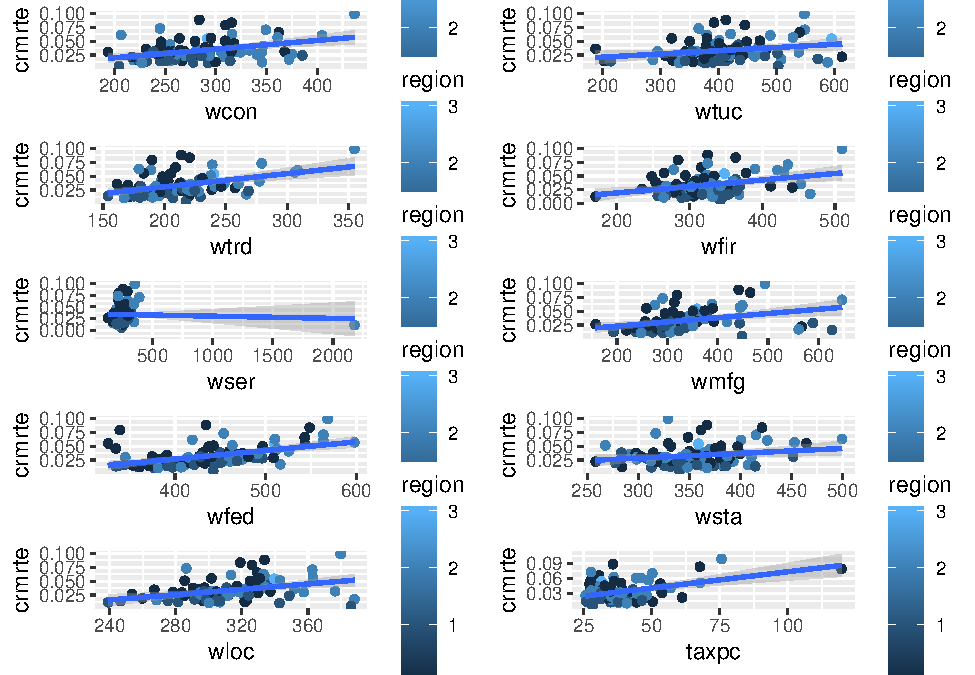
\includegraphics{Bagnard_Gaustad_Hartman_Leung_Lab_3_files/figure-latex/unnamed-chunk-18-1.pdf}

We observe a few data points of interest in the comparison above,
notably, wser appears to have an extreme data point.

Other variables show outliers as well, but not as extreme. We will
determine if any of these points have leverage or influence during model
specification.

For now, lets dig deeper into one of the extreme outliers after our
visual inspection.

\begin{Shaded}
\begin{Highlighting}[]
\NormalTok{dfCrime }\OperatorTok
\KeywordTok{filter}\NormalTok{(wser }\OperatorTok{>}\StringTok{ }\DecValTok{2000}\NormalTok{) }\OperatorTok
\KeywordTok{select}\NormalTok{(county, wser)}
\end{Highlighting}
\end{Shaded}

\begin{verbatim}
  county     wser
1    185 2177.068
\end{verbatim}

This average service wage is much too high based on what we know about
the 1980s and every other wage recorded in comparison. A review of the
detailed population statistics describing mean wage per industry (table
231) confirms this.
\url{https://www2.census.gov/prod2/decennial/documents/1980/1980censusofpopu801352uns_bw.pdf}

Outliers affect our ability to estimate statistics, resulting in
overestimated or underestimated values. Outliers can be due to a number
of different factors such as response errors and data entry errors.
Outliers will introduce bias into our estimates and are addressed during
the analysis phase. The mechanism for treatment include three approaches
1) trimming 2) winsorization or 3) imputation. Trimming will remove the
rest of the values in the observation and is not an preferred treatment.
Winsorazion relies on replacing outliers with the second largest or
second smallest value excluding the outlier. Imputation methods can use
the mean of a variable, or utilize regression models to predict the
missing value. A number of packages are available in R that use the
sample data to predict this value through regression. A full discussion
on treatment methods can be found here:
\url{http://www.asasrms.org/Proceedings/y2004/files/Jsm2004-000559.pdf}

We will use the Hmisc package which contains an impute function for
treatment of this outlier

\begin{Shaded}
\begin{Highlighting}[]
\NormalTok{dfCrime}\OperatorTok{$}\NormalTok{wser[}\KeywordTok{which}\NormalTok{(dfCrime}\OperatorTok{$}\NormalTok{county}\OperatorTok{==}\DecValTok{185}\NormalTok{)]<-}\OtherTok{NA} \CommentTok{# set the value to NA so it will be imputed}
\end{Highlighting}
\end{Shaded}

\begin{Shaded}
\begin{Highlighting}[]
\NormalTok{impute_arg <-}\StringTok{ }\KeywordTok{aregImpute}\NormalTok{(}\OperatorTok{~}\StringTok{ }\NormalTok{crmrte }\OperatorTok{+}\StringTok{  }\NormalTok{urban }\OperatorTok{+}\StringTok{ }\NormalTok{central }\OperatorTok{+}\StringTok{ }\NormalTok{west }\OperatorTok{+}\StringTok{ }\NormalTok{other }\OperatorTok{+}
\StringTok{                         }\NormalTok{prbarr }\OperatorTok{+}\StringTok{ }\NormalTok{prbconv }\OperatorTok{+}\StringTok{ }\NormalTok{prbpris }\OperatorTok{+}\StringTok{ }\NormalTok{avgsen }\OperatorTok{+}\StringTok{ }\NormalTok{polpc }\OperatorTok{+}\StringTok{ }
\StringTok{                         }\NormalTok{density }\OperatorTok{+}\StringTok{ }\NormalTok{taxpc }\OperatorTok{+}\StringTok{ }\NormalTok{pctmin80 }\OperatorTok{+}\StringTok{ }\NormalTok{wcon }\OperatorTok{+}\StringTok{ }\NormalTok{wtuc }\OperatorTok{+}
\StringTok{                         }\NormalTok{wtrd }\OperatorTok{+}\StringTok{ }\NormalTok{wfir }\OperatorTok{+}\StringTok{ }\NormalTok{wser }\OperatorTok{+}\StringTok{ }\NormalTok{wmfg }\OperatorTok{+}\StringTok{ }\NormalTok{wfed }\OperatorTok{+}\StringTok{ }\NormalTok{wsta }\OperatorTok{+}\StringTok{ }\NormalTok{wloc }\OperatorTok{+}
\StringTok{                         }\NormalTok{mix }\OperatorTok{+}\StringTok{ }\NormalTok{pctymle, }\DataTypeTok{data =}\NormalTok{ dfCrime, }\DataTypeTok{match=}\StringTok{"weighted"}\NormalTok{,}
                         \DataTypeTok{nk=}\DecValTok{3}\NormalTok{, }\DataTypeTok{B=}\DecValTok{10}\NormalTok{, }\DataTypeTok{n.impute =} \DecValTok{100}\NormalTok{)}
\end{Highlighting}
\end{Shaded}

\begin{Shaded}
\begin{Highlighting}[]
\KeywordTok{paste}\NormalTok{(}\StringTok{"R-squares for Predicting Non-Missing Values for Each Variable"}\NormalTok{)}
\end{Highlighting}
\end{Shaded}

\begin{verbatim}
[1] "R-squares for Predicting Non-Missing Values for Each Variable"
\end{verbatim}

\begin{Shaded}
\begin{Highlighting}[]
\NormalTok{impute_arg}\OperatorTok{$}\NormalTok{rsq}
\end{Highlighting}
\end{Shaded}

\begin{verbatim}
    wser 
0.841456 
\end{verbatim}

\begin{Shaded}
\begin{Highlighting}[]
\KeywordTok{paste}\NormalTok{(}\StringTok{"Distribution of Values for Each Imputation"}\NormalTok{)}
\end{Highlighting}
\end{Shaded}

\begin{verbatim}
[1] "Distribution of Values for Each Imputation"
\end{verbatim}

\begin{Shaded}
\begin{Highlighting}[]
\KeywordTok{table}\NormalTok{(impute_arg}\OperatorTok{$}\NormalTok{imputed}\OperatorTok{$}\NormalTok{wser)}
\end{Highlighting}
\end{Shaded}

\begin{verbatim}

133.0430603 172.4732666 172.6280975 192.3076935  206.281601 212.8205109 
          7           3           6           1           1           1 
213.5821533 230.4980621 238.4958496 242.4604797 245.2060852 247.6290894 
          2           2           1           1           1           1 
        250 253.2280579 266.0934143 274.1774597 274.8685913 295.9351501 
          1           1           1          64           1           1 
296.8684387 305.1542664 318.3635254  391.308075 
          1           1           1           1 
\end{verbatim}

We will reassign the value in our dataset to the mean from these trials.

\begin{Shaded}
\begin{Highlighting}[]
\NormalTok{dfCrime}\OperatorTok{$}\NormalTok{wser[}\KeywordTok{which}\NormalTok{(dfCrime}\OperatorTok{$}\NormalTok{county}\OperatorTok{==}\DecValTok{185}\NormalTok{)]<-}\KeywordTok{mean}\NormalTok{(impute_arg}\OperatorTok{$}\NormalTok{imputed}\OperatorTok{$}\NormalTok{wser)}
\NormalTok{dfCrime}\OperatorTok{$}\NormalTok{wser[}\KeywordTok{which}\NormalTok{(dfCrime}\OperatorTok{$}\NormalTok{county}\OperatorTok{==}\DecValTok{185}\NormalTok{)]}
\end{Highlighting}
\end{Shaded}

\begin{verbatim}
[1] 251.5703
\end{verbatim}

Next, we will examine the criminal justice variables.

\begin{Shaded}
\begin{Highlighting}[]
\CommentTok{#Plot of the criminal justice and law enforcment related variables vs crmrte}
\NormalTok{q1<-}\KeywordTok{ggplot}\NormalTok{(}\DataTypeTok{data =}\NormalTok{ dfCrime, }\KeywordTok{aes}\NormalTok{(}\DataTypeTok{x =}\NormalTok{ prbarr, }\DataTypeTok{y =}\NormalTok{ crmrte, }\DataTypeTok{color =}\NormalTok{ region)) }\OperatorTok{+}\StringTok{ }
\StringTok{      }\KeywordTok{geom_point}\NormalTok{()}\OperatorTok{+}
\StringTok{  }\KeywordTok{geom_smooth}\NormalTok{(}\DataTypeTok{method =} \StringTok{"lm"}\NormalTok{)}
\NormalTok{q2<-}\KeywordTok{ggplot}\NormalTok{(}\DataTypeTok{data =}\NormalTok{ dfCrime, }\KeywordTok{aes}\NormalTok{(}\DataTypeTok{x =}\NormalTok{ prbconv, }\DataTypeTok{y =}\NormalTok{ crmrte, }\DataTypeTok{color =}\NormalTok{ region)) }\OperatorTok{+}\StringTok{ }
\StringTok{      }\KeywordTok{geom_point}\NormalTok{()}\OperatorTok{+}
\StringTok{  }\KeywordTok{geom_smooth}\NormalTok{(}\DataTypeTok{method =} \StringTok{"lm"}\NormalTok{)}
\NormalTok{q3<-}\KeywordTok{ggplot}\NormalTok{(}\DataTypeTok{data =}\NormalTok{ dfCrime, }\KeywordTok{aes}\NormalTok{(}\DataTypeTok{x =}\NormalTok{ prbpris, }\DataTypeTok{y =}\NormalTok{ crmrte, }\DataTypeTok{color =}\NormalTok{ region)) }\OperatorTok{+}\StringTok{ }
\StringTok{      }\KeywordTok{geom_point}\NormalTok{()}\OperatorTok{+}
\StringTok{  }\KeywordTok{geom_smooth}\NormalTok{(}\DataTypeTok{method =} \StringTok{"lm"}\NormalTok{)}
\NormalTok{q4<-}\KeywordTok{ggplot}\NormalTok{(}\DataTypeTok{data =}\NormalTok{ dfCrime, }\KeywordTok{aes}\NormalTok{(}\DataTypeTok{x =}\NormalTok{ avgsen, }\DataTypeTok{y =}\NormalTok{ crmrte, }\DataTypeTok{color =}\NormalTok{ region)) }\OperatorTok{+}\StringTok{ }
\StringTok{      }\KeywordTok{geom_point}\NormalTok{()}\OperatorTok{+}
\StringTok{  }\KeywordTok{geom_smooth}\NormalTok{(}\DataTypeTok{method =} \StringTok{"lm"}\NormalTok{)}
\NormalTok{q5<-}\KeywordTok{ggplot}\NormalTok{(}\DataTypeTok{data =}\NormalTok{ dfCrime, }\KeywordTok{aes}\NormalTok{(}\DataTypeTok{x =}\NormalTok{ polpc, }\DataTypeTok{y =}\NormalTok{ crmrte, }\DataTypeTok{color =}\NormalTok{ region)) }\OperatorTok{+}\StringTok{ }
\StringTok{      }\KeywordTok{geom_point}\NormalTok{()}\OperatorTok{+}
\StringTok{  }\KeywordTok{geom_smooth}\NormalTok{(}\DataTypeTok{method =} \StringTok{"lm"}\NormalTok{)}
\NormalTok{q6<-}\KeywordTok{ggplot}\NormalTok{(}\DataTypeTok{data =}\NormalTok{ dfCrime, }\KeywordTok{aes}\NormalTok{(}\DataTypeTok{x =}\NormalTok{ mix, }\DataTypeTok{y =}\NormalTok{ crmrte, }\DataTypeTok{color =}\NormalTok{ region)) }\OperatorTok{+}\StringTok{ }
\StringTok{      }\KeywordTok{geom_point}\NormalTok{()}\OperatorTok{+}
\StringTok{  }\KeywordTok{geom_smooth}\NormalTok{(}\DataTypeTok{method =} \StringTok{"lm"}\NormalTok{)}

\KeywordTok{grid.arrange}\NormalTok{(q1, q2, q3, q4, q5, q6, }\DataTypeTok{ncol=}\DecValTok{2}\NormalTok{)}
\end{Highlighting}
\end{Shaded}

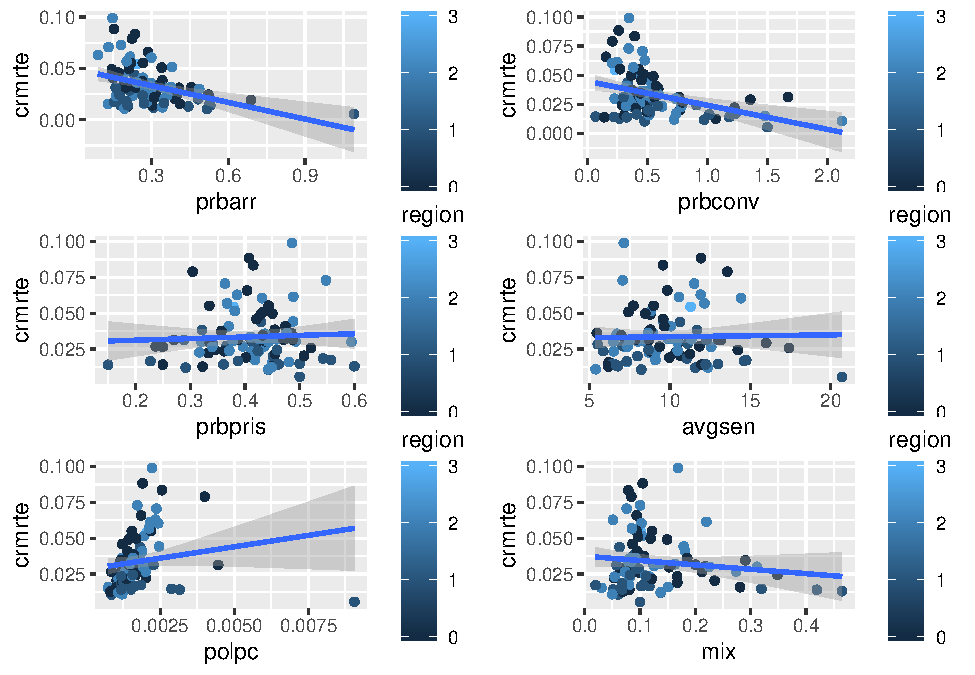
\includegraphics{Bagnard_Gaustad_Hartman_Leung_Lab_3_files/figure-latex/unnamed-chunk-25-1.pdf}

The criminal justice and law enforcement variables also show evidence of
possible outliers, notably, pbarr and polpc appear to have extreme data
points

We also see that prbarr and prbconv have values greater than 1. However,
these are not true probabity numbers and are instead ratios used as a
stand in for the true probability numbers.

There is a possibility of higher arrests per incident for an area.
Meaning, the area has low incidents in general but when there were
incidents there were also multiple arrests. The same case can be made
for the convictions per arrest variable which we see is for a different
region. In that county there may have been multiple charges brought per
one arrest.

\begin{Shaded}
\begin{Highlighting}[]
\CommentTok{#plot of demographic information for counties Outside and Inside the metro areas}
\CommentTok{# population density, percent minority, percent young male}

\NormalTok{q1<-}\KeywordTok{ggplot}\NormalTok{(}\DataTypeTok{data =}\NormalTok{ dfCrime, }\KeywordTok{aes}\NormalTok{(}\DataTypeTok{x =}\NormalTok{ density, }\DataTypeTok{y =}\NormalTok{ crmrte, }\DataTypeTok{color =}\NormalTok{ region)) }\OperatorTok{+}\StringTok{ }
\StringTok{      }\KeywordTok{geom_point}\NormalTok{() }\OperatorTok{+}\StringTok{ }\KeywordTok{facet_wrap}\NormalTok{(}\OperatorTok{~}\StringTok{ }\NormalTok{metro) }\OperatorTok{+}
\StringTok{  }\KeywordTok{geom_smooth}\NormalTok{(}\DataTypeTok{method =} \StringTok{"lm"}\NormalTok{)}
\NormalTok{q2<-}\KeywordTok{ggplot}\NormalTok{(}\DataTypeTok{data =}\NormalTok{ dfCrime, }\KeywordTok{aes}\NormalTok{(}\DataTypeTok{x =}\NormalTok{ pctmin80, }\DataTypeTok{y =}\NormalTok{ crmrte, }\DataTypeTok{color =}\NormalTok{ region)) }\OperatorTok{+}\StringTok{ }
\StringTok{      }\KeywordTok{geom_point}\NormalTok{() }\OperatorTok{+}\StringTok{ }\KeywordTok{facet_wrap}\NormalTok{(}\OperatorTok{~}\StringTok{ }\NormalTok{metro) }\OperatorTok{+}
\StringTok{  }\KeywordTok{geom_smooth}\NormalTok{(}\DataTypeTok{method =} \StringTok{"lm"}\NormalTok{)}
\NormalTok{q3<-}\KeywordTok{ggplot}\NormalTok{(}\DataTypeTok{data =}\NormalTok{ dfCrime, }\KeywordTok{aes}\NormalTok{(}\DataTypeTok{x =}\NormalTok{ pctymle, }\DataTypeTok{y =}\NormalTok{ crmrte, }\DataTypeTok{color =}\NormalTok{ region)) }\OperatorTok{+}\StringTok{ }
\StringTok{      }\KeywordTok{geom_point}\NormalTok{()}\OperatorTok{+}\StringTok{ }\KeywordTok{facet_wrap}\NormalTok{(}\OperatorTok{~}\StringTok{ }\NormalTok{metro) }\OperatorTok{+}
\StringTok{  }\KeywordTok{geom_smooth}\NormalTok{(}\DataTypeTok{method =} \StringTok{"lm"}\NormalTok{)}

\KeywordTok{grid.arrange}\NormalTok{(q1, q2, q3, }\DataTypeTok{ncol=}\DecValTok{1}\NormalTok{)}
\end{Highlighting}
\end{Shaded}

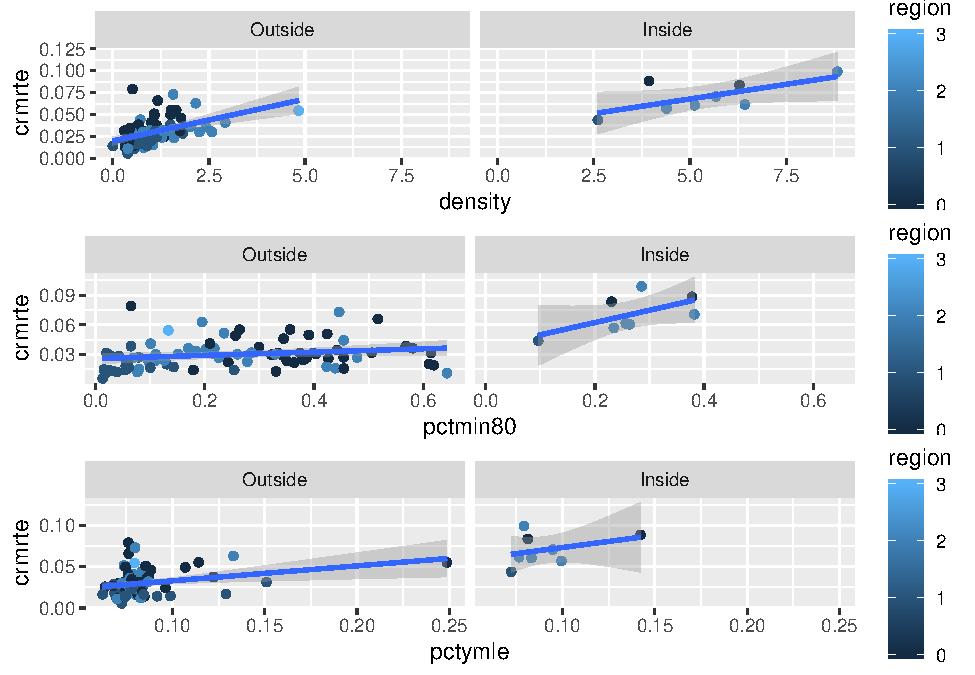
\includegraphics{Bagnard_Gaustad_Hartman_Leung_Lab_3_files/figure-latex/unnamed-chunk-26-1.pdf}

Notably more outliers are observed in demographic information. Here,
pctymle in one county outside of a metro area is nearly 25\%. That seems
quite high in normal statistical measures of the population, however,
this can be explained as a county having a large college town
population.

Finally, we can see our bright blue region 3 county and notice its
population density. Its behavior is more similar to an inside metro area
than outside. In addition to be coded for both western and central
regions, it appears to be miscoded here as well.

We will address the metro variable, and examine whether the region
variable should be west, central or other instead of both central and
west

\begin{Shaded}
\begin{Highlighting}[]
\NormalTok{dfCrime }\OperatorTok
\KeywordTok{filter}\NormalTok{(west }\OperatorTok{==}\DecValTok{1} \OperatorTok{&}\StringTok{ }\NormalTok{central }\OperatorTok{==}\DecValTok{1}\NormalTok{) }\OperatorTok
\KeywordTok{select}\NormalTok{(county, west, central, other, urban, region, regcode, metro)}
\end{Highlighting}
\end{Shaded}

\begin{verbatim}
  county west central other urban region regcode   metro
1     71    1       1     0     0      3      CW Outside
\end{verbatim}

\begin{Shaded}
\begin{Highlighting}[]
\NormalTok{dfCrime}\OperatorTok{$}\NormalTok{west[}\KeywordTok{which}\NormalTok{(dfCrime}\OperatorTok{$}\NormalTok{county}\OperatorTok{==}\DecValTok{71}\NormalTok{)]<-}\OtherTok{NA}
\NormalTok{dfCrime}\OperatorTok{$}\NormalTok{central[}\KeywordTok{which}\NormalTok{(dfCrime}\OperatorTok{$}\NormalTok{county}\OperatorTok{==}\DecValTok{71}\NormalTok{)]<-}\OtherTok{NA}
\NormalTok{dfCrime}\OperatorTok{$}\NormalTok{other[}\KeywordTok{which}\NormalTok{(dfCrime}\OperatorTok{$}\NormalTok{county}\OperatorTok{==}\DecValTok{71}\NormalTok{)]<-}\OtherTok{NA}
\NormalTok{dfCrime}\OperatorTok{$}\NormalTok{urban[}\KeywordTok{which}\NormalTok{(dfCrime}\OperatorTok{$}\NormalTok{county}\OperatorTok{==}\DecValTok{71}\NormalTok{)]<-}\OtherTok{NA}
\end{Highlighting}
\end{Shaded}

\begin{Shaded}
\begin{Highlighting}[]
\NormalTok{impute_arg <-}\StringTok{ }\KeywordTok{aregImpute}\NormalTok{(}\OperatorTok{~}\StringTok{ }\NormalTok{crmrte }\OperatorTok{+}\StringTok{  }\NormalTok{urban }\OperatorTok{+}\StringTok{ }\NormalTok{central }\OperatorTok{+}\StringTok{ }\NormalTok{west }\OperatorTok{+}
\StringTok{                         }\NormalTok{prbarr }\OperatorTok{+}\StringTok{ }\NormalTok{prbconv }\OperatorTok{+}\StringTok{ }\NormalTok{prbpris }\OperatorTok{+}\StringTok{ }\NormalTok{avgsen }\OperatorTok{+}\StringTok{ }\NormalTok{polpc }\OperatorTok{+}\StringTok{ }
\StringTok{                         }\NormalTok{density }\OperatorTok{+}\StringTok{ }\NormalTok{taxpc }\OperatorTok{+}\StringTok{ }\NormalTok{pctmin80 }\OperatorTok{+}\StringTok{ }\NormalTok{wcon }\OperatorTok{+}\StringTok{ }\NormalTok{wtuc }\OperatorTok{+}
\StringTok{                         }\NormalTok{wtrd }\OperatorTok{+}\StringTok{ }\NormalTok{wfir }\OperatorTok{+}\StringTok{ }\NormalTok{wser }\OperatorTok{+}\StringTok{ }\NormalTok{wmfg }\OperatorTok{+}\StringTok{ }\NormalTok{wfed }\OperatorTok{+}\StringTok{ }\NormalTok{wsta }\OperatorTok{+}\StringTok{ }\NormalTok{wloc }\OperatorTok{+}
\StringTok{                         }\NormalTok{mix }\OperatorTok{+}\StringTok{ }\NormalTok{pctymle, }\DataTypeTok{data =}\NormalTok{ dfCrime, }\DataTypeTok{match=}\StringTok{"weighted"}\NormalTok{,}
                         \DataTypeTok{nk=}\DecValTok{3}\NormalTok{, }\DataTypeTok{B=}\DecValTok{10}\NormalTok{, }\DataTypeTok{n.impute =} \DecValTok{100}\NormalTok{)}
\end{Highlighting}
\end{Shaded}

\begin{Shaded}
\begin{Highlighting}[]
\KeywordTok{paste}\NormalTok{(}\StringTok{"R-squares for Predicting Non-Missing Values for Each Variable"}\NormalTok{)}
\end{Highlighting}
\end{Shaded}

\begin{verbatim}
[1] "R-squares for Predicting Non-Missing Values for Each Variable"
\end{verbatim}

\begin{Shaded}
\begin{Highlighting}[]
\NormalTok{impute_arg}\OperatorTok{$}\NormalTok{rsq}
\end{Highlighting}
\end{Shaded}

\begin{verbatim}
    urban   central      west 
0.9739368 0.8905421 0.9205110 
\end{verbatim}

\begin{Shaded}
\begin{Highlighting}[]
\KeywordTok{paste}\NormalTok{(}\StringTok{"Distribution of Values for Each Imputation"}\NormalTok{)}
\end{Highlighting}
\end{Shaded}

\begin{verbatim}
[1] "Distribution of Values for Each Imputation"
\end{verbatim}

\begin{Shaded}
\begin{Highlighting}[]
\KeywordTok{table}\NormalTok{(impute_arg}\OperatorTok{$}\NormalTok{imputed}\OperatorTok{$}\NormalTok{central)}
\end{Highlighting}
\end{Shaded}

\begin{verbatim}

 0  1 
42 58 
\end{verbatim}

\begin{Shaded}
\begin{Highlighting}[]
\KeywordTok{paste}\NormalTok{(}\StringTok{"Distribution of Values for Each Imputation"}\NormalTok{)}
\end{Highlighting}
\end{Shaded}

\begin{verbatim}
[1] "Distribution of Values for Each Imputation"
\end{verbatim}

\begin{Shaded}
\begin{Highlighting}[]
\KeywordTok{table}\NormalTok{(impute_arg}\OperatorTok{$}\NormalTok{imputed}\OperatorTok{$}\NormalTok{west)}
\end{Highlighting}
\end{Shaded}

\begin{verbatim}

 0  1 
81 19 
\end{verbatim}

\begin{Shaded}
\begin{Highlighting}[]
\KeywordTok{paste}\NormalTok{(}\StringTok{"Distribution of Values for Each Imputation"}\NormalTok{)}
\end{Highlighting}
\end{Shaded}

\begin{verbatim}
[1] "Distribution of Values for Each Imputation"
\end{verbatim}

\begin{Shaded}
\begin{Highlighting}[]
\KeywordTok{table}\NormalTok{(impute_arg}\OperatorTok{$}\NormalTok{imputed}\OperatorTok{$}\NormalTok{urban)}
\end{Highlighting}
\end{Shaded}

\begin{verbatim}

 0  1 
13 87 
\end{verbatim}

The results confirm the county is urban. It is also highly probable that
county 71 is not west and most likely associated with central. After
correcting our data for urban and west, let's compare `central' with
`other' to be certain we have the right region.

\begin{Shaded}
\begin{Highlighting}[]
\CommentTok{#We need a mode function, so lets define one. Source - public domain}
\NormalTok{Mode =}\StringTok{ }\ControlFlowTok{function}\NormalTok{(x)\{ }
\NormalTok{    ta =}\StringTok{ }\KeywordTok{table}\NormalTok{(x)}
\NormalTok{    tam =}\StringTok{ }\KeywordTok{max}\NormalTok{(ta)}
    \ControlFlowTok{if}\NormalTok{ (}\KeywordTok{all}\NormalTok{(ta }\OperatorTok{==}\StringTok{ }\NormalTok{tam))}
\NormalTok{         mod =}\StringTok{ }\OtherTok{NA}
    \ControlFlowTok{else}
         \ControlFlowTok{if}\NormalTok{(}\KeywordTok{is.numeric}\NormalTok{(x))}
\NormalTok{    mod =}\StringTok{ }\KeywordTok{as.numeric}\NormalTok{(}\KeywordTok{names}\NormalTok{(ta)[ta }\OperatorTok{==}\StringTok{ }\NormalTok{tam])}
    \ControlFlowTok{else}
\NormalTok{         mod =}\StringTok{ }\KeywordTok{names}\NormalTok{(ta)[ta }\OperatorTok{==}\StringTok{ }\NormalTok{tam]}
    \KeywordTok{return}\NormalTok{(mod)}
\NormalTok{\}}

\NormalTok{dfCrime}\OperatorTok{$}\NormalTok{urban[}\KeywordTok{which}\NormalTok{(dfCrime}\OperatorTok{$}\NormalTok{county}\OperatorTok{==}\DecValTok{71}\NormalTok{)]<-}\KeywordTok{Mode}\NormalTok{(impute_arg}\OperatorTok{$}\NormalTok{imputed}\OperatorTok{$}\NormalTok{urban)}
\NormalTok{dfCrime}\OperatorTok{$}\NormalTok{urban[}\KeywordTok{which}\NormalTok{(dfCrime}\OperatorTok{$}\NormalTok{county}\OperatorTok{==}\DecValTok{71}\NormalTok{)]}
\end{Highlighting}
\end{Shaded}

\begin{verbatim}
[1] 1
\end{verbatim}

\begin{Shaded}
\begin{Highlighting}[]
\NormalTok{dfCrime}\OperatorTok{$}\NormalTok{nonurban[}\KeywordTok{which}\NormalTok{(dfCrime}\OperatorTok{$}\NormalTok{county}\OperatorTok{==}\DecValTok{71}\NormalTok{)]<-}\DecValTok{1}\OperatorTok{-}\KeywordTok{Mode}\NormalTok{(impute_arg}\OperatorTok{$}\NormalTok{imputed}\OperatorTok{$}\NormalTok{urban)}
\NormalTok{dfCrime}\OperatorTok{$}\NormalTok{nonurban[}\KeywordTok{which}\NormalTok{(dfCrime}\OperatorTok{$}\NormalTok{county}\OperatorTok{==}\DecValTok{71}\NormalTok{)]}
\end{Highlighting}
\end{Shaded}

\begin{verbatim}
[1] 0
\end{verbatim}

\begin{Shaded}
\begin{Highlighting}[]
\NormalTok{dfCrime}\OperatorTok{$}\NormalTok{west[}\KeywordTok{which}\NormalTok{(dfCrime}\OperatorTok{$}\NormalTok{county}\OperatorTok{==}\DecValTok{71}\NormalTok{)]<-}\KeywordTok{Mode}\NormalTok{(impute_arg}\OperatorTok{$}\NormalTok{imputed}\OperatorTok{$}\NormalTok{west)}
\NormalTok{dfCrime}\OperatorTok{$}\NormalTok{west[}\KeywordTok{which}\NormalTok{(dfCrime}\OperatorTok{$}\NormalTok{county}\OperatorTok{==}\DecValTok{71}\NormalTok{)]}
\end{Highlighting}
\end{Shaded}

\begin{verbatim}
[1] 0
\end{verbatim}

\begin{Shaded}
\begin{Highlighting}[]
\NormalTok{impute_arg <-}\StringTok{ }\KeywordTok{aregImpute}\NormalTok{(}\OperatorTok{~}\StringTok{ }\NormalTok{crmrte }\OperatorTok{+}\StringTok{ }\NormalTok{central }\OperatorTok{+}\StringTok{ }\NormalTok{other }\OperatorTok{+}
\StringTok{                         }\NormalTok{prbarr }\OperatorTok{+}\StringTok{ }\NormalTok{prbconv }\OperatorTok{+}\StringTok{ }\NormalTok{prbpris }\OperatorTok{+}\StringTok{ }\NormalTok{avgsen }\OperatorTok{+}\StringTok{ }\NormalTok{polpc }\OperatorTok{+}\StringTok{ }
\StringTok{                         }\NormalTok{density }\OperatorTok{+}\StringTok{ }\NormalTok{taxpc }\OperatorTok{+}\StringTok{ }\NormalTok{pctmin80 }\OperatorTok{+}\StringTok{ }\NormalTok{wcon }\OperatorTok{+}\StringTok{ }\NormalTok{wtuc }\OperatorTok{+}
\StringTok{                         }\NormalTok{wtrd }\OperatorTok{+}\StringTok{ }\NormalTok{wfir }\OperatorTok{+}\StringTok{ }\NormalTok{wser }\OperatorTok{+}\StringTok{ }\NormalTok{wmfg }\OperatorTok{+}\StringTok{ }\NormalTok{wfed }\OperatorTok{+}\StringTok{ }\NormalTok{wsta }\OperatorTok{+}\StringTok{ }\NormalTok{wloc }\OperatorTok{+}
\StringTok{                         }\NormalTok{mix }\OperatorTok{+}\StringTok{ }\NormalTok{pctymle, }\DataTypeTok{data =}\NormalTok{ dfCrime, }\DataTypeTok{match=}\StringTok{"weighted"}\NormalTok{,}
                         \DataTypeTok{nk=}\DecValTok{3}\NormalTok{, }\DataTypeTok{B=}\DecValTok{10}\NormalTok{, }\DataTypeTok{n.impute =} \DecValTok{100}\NormalTok{)}
\end{Highlighting}
\end{Shaded}

\begin{Shaded}
\begin{Highlighting}[]
\KeywordTok{paste}\NormalTok{(}\StringTok{"R-squares for Predicting Non-Missing Values for Each Variable"}\NormalTok{)}
\end{Highlighting}
\end{Shaded}

\begin{verbatim}
[1] "R-squares for Predicting Non-Missing Values for Each Variable"
\end{verbatim}

\begin{Shaded}
\begin{Highlighting}[]
\NormalTok{impute_arg}\OperatorTok{$}\NormalTok{rsq}
\end{Highlighting}
\end{Shaded}

\begin{verbatim}
  central     other 
0.9479975 0.9349436 
\end{verbatim}

\begin{Shaded}
\begin{Highlighting}[]
\KeywordTok{paste}\NormalTok{(}\StringTok{"Distribution of Values for Each Imputation"}\NormalTok{)}
\end{Highlighting}
\end{Shaded}

\begin{verbatim}
[1] "Distribution of Values for Each Imputation"
\end{verbatim}

\begin{Shaded}
\begin{Highlighting}[]
\KeywordTok{table}\NormalTok{(impute_arg}\OperatorTok{$}\NormalTok{imputed}\OperatorTok{$}\NormalTok{other)}
\end{Highlighting}
\end{Shaded}

\begin{verbatim}

 0  1 
83 17 
\end{verbatim}

\begin{Shaded}
\begin{Highlighting}[]
\KeywordTok{paste}\NormalTok{(}\StringTok{"Distribution of Values for Each Imputation"}\NormalTok{)}
\end{Highlighting}
\end{Shaded}

\begin{verbatim}
[1] "Distribution of Values for Each Imputation"
\end{verbatim}

\begin{Shaded}
\begin{Highlighting}[]
\KeywordTok{table}\NormalTok{(impute_arg}\OperatorTok{$}\NormalTok{imputed}\OperatorTok{$}\NormalTok{central)}
\end{Highlighting}
\end{Shaded}

\begin{verbatim}

 0  1 
25 75 
\end{verbatim}

We also show a strong likelihood of the county not being other. The case
for central is high. Since the county is not western and not other it
must be in central by default, and the Hmisc algorithm bolsters that
suggestion. We'll assign our new values.

\begin{Shaded}
\begin{Highlighting}[]
\NormalTok{dfCrime}\OperatorTok{$}\NormalTok{other[}\KeywordTok{which}\NormalTok{(dfCrime}\OperatorTok{$}\NormalTok{county}\OperatorTok{==}\DecValTok{71}\NormalTok{)]<-}\KeywordTok{Mode}\NormalTok{(impute_arg}\OperatorTok{$}\NormalTok{imputed}\OperatorTok{$}\NormalTok{other)}
\NormalTok{dfCrime}\OperatorTok{$}\NormalTok{other[}\KeywordTok{which}\NormalTok{(dfCrime}\OperatorTok{$}\NormalTok{county}\OperatorTok{==}\DecValTok{71}\NormalTok{)]}
\end{Highlighting}
\end{Shaded}

\begin{verbatim}
[1] 0
\end{verbatim}

\begin{Shaded}
\begin{Highlighting}[]
\NormalTok{dfCrime}\OperatorTok{$}\NormalTok{central[}\KeywordTok{which}\NormalTok{(dfCrime}\OperatorTok{$}\NormalTok{county}\OperatorTok{==}\DecValTok{71}\NormalTok{)]<-}\DecValTok{1}\OperatorTok{-}\KeywordTok{Mode}\NormalTok{(impute_arg}\OperatorTok{$}\NormalTok{imputed}\OperatorTok{$}\NormalTok{other)}
\NormalTok{dfCrime}\OperatorTok{$}\NormalTok{central[}\KeywordTok{which}\NormalTok{(dfCrime}\OperatorTok{$}\NormalTok{county}\OperatorTok{==}\DecValTok{71}\NormalTok{)]}
\end{Highlighting}
\end{Shaded}

\begin{verbatim}
[1] 1
\end{verbatim}

Recode the categories for region and metro

\begin{Shaded}
\begin{Highlighting}[]
\NormalTok{dfCrime}\OperatorTok{$}\NormalTok{region <-}\StringTok{ }\KeywordTok{case_when}\NormalTok{ (}
\NormalTok{            (dfCrime}\OperatorTok{$}\NormalTok{central }\OperatorTok{==}\DecValTok{0} \OperatorTok{&}\StringTok{ }\NormalTok{dfCrime}\OperatorTok{$}\NormalTok{west }\OperatorTok{==}\DecValTok{0}\NormalTok{) }\OperatorTok{~}\StringTok{ }\DecValTok{0}\NormalTok{, }\CommentTok{#Eastern, Coastal, Other}
\NormalTok{            (dfCrime}\OperatorTok{$}\NormalTok{central }\OperatorTok{==}\DecValTok{0} \OperatorTok{&}\StringTok{ }\NormalTok{dfCrime}\OperatorTok{$}\NormalTok{west }\OperatorTok{==}\DecValTok{1}\NormalTok{) }\OperatorTok{~}\StringTok{ }\DecValTok{1}\NormalTok{, }\CommentTok{#Western}
\NormalTok{            (dfCrime}\OperatorTok{$}\NormalTok{central }\OperatorTok{==}\DecValTok{1} \OperatorTok{&}\StringTok{ }\NormalTok{dfCrime}\OperatorTok{$}\NormalTok{west }\OperatorTok{==}\DecValTok{0}\NormalTok{) }\OperatorTok{~}\StringTok{ }\DecValTok{2}  \CommentTok{#Central}
\NormalTok{        )}
\NormalTok{dfCrime}\OperatorTok{$}\NormalTok{regcode =}
\StringTok{            }\KeywordTok{factor}\NormalTok{( dfCrime}\OperatorTok{$}\NormalTok{region , }\DataTypeTok{levels =} \DecValTok{0}\OperatorTok{:}\DecValTok{2}\NormalTok{ , }\DataTypeTok{labels =}
                    \KeywordTok{c}\NormalTok{( }\StringTok{'O'}\NormalTok{,}
                       \StringTok{'W'}\NormalTok{,}
                       \StringTok{'C'}\NormalTok{ )}
\NormalTok{                   )}
\end{Highlighting}
\end{Shaded}

\begin{Shaded}
\begin{Highlighting}[]
\NormalTok{dfCrime}\OperatorTok{$}\NormalTok{metro =}
\StringTok{            }\KeywordTok{factor}\NormalTok{( dfCrime}\OperatorTok{$}\NormalTok{urban , }\DataTypeTok{levels =} \DecValTok{0}\OperatorTok{:}\DecValTok{1}\NormalTok{ , }\DataTypeTok{labels =}
                    \KeywordTok{c}\NormalTok{( }\StringTok{'Outside'}\NormalTok{,}
                       \StringTok{'Inside'}
\NormalTok{                      )}
\NormalTok{                   )}
\end{Highlighting}
\end{Shaded}

\begin{Shaded}
\begin{Highlighting}[]
\NormalTok{dfCrime }\OperatorTok
\KeywordTok{filter}\NormalTok{(county }\OperatorTok{==}\StringTok{ }\DecValTok{71}\NormalTok{) }\OperatorTok
\KeywordTok{select}\NormalTok{(county, west, central, urban, region, regcode, metro)}
\end{Highlighting}
\end{Shaded}

\begin{verbatim}
  county west central urban region regcode  metro
1     71    0       1     1      2       C Inside
\end{verbatim}

Let's review our density numbers again by looking in more detail at its
distribution.

\begin{Shaded}
\begin{Highlighting}[]
\KeywordTok{options}\NormalTok{(}\DataTypeTok{repr.plot.width=}\DecValTok{8}\NormalTok{, }\DataTypeTok{repr.plot.height=}\DecValTok{4}\NormalTok{)}
\KeywordTok{ggplot}\NormalTok{(}\DataTypeTok{data =}\NormalTok{ dfCrime, }\KeywordTok{aes}\NormalTok{(}\DataTypeTok{x =}\NormalTok{ density)) }\OperatorTok{+}\StringTok{ }
\StringTok{      }\KeywordTok{geom_histogram}\NormalTok{(}\DataTypeTok{bins=}\DecValTok{90}\NormalTok{)}
\end{Highlighting}
\end{Shaded}

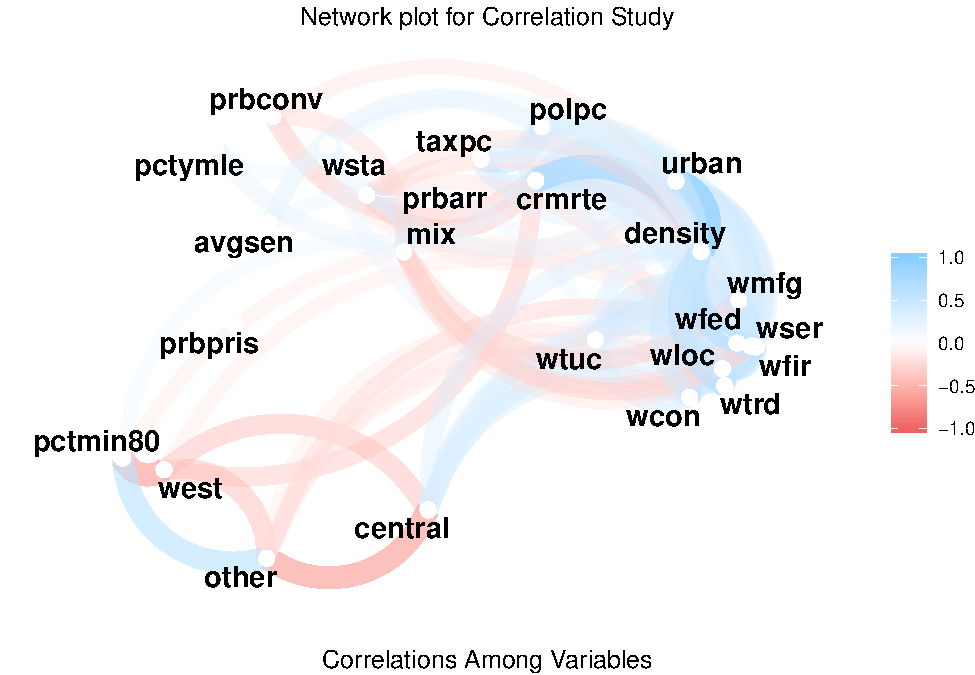
\includegraphics{Bagnard_Gaustad_Hartman_Leung_Lab_3_files/figure-latex/unnamed-chunk-43-1.pdf}

We note that one of the counties has an extremely low density. Near
zero.

\begin{Shaded}
\begin{Highlighting}[]
\NormalTok{dfCrime }\OperatorTok
\KeywordTok{filter}\NormalTok{(density }\OperatorTok{<}\StringTok{ }\FloatTok{0.01}\NormalTok{)}
\end{Highlighting}
\end{Shaded}

\begin{verbatim}
  county year    crmrte   prbarr  prbconv prbpris avgsen      polpc
1    173   87 0.0139937 0.530435 0.327869    0.15   6.64 0.00316379
      density    taxpc west central urban pctmin80    wcon     wtuc
1 2.03422e-05 37.72702    1       0     0 0.253914 231.696 213.6752
      wtrd    wfir     wser   wmfg   wfed   wsta   wloc       mix
1 175.1604 267.094 204.3792 193.01 334.44 414.68 304.32 0.4197531
     pctymle region regcode other nonurban   metro
1 0.07462687      1       W     0        1 Outside
\end{verbatim}

In review of the North Carolina county density data from 1985, the
smallest population density in any county in North Carolina is 0.0952.
This makes the density of 0.0000203422 for county 173 statistically
impossible. It is miscoded.

\url{http://ncosbm.s3.amazonaws.com/s3fs-public/demog/dens7095.xls}

(Note to team: We could use this table if we want to assign names to our
counties by comparing the population densities. What is interesting is
that the 6 rows of missing values we removed earlier can be found in the
tail of this table. There was an arbitrary cut off after a certain
density - lkely because the counties were not statistically significant.
County 173 is not one of those counties, however, as our imputation
process will demonstrate.)

\begin{Shaded}
\begin{Highlighting}[]
\NormalTok{dfCrime}\OperatorTok{$}\NormalTok{density[}\KeywordTok{which}\NormalTok{(dfCrime}\OperatorTok{$}\NormalTok{county}\OperatorTok{==}\DecValTok{173}\NormalTok{)]<-}\StringTok{ }\OtherTok{NA}
\end{Highlighting}
\end{Shaded}

\begin{Shaded}
\begin{Highlighting}[]
\CommentTok{#dfSubset <-  we will use the non-urban western counties}
\NormalTok{impute_arg <-}\StringTok{ }\KeywordTok{aregImpute}\NormalTok{(}\OperatorTok{~}\StringTok{ }\NormalTok{crmrte }\OperatorTok{+}\StringTok{ }
\StringTok{                         }\NormalTok{prbarr }\OperatorTok{+}\StringTok{ }\NormalTok{prbconv }\OperatorTok{+}\StringTok{ }\NormalTok{prbpris }\OperatorTok{+}\StringTok{ }\NormalTok{avgsen }\OperatorTok{+}\StringTok{ }\NormalTok{polpc }\OperatorTok{+}\StringTok{ }
\StringTok{                         }\NormalTok{density }\OperatorTok{+}\StringTok{ }\NormalTok{taxpc }\OperatorTok{+}\StringTok{ }\NormalTok{pctmin80 }\OperatorTok{+}\StringTok{ }\NormalTok{wcon }\OperatorTok{+}\StringTok{ }\NormalTok{wtuc }\OperatorTok{+}
\StringTok{                         }\NormalTok{wtrd }\OperatorTok{+}\StringTok{ }\NormalTok{wfir }\OperatorTok{+}\StringTok{ }\NormalTok{wser }\OperatorTok{+}\StringTok{ }\NormalTok{wmfg }\OperatorTok{+}\StringTok{ }\NormalTok{wfed }\OperatorTok{+}\StringTok{ }\NormalTok{wsta }\OperatorTok{+}\StringTok{ }\NormalTok{wloc }\OperatorTok{+}
\StringTok{                         }\NormalTok{mix }\OperatorTok{+}\StringTok{ }\NormalTok{pctymle, }\DataTypeTok{data =}\NormalTok{ dfCrime }\OperatorTok\StringTok{ }\KeywordTok{filter}\NormalTok{(urban}\OperatorTok{==}\DecValTok{0} \OperatorTok{&}\StringTok{ }\NormalTok{west }\OperatorTok{==}\DecValTok{1}\NormalTok{),}
                         \DataTypeTok{match=}\StringTok{"weighted"}\NormalTok{,  }\DataTypeTok{nk=}\DecValTok{3}\NormalTok{, }\DataTypeTok{B=}\DecValTok{10}\NormalTok{, }\DataTypeTok{n.impute =} \DecValTok{30}\NormalTok{)}
\end{Highlighting}
\end{Shaded}

\begin{Shaded}
\begin{Highlighting}[]
\KeywordTok{paste}\NormalTok{(}\StringTok{"R-squares for Predicting Non-Missing Values for Each Variable"}\NormalTok{)}
\end{Highlighting}
\end{Shaded}

\begin{verbatim}
[1] "R-squares for Predicting Non-Missing Values for Each Variable"
\end{verbatim}

\begin{Shaded}
\begin{Highlighting}[]
\NormalTok{impute_arg}\OperatorTok{$}\NormalTok{rsq}
\end{Highlighting}
\end{Shaded}

\begin{verbatim}
density 
      1 
\end{verbatim}

\begin{Shaded}
\begin{Highlighting}[]
\KeywordTok{paste}\NormalTok{(}\StringTok{"Distribution of Values for Each Imputation"}\NormalTok{)}
\end{Highlighting}
\end{Shaded}

\begin{verbatim}
[1] "Distribution of Values for Each Imputation"
\end{verbatim}

\begin{Shaded}
\begin{Highlighting}[]
\KeywordTok{table}\NormalTok{(impute_arg}\OperatorTok{$}\NormalTok{imputed}\OperatorTok{$}\NormalTok{density)}
\end{Highlighting}
\end{Shaded}

\begin{verbatim}

 0.41276595 0.687830687 0.889880955 1.815508008 
         26           1           2           1 
\end{verbatim}

\begin{Shaded}
\begin{Highlighting}[]
\NormalTok{dfCrime}\OperatorTok{$}\NormalTok{density[}\KeywordTok{which}\NormalTok{(dfCrime}\OperatorTok{$}\NormalTok{county}\OperatorTok{==}\DecValTok{173}\NormalTok{)]<-}\KeywordTok{mean}\NormalTok{(impute_arg}\OperatorTok{$}\NormalTok{imputed}\OperatorTok{$}\NormalTok{density)}
\NormalTok{dfCrime}\OperatorTok{$}\NormalTok{density[}\KeywordTok{which}\NormalTok{(dfCrime}\OperatorTok{$}\NormalTok{county}\OperatorTok{==}\DecValTok{173}\NormalTok{)]}
\end{Highlighting}
\end{Shaded}

\begin{verbatim}
[1] 0.5005005
\end{verbatim}

Now, we will examine transforms for better linearity.

\begin{Shaded}
\begin{Highlighting}[]
\CommentTok{#dfEconVars <- as.data.frame(cbind(dfCrime$wcon, dfCrime$wtuc, dfCrime$wtrd, dfCrime$wfir, }
\CommentTok{#                                  dfCrime$wser, dfCrime$wmfg, dfCrime$wfed, dfCrime$wsta, }
\CommentTok{#                                  dfCrime$wloc))}
\CommentTok{#names(dfEconVars) <- c('wcon', 'wtuc', 'wtrd', 'wfir', 'wser', }
\CommentTok{#                              'wmfg', 'wfed', 'wsta', 'wloc')}
\CommentTok{#}
\CommentTok{#ggplot(melt(dfEconVars),aes(x=value)) + geom_histogram(bins=30) + facet_wrap(~variable)}

\CommentTok{#The economic variables}
\NormalTok{q1<-}\KeywordTok{ggplot}\NormalTok{(}\DataTypeTok{data =}\NormalTok{ dfCrime, }\KeywordTok{aes}\NormalTok{(}\DataTypeTok{x =}\NormalTok{ wcon, }\DataTypeTok{y =}\NormalTok{ crmrte, }\DataTypeTok{color =}\NormalTok{ region)) }\OperatorTok{+}\StringTok{ }
\StringTok{      }\KeywordTok{geom_point}\NormalTok{()}\OperatorTok{+}
\StringTok{  }\KeywordTok{geom_smooth}\NormalTok{(}\DataTypeTok{method =} \StringTok{"lm"}\NormalTok{)}
\NormalTok{q1a<-}\KeywordTok{ggplot}\NormalTok{(}\DataTypeTok{data =}\NormalTok{ dfCrime, }\KeywordTok{aes}\NormalTok{(}\DataTypeTok{x =} \KeywordTok{log}\NormalTok{(wcon), }\DataTypeTok{y =} \KeywordTok{log}\NormalTok{(crmrte), }\DataTypeTok{color =}\NormalTok{ region)) }\OperatorTok{+}\StringTok{ }
\StringTok{      }\KeywordTok{geom_point}\NormalTok{()}\OperatorTok{+}
\StringTok{  }\KeywordTok{geom_smooth}\NormalTok{(}\DataTypeTok{method =} \StringTok{"lm"}\NormalTok{)}
\NormalTok{q2<-}\KeywordTok{ggplot}\NormalTok{(}\DataTypeTok{data =}\NormalTok{ dfCrime, }\KeywordTok{aes}\NormalTok{(}\DataTypeTok{x =}\NormalTok{ wtuc, }\DataTypeTok{y =}\NormalTok{ crmrte, }\DataTypeTok{color =}\NormalTok{ region)) }\OperatorTok{+}\StringTok{ }
\StringTok{      }\KeywordTok{geom_point}\NormalTok{()}\OperatorTok{+}
\StringTok{  }\KeywordTok{geom_smooth}\NormalTok{(}\DataTypeTok{method =} \StringTok{"lm"}\NormalTok{)}
\NormalTok{q2a<-}\KeywordTok{ggplot}\NormalTok{(}\DataTypeTok{data =}\NormalTok{ dfCrime, }\KeywordTok{aes}\NormalTok{(}\DataTypeTok{x =} \KeywordTok{log}\NormalTok{(wtuc), }\DataTypeTok{y =} \KeywordTok{log}\NormalTok{(crmrte), }\DataTypeTok{color =}\NormalTok{ region)) }\OperatorTok{+}\StringTok{ }
\StringTok{      }\KeywordTok{geom_point}\NormalTok{()}\OperatorTok{+}
\StringTok{  }\KeywordTok{geom_smooth}\NormalTok{(}\DataTypeTok{method =} \StringTok{"lm"}\NormalTok{)}
\NormalTok{q3<-}\KeywordTok{ggplot}\NormalTok{(}\DataTypeTok{data =}\NormalTok{ dfCrime, }\KeywordTok{aes}\NormalTok{(}\DataTypeTok{x =}\NormalTok{ wtrd, }\DataTypeTok{y =}\NormalTok{ crmrte, }\DataTypeTok{color =}\NormalTok{ region)) }\OperatorTok{+}\StringTok{ }
\StringTok{      }\KeywordTok{geom_point}\NormalTok{()}\OperatorTok{+}
\StringTok{  }\KeywordTok{geom_smooth}\NormalTok{(}\DataTypeTok{method =} \StringTok{"lm"}\NormalTok{)}
\NormalTok{q3a<-}\KeywordTok{ggplot}\NormalTok{(}\DataTypeTok{data =}\NormalTok{ dfCrime, }\KeywordTok{aes}\NormalTok{(}\DataTypeTok{x =} \KeywordTok{log}\NormalTok{(wtrd), }\DataTypeTok{y =} \KeywordTok{log}\NormalTok{(crmrte), }\DataTypeTok{color =}\NormalTok{ region)) }\OperatorTok{+}\StringTok{ }
\StringTok{      }\KeywordTok{geom_point}\NormalTok{()}\OperatorTok{+}
\StringTok{  }\KeywordTok{geom_smooth}\NormalTok{(}\DataTypeTok{method =} \StringTok{"lm"}\NormalTok{)}
\NormalTok{q4<-}\KeywordTok{ggplot}\NormalTok{(}\DataTypeTok{data =}\NormalTok{ dfCrime, }\KeywordTok{aes}\NormalTok{(}\DataTypeTok{x =}\NormalTok{ wfir, }\DataTypeTok{y =}\NormalTok{ crmrte, }\DataTypeTok{color =}\NormalTok{ region)) }\OperatorTok{+}\StringTok{ }
\StringTok{      }\KeywordTok{geom_point}\NormalTok{()}\OperatorTok{+}
\StringTok{  }\KeywordTok{geom_smooth}\NormalTok{(}\DataTypeTok{method =} \StringTok{"lm"}\NormalTok{)}
\NormalTok{q4a<-}\KeywordTok{ggplot}\NormalTok{(}\DataTypeTok{data =}\NormalTok{ dfCrime, }\KeywordTok{aes}\NormalTok{(}\DataTypeTok{x =} \KeywordTok{log}\NormalTok{(wfir), }\DataTypeTok{y =} \KeywordTok{log}\NormalTok{(crmrte), }\DataTypeTok{color =}\NormalTok{ region)) }\OperatorTok{+}\StringTok{ }
\StringTok{      }\KeywordTok{geom_point}\NormalTok{()}\OperatorTok{+}
\StringTok{  }\KeywordTok{geom_smooth}\NormalTok{(}\DataTypeTok{method =} \StringTok{"lm"}\NormalTok{)}
\NormalTok{q5<-}\KeywordTok{ggplot}\NormalTok{(}\DataTypeTok{data =}\NormalTok{ dfCrime, }\KeywordTok{aes}\NormalTok{(}\DataTypeTok{x =}\NormalTok{ wser, }\DataTypeTok{y =}\NormalTok{ crmrte, }\DataTypeTok{color =}\NormalTok{ region)) }\OperatorTok{+}\StringTok{ }
\StringTok{      }\KeywordTok{geom_point}\NormalTok{()}\OperatorTok{+}
\StringTok{  }\KeywordTok{geom_smooth}\NormalTok{(}\DataTypeTok{method =} \StringTok{"lm"}\NormalTok{)}
\NormalTok{q5a<-}\KeywordTok{ggplot}\NormalTok{(}\DataTypeTok{data =}\NormalTok{ dfCrime, }\KeywordTok{aes}\NormalTok{(}\DataTypeTok{x =} \KeywordTok{log}\NormalTok{(wser), }\DataTypeTok{y =} \KeywordTok{log}\NormalTok{(crmrte), }\DataTypeTok{color =}\NormalTok{ region)) }\OperatorTok{+}\StringTok{ }
\StringTok{      }\KeywordTok{geom_point}\NormalTok{()}\OperatorTok{+}
\StringTok{  }\KeywordTok{geom_smooth}\NormalTok{(}\DataTypeTok{method =} \StringTok{"lm"}\NormalTok{)}
\NormalTok{q6<-}\KeywordTok{ggplot}\NormalTok{(}\DataTypeTok{data =}\NormalTok{ dfCrime, }\KeywordTok{aes}\NormalTok{(}\DataTypeTok{x =}\NormalTok{ wmfg, }\DataTypeTok{y =}\NormalTok{ crmrte, }\DataTypeTok{color =}\NormalTok{ region)) }\OperatorTok{+}\StringTok{ }
\StringTok{      }\KeywordTok{geom_point}\NormalTok{()}\OperatorTok{+}
\StringTok{  }\KeywordTok{geom_smooth}\NormalTok{(}\DataTypeTok{method =} \StringTok{"lm"}\NormalTok{)}
\NormalTok{q6a<-}\KeywordTok{ggplot}\NormalTok{(}\DataTypeTok{data =}\NormalTok{ dfCrime, }\KeywordTok{aes}\NormalTok{(}\DataTypeTok{x =} \KeywordTok{log}\NormalTok{(wmfg), }\DataTypeTok{y =} \KeywordTok{log}\NormalTok{(crmrte), }\DataTypeTok{color =}\NormalTok{ region)) }\OperatorTok{+}\StringTok{ }
\StringTok{      }\KeywordTok{geom_point}\NormalTok{()}\OperatorTok{+}
\StringTok{  }\KeywordTok{geom_smooth}\NormalTok{(}\DataTypeTok{method =} \StringTok{"lm"}\NormalTok{)}
\NormalTok{q7<-}\KeywordTok{ggplot}\NormalTok{(}\DataTypeTok{data =}\NormalTok{ dfCrime, }\KeywordTok{aes}\NormalTok{(}\DataTypeTok{x =}\NormalTok{ wfed, }\DataTypeTok{y =}\NormalTok{ crmrte, }\DataTypeTok{color =}\NormalTok{ region)) }\OperatorTok{+}\StringTok{ }
\StringTok{      }\KeywordTok{geom_point}\NormalTok{()}\OperatorTok{+}
\StringTok{  }\KeywordTok{geom_smooth}\NormalTok{(}\DataTypeTok{method =} \StringTok{"lm"}\NormalTok{)}
\NormalTok{q7a<-}\KeywordTok{ggplot}\NormalTok{(}\DataTypeTok{data =}\NormalTok{ dfCrime, }\KeywordTok{aes}\NormalTok{(}\DataTypeTok{x =} \KeywordTok{log}\NormalTok{(wfed), }\DataTypeTok{y =} \KeywordTok{log}\NormalTok{(crmrte), }\DataTypeTok{color =}\NormalTok{ region)) }\OperatorTok{+}\StringTok{ }
\StringTok{      }\KeywordTok{geom_point}\NormalTok{()}\OperatorTok{+}
\StringTok{  }\KeywordTok{geom_smooth}\NormalTok{(}\DataTypeTok{method =} \StringTok{"lm"}\NormalTok{)}
\NormalTok{q8<-}\KeywordTok{ggplot}\NormalTok{(}\DataTypeTok{data =}\NormalTok{ dfCrime, }\KeywordTok{aes}\NormalTok{(}\DataTypeTok{x =}\NormalTok{ wsta, }\DataTypeTok{y =}\NormalTok{ crmrte, }\DataTypeTok{color =}\NormalTok{ region)) }\OperatorTok{+}\StringTok{ }
\StringTok{      }\KeywordTok{geom_point}\NormalTok{()}\OperatorTok{+}
\StringTok{  }\KeywordTok{geom_smooth}\NormalTok{(}\DataTypeTok{method =} \StringTok{"lm"}\NormalTok{)}
\NormalTok{q8a<-}\KeywordTok{ggplot}\NormalTok{(}\DataTypeTok{data =}\NormalTok{ dfCrime, }\KeywordTok{aes}\NormalTok{(}\DataTypeTok{x =} \KeywordTok{log}\NormalTok{(wsta), }\DataTypeTok{y =} \KeywordTok{log}\NormalTok{(crmrte), }\DataTypeTok{color =}\NormalTok{ region)) }\OperatorTok{+}\StringTok{ }
\StringTok{      }\KeywordTok{geom_point}\NormalTok{()}\OperatorTok{+}
\StringTok{  }\KeywordTok{geom_smooth}\NormalTok{(}\DataTypeTok{method =} \StringTok{"lm"}\NormalTok{)}
\NormalTok{q9<-}\KeywordTok{ggplot}\NormalTok{(}\DataTypeTok{data =}\NormalTok{ dfCrime, }\KeywordTok{aes}\NormalTok{(}\DataTypeTok{x =}\NormalTok{ wloc, }\DataTypeTok{y =}\NormalTok{ crmrte, }\DataTypeTok{color =}\NormalTok{ region)) }\OperatorTok{+}\StringTok{ }
\StringTok{      }\KeywordTok{geom_point}\NormalTok{()}\OperatorTok{+}
\StringTok{  }\KeywordTok{geom_smooth}\NormalTok{(}\DataTypeTok{method =} \StringTok{"lm"}\NormalTok{)}
\NormalTok{q9a<-}\KeywordTok{ggplot}\NormalTok{(}\DataTypeTok{data =}\NormalTok{ dfCrime, }\KeywordTok{aes}\NormalTok{(}\DataTypeTok{x =} \KeywordTok{log}\NormalTok{(wloc), }\DataTypeTok{y =} \KeywordTok{log}\NormalTok{(crmrte), }\DataTypeTok{color =}\NormalTok{ region)) }\OperatorTok{+}\StringTok{ }
\StringTok{      }\KeywordTok{geom_point}\NormalTok{()}\OperatorTok{+}
\StringTok{  }\KeywordTok{geom_smooth}\NormalTok{(}\DataTypeTok{method =} \StringTok{"lm"}\NormalTok{)}

\KeywordTok{options}\NormalTok{(}\DataTypeTok{repr.plot.width=}\DecValTok{8}\NormalTok{, }\DataTypeTok{repr.plot.height=}\DecValTok{16}\NormalTok{)}
\KeywordTok{grid.arrange}\NormalTok{(q1, q1a, q2, q2a, q3, q3a, }\DataTypeTok{ncol=}\DecValTok{2}\NormalTok{)}
\end{Highlighting}
\end{Shaded}

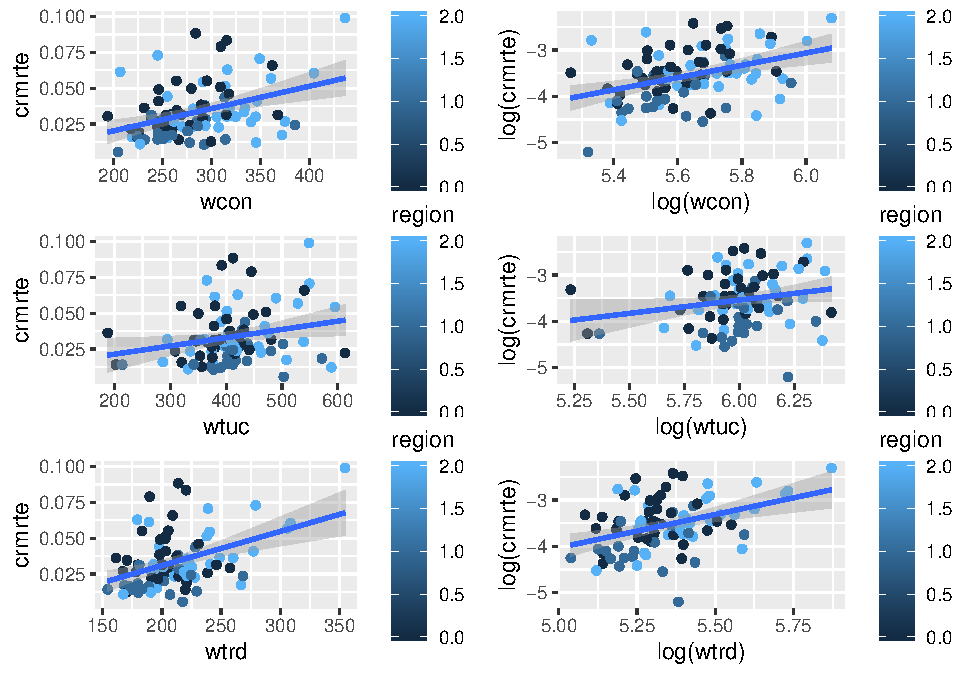
\includegraphics{Bagnard_Gaustad_Hartman_Leung_Lab_3_files/figure-latex/unnamed-chunk-50-1.pdf}

\begin{Shaded}
\begin{Highlighting}[]
\KeywordTok{grid.arrange}\NormalTok{(q4, q4a, q5, q5a, q6, q6a, }\DataTypeTok{ncol=}\DecValTok{2}\NormalTok{)}
\end{Highlighting}
\end{Shaded}

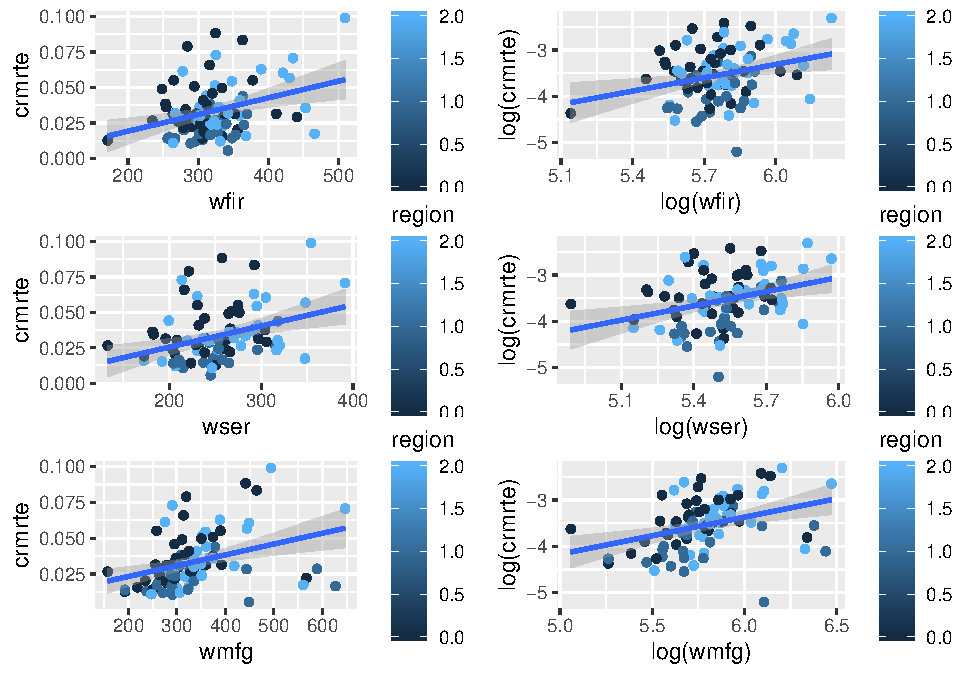
\includegraphics{Bagnard_Gaustad_Hartman_Leung_Lab_3_files/figure-latex/unnamed-chunk-50-2.pdf}

\begin{Shaded}
\begin{Highlighting}[]
\KeywordTok{grid.arrange}\NormalTok{(q7, q7a, q8, q8a, q9, q9a, }\DataTypeTok{ncol=}\DecValTok{2}\NormalTok{)}
\end{Highlighting}
\end{Shaded}

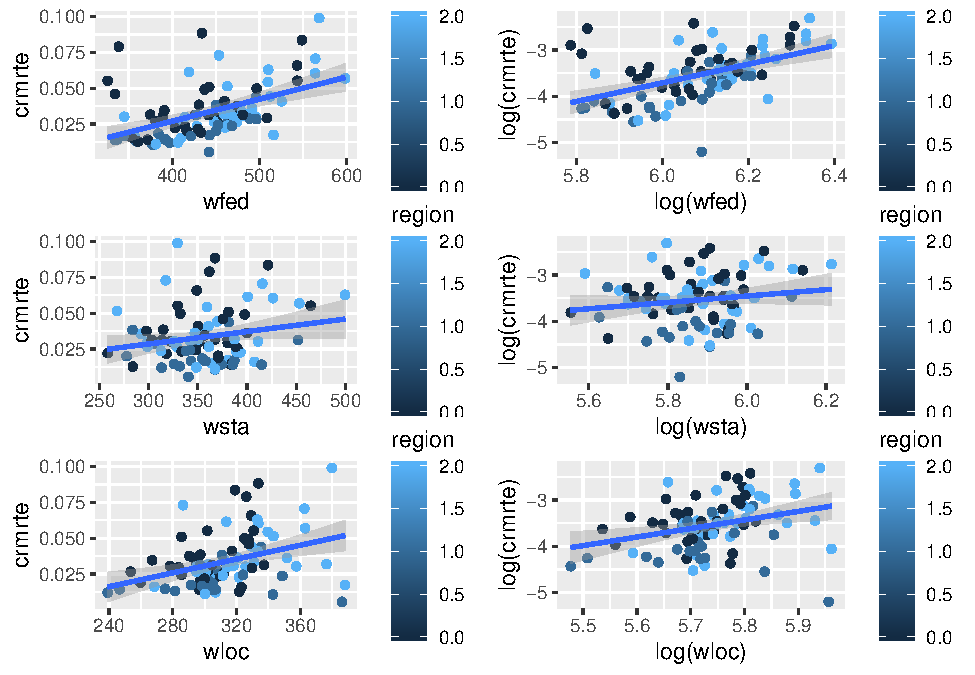
\includegraphics{Bagnard_Gaustad_Hartman_Leung_Lab_3_files/figure-latex/unnamed-chunk-50-3.pdf}

The transforms make the relationship more linearly distributed. We will
transform these variables to their log equivalents.

\begin{Shaded}
\begin{Highlighting}[]
\NormalTok{dfCrime}\OperatorTok{$}\NormalTok{logwcon<-}\KeywordTok{log}\NormalTok{(dfCrime}\OperatorTok{$}\NormalTok{wcon)}
\NormalTok{dfCrime}\OperatorTok{$}\NormalTok{logwtuc<-}\KeywordTok{log}\NormalTok{(dfCrime}\OperatorTok{$}\NormalTok{wtuc)}
\NormalTok{dfCrime}\OperatorTok{$}\NormalTok{logwtrd<-}\KeywordTok{log}\NormalTok{(dfCrime}\OperatorTok{$}\NormalTok{wtrd)}
\NormalTok{dfCrime}\OperatorTok{$}\NormalTok{logwfir<-}\KeywordTok{log}\NormalTok{(dfCrime}\OperatorTok{$}\NormalTok{wfir)}
\NormalTok{dfCrime}\OperatorTok{$}\NormalTok{logwser<-}\KeywordTok{log}\NormalTok{(dfCrime}\OperatorTok{$}\NormalTok{wser)}
\NormalTok{dfCrime}\OperatorTok{$}\NormalTok{logwmfg<-}\KeywordTok{log}\NormalTok{(dfCrime}\OperatorTok{$}\NormalTok{wmfg)}
\NormalTok{dfCrime}\OperatorTok{$}\NormalTok{logwfed<-}\KeywordTok{log}\NormalTok{(dfCrime}\OperatorTok{$}\NormalTok{wfed)}
\NormalTok{dfCrime}\OperatorTok{$}\NormalTok{logwsta<-}\KeywordTok{log}\NormalTok{(dfCrime}\OperatorTok{$}\NormalTok{wsta)}
\NormalTok{dfCrime}\OperatorTok{$}\NormalTok{logwloc<-}\KeywordTok{log}\NormalTok{(dfCrime}\OperatorTok{$}\NormalTok{wloc)}
\end{Highlighting}
\end{Shaded}

We move to the justice an law enforcement variables. With these
variables being mostly \textless{} 1 we'll also take the log for
comparison.

\begin{Shaded}
\begin{Highlighting}[]
\CommentTok{#Plot of the criminal justice and law enforcment related variables vs crmrte}
\NormalTok{q1<-}\KeywordTok{ggplot}\NormalTok{(}\DataTypeTok{data =}\NormalTok{ dfCrime, }\KeywordTok{aes}\NormalTok{(}\DataTypeTok{x =}\NormalTok{ prbarr, }\DataTypeTok{y =}\NormalTok{ crmrte, }\DataTypeTok{color =}\NormalTok{ region)) }\OperatorTok{+}\StringTok{ }
\StringTok{      }\KeywordTok{geom_point}\NormalTok{()}\OperatorTok{+}
\StringTok{  }\KeywordTok{geom_smooth}\NormalTok{(}\DataTypeTok{method =} \StringTok{"lm"}\NormalTok{)}
\NormalTok{q1a<-}\KeywordTok{ggplot}\NormalTok{(}\DataTypeTok{data =}\NormalTok{ dfCrime, }\KeywordTok{aes}\NormalTok{(}\DataTypeTok{x =} \KeywordTok{log}\NormalTok{(prbarr), }\DataTypeTok{y =} \KeywordTok{log}\NormalTok{(crmrte), }\DataTypeTok{color =}\NormalTok{ region)) }\OperatorTok{+}\StringTok{ }
\StringTok{      }\KeywordTok{geom_point}\NormalTok{()}\OperatorTok{+}
\StringTok{  }\KeywordTok{geom_smooth}\NormalTok{(}\DataTypeTok{method =} \StringTok{"lm"}\NormalTok{)}
\NormalTok{q2<-}\KeywordTok{ggplot}\NormalTok{(}\DataTypeTok{data =}\NormalTok{ dfCrime, }\KeywordTok{aes}\NormalTok{(}\DataTypeTok{x =}\NormalTok{ prbconv, }\DataTypeTok{y =}\NormalTok{ crmrte, }\DataTypeTok{color =}\NormalTok{ region)) }\OperatorTok{+}\StringTok{ }
\StringTok{      }\KeywordTok{geom_point}\NormalTok{()}\OperatorTok{+}
\StringTok{  }\KeywordTok{geom_smooth}\NormalTok{(}\DataTypeTok{method =} \StringTok{"lm"}\NormalTok{)}
\NormalTok{q2a<-}\KeywordTok{ggplot}\NormalTok{(}\DataTypeTok{data =}\NormalTok{ dfCrime, }\KeywordTok{aes}\NormalTok{(}\DataTypeTok{x =} \KeywordTok{log}\NormalTok{(prbconv), }\DataTypeTok{y =} \KeywordTok{log}\NormalTok{(crmrte), }\DataTypeTok{color =}\NormalTok{ region)) }\OperatorTok{+}\StringTok{ }
\StringTok{      }\KeywordTok{geom_point}\NormalTok{()}\OperatorTok{+}
\StringTok{  }\KeywordTok{geom_smooth}\NormalTok{(}\DataTypeTok{method =} \StringTok{"lm"}\NormalTok{)}
\NormalTok{q3<-}\KeywordTok{ggplot}\NormalTok{(}\DataTypeTok{data =}\NormalTok{ dfCrime, }\KeywordTok{aes}\NormalTok{(}\DataTypeTok{x =}\NormalTok{ prbpris, }\DataTypeTok{y =}\NormalTok{ crmrte, }\DataTypeTok{color =}\NormalTok{ region)) }\OperatorTok{+}\StringTok{ }
\StringTok{      }\KeywordTok{geom_point}\NormalTok{()}\OperatorTok{+}
\StringTok{  }\KeywordTok{geom_smooth}\NormalTok{(}\DataTypeTok{method =} \StringTok{"lm"}\NormalTok{)}
\NormalTok{q3a<-}\KeywordTok{ggplot}\NormalTok{(}\DataTypeTok{data =}\NormalTok{ dfCrime, }\KeywordTok{aes}\NormalTok{(}\DataTypeTok{x =} \KeywordTok{log}\NormalTok{(prbpris), }\DataTypeTok{y =} \KeywordTok{log}\NormalTok{(crmrte), }\DataTypeTok{color =}\NormalTok{ region)) }\OperatorTok{+}\StringTok{ }
\StringTok{      }\KeywordTok{geom_point}\NormalTok{()}\OperatorTok{+}
\StringTok{  }\KeywordTok{geom_smooth}\NormalTok{(}\DataTypeTok{method =} \StringTok{"lm"}\NormalTok{)}
\NormalTok{q4<-}\KeywordTok{ggplot}\NormalTok{(}\DataTypeTok{data =}\NormalTok{ dfCrime, }\KeywordTok{aes}\NormalTok{(}\DataTypeTok{x =}\NormalTok{ avgsen, }\DataTypeTok{y =}\NormalTok{ crmrte, }\DataTypeTok{color =}\NormalTok{ region)) }\OperatorTok{+}\StringTok{ }
\StringTok{      }\KeywordTok{geom_point}\NormalTok{()}\OperatorTok{+}
\StringTok{  }\KeywordTok{geom_smooth}\NormalTok{(}\DataTypeTok{method =} \StringTok{"lm"}\NormalTok{)}
\NormalTok{q4a<-}\KeywordTok{ggplot}\NormalTok{(}\DataTypeTok{data =}\NormalTok{ dfCrime, }\KeywordTok{aes}\NormalTok{(}\DataTypeTok{x =} \KeywordTok{log}\NormalTok{(avgsen), }\DataTypeTok{y =} \KeywordTok{log}\NormalTok{(crmrte), }\DataTypeTok{color =}\NormalTok{ region)) }\OperatorTok{+}\StringTok{ }
\StringTok{      }\KeywordTok{geom_point}\NormalTok{()}\OperatorTok{+}
\StringTok{  }\KeywordTok{geom_smooth}\NormalTok{(}\DataTypeTok{method =} \StringTok{"lm"}\NormalTok{)}
\NormalTok{q5<-}\KeywordTok{ggplot}\NormalTok{(}\DataTypeTok{data =}\NormalTok{ dfCrime, }\KeywordTok{aes}\NormalTok{(}\DataTypeTok{x =}\NormalTok{ polpc, }\DataTypeTok{y =}\NormalTok{ crmrte, }\DataTypeTok{color =}\NormalTok{ region)) }\OperatorTok{+}\StringTok{ }
\StringTok{      }\KeywordTok{geom_point}\NormalTok{()}\OperatorTok{+}
\StringTok{  }\KeywordTok{geom_smooth}\NormalTok{(}\DataTypeTok{method =} \StringTok{"lm"}\NormalTok{)}
\NormalTok{q5a<-}\KeywordTok{ggplot}\NormalTok{(}\DataTypeTok{data =}\NormalTok{ dfCrime, }\KeywordTok{aes}\NormalTok{(}\DataTypeTok{x =} \KeywordTok{log}\NormalTok{(polpc), }\DataTypeTok{y =} \KeywordTok{log}\NormalTok{(crmrte), }\DataTypeTok{color =}\NormalTok{ region)) }\OperatorTok{+}\StringTok{ }
\StringTok{      }\KeywordTok{geom_point}\NormalTok{()}\OperatorTok{+}
\StringTok{  }\KeywordTok{geom_smooth}\NormalTok{(}\DataTypeTok{method =} \StringTok{"lm"}\NormalTok{)}
\NormalTok{q6<-}\KeywordTok{ggplot}\NormalTok{(}\DataTypeTok{data =}\NormalTok{ dfCrime, }\KeywordTok{aes}\NormalTok{(}\DataTypeTok{x =}\NormalTok{ mix, }\DataTypeTok{y =}\NormalTok{ crmrte, }\DataTypeTok{color =}\NormalTok{ region)) }\OperatorTok{+}\StringTok{ }
\StringTok{      }\KeywordTok{geom_point}\NormalTok{()}\OperatorTok{+}
\StringTok{  }\KeywordTok{geom_smooth}\NormalTok{(}\DataTypeTok{method =} \StringTok{"lm"}\NormalTok{)}
\NormalTok{q6a<-}\KeywordTok{ggplot}\NormalTok{(}\DataTypeTok{data =}\NormalTok{ dfCrime, }\KeywordTok{aes}\NormalTok{(}\DataTypeTok{x =} \KeywordTok{log}\NormalTok{(mix), }\DataTypeTok{y =} \KeywordTok{log}\NormalTok{(crmrte), }\DataTypeTok{color =}\NormalTok{ region)) }\OperatorTok{+}\StringTok{ }
\StringTok{      }\KeywordTok{geom_point}\NormalTok{()}\OperatorTok{+}
\StringTok{  }\KeywordTok{geom_smooth}\NormalTok{(}\DataTypeTok{method =} \StringTok{"lm"}\NormalTok{)}

\KeywordTok{grid.arrange}\NormalTok{(q1, q1a, q2, q2a, q3, q3a, }\DataTypeTok{ncol=}\DecValTok{2}\NormalTok{)}
\end{Highlighting}
\end{Shaded}

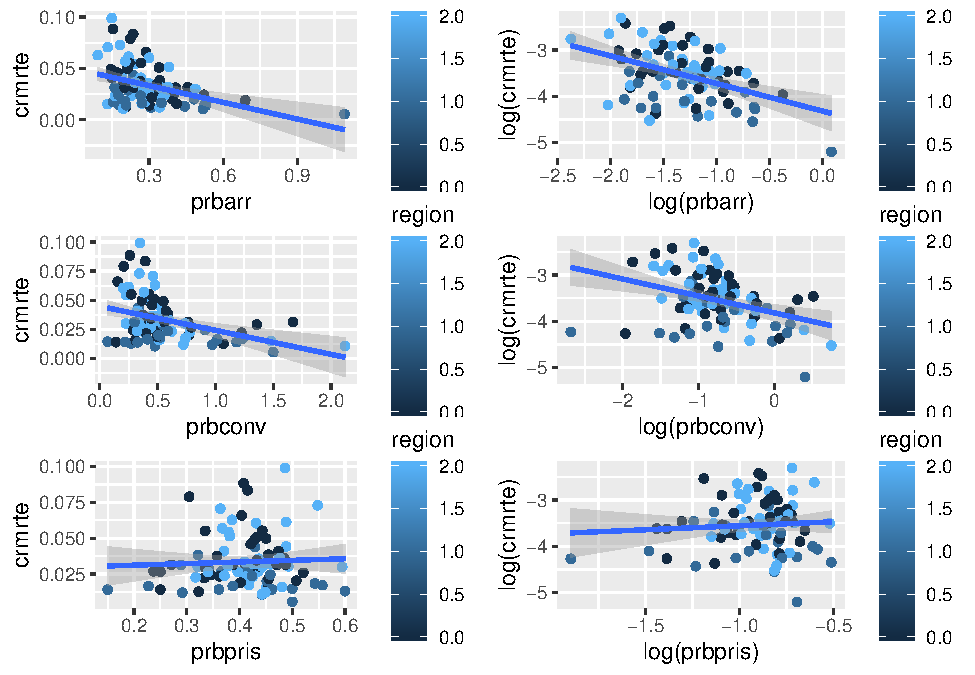
\includegraphics{Bagnard_Gaustad_Hartman_Leung_Lab_3_files/figure-latex/unnamed-chunk-52-1.pdf}

\begin{Shaded}
\begin{Highlighting}[]
\KeywordTok{grid.arrange}\NormalTok{(q4, q4a, q5, q5a, q6, q6a, }\DataTypeTok{ncol=}\DecValTok{2}\NormalTok{)}
\end{Highlighting}
\end{Shaded}

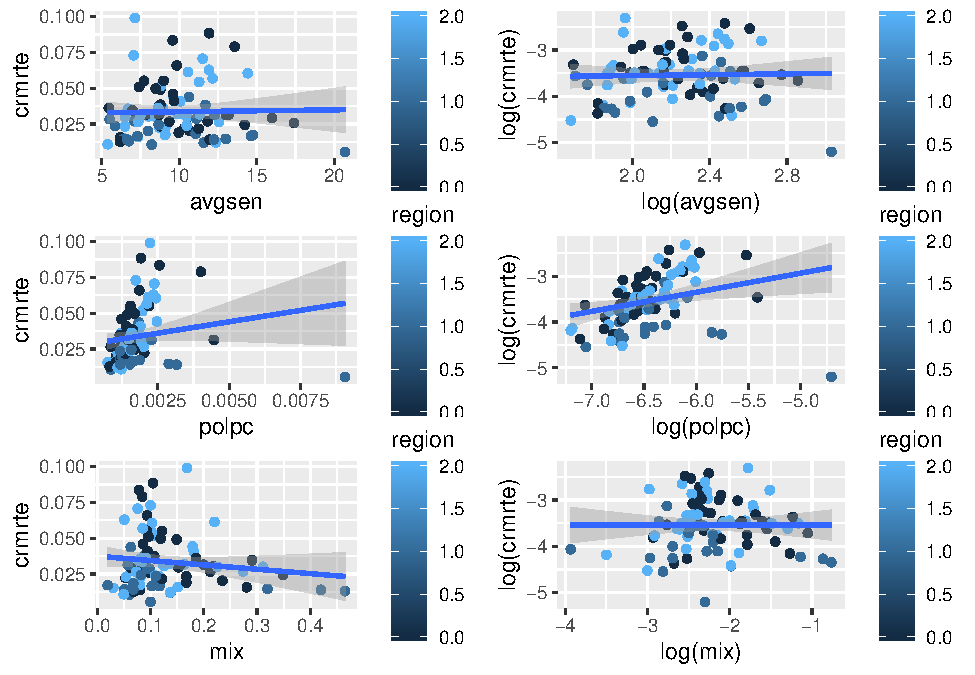
\includegraphics{Bagnard_Gaustad_Hartman_Leung_Lab_3_files/figure-latex/unnamed-chunk-52-2.pdf}

The log transformation for these variables makes the relationship more
linear. We will transform these variables to their log equivalents.

We also note that of the six variables, only prbarr, prbconv and polpc
show univariate correlation with crime. We believe these will be better
candidates for our model selection. Further, we see mix has no
correlation with crmrate and may be its own outcome variable.

\begin{Shaded}
\begin{Highlighting}[]
\NormalTok{dfCrime}\OperatorTok{$}\NormalTok{logprbarr <-}\StringTok{ }\KeywordTok{log}\NormalTok{(dfCrime}\OperatorTok{$}\NormalTok{prbarr)}
\NormalTok{dfCrime}\OperatorTok{$}\NormalTok{logprbconv <-}\StringTok{ }\KeywordTok{log}\NormalTok{(dfCrime}\OperatorTok{$}\NormalTok{prbconv)}
\NormalTok{dfCrime}\OperatorTok{$}\NormalTok{logprbpris <-}\StringTok{ }\KeywordTok{log}\NormalTok{(dfCrime}\OperatorTok{$}\NormalTok{prbpris)}
\NormalTok{dfCrime}\OperatorTok{$}\NormalTok{logavgsen <-}\StringTok{ }\KeywordTok{log}\NormalTok{(dfCrime}\OperatorTok{$}\NormalTok{avgsen)}
\NormalTok{dfCrime}\OperatorTok{$}\NormalTok{logpolpc <-}\StringTok{ }\KeywordTok{log}\NormalTok{(dfCrime}\OperatorTok{$}\NormalTok{polpc)}
\NormalTok{dfCrime}\OperatorTok{$}\NormalTok{logmix <-}\StringTok{ }\KeywordTok{log}\NormalTok{(dfCrime}\OperatorTok{$}\NormalTok{mix)}
\end{Highlighting}
\end{Shaded}

Next we take a look at the demographic variables and their log
alternatives

\begin{Shaded}
\begin{Highlighting}[]
\NormalTok{q1<-}\KeywordTok{ggplot}\NormalTok{(}\DataTypeTok{data =}\NormalTok{ dfCrime, }\KeywordTok{aes}\NormalTok{(}\DataTypeTok{x =}\NormalTok{ pctymle, }\DataTypeTok{y =}\NormalTok{ crmrte, }\DataTypeTok{color =}\NormalTok{ region)) }\OperatorTok{+}\StringTok{ }
\StringTok{      }\KeywordTok{geom_point}\NormalTok{()}\OperatorTok{+}
\StringTok{  }\KeywordTok{geom_smooth}\NormalTok{(}\DataTypeTok{method =} \StringTok{"lm"}\NormalTok{)}
\NormalTok{q1a<-}\KeywordTok{ggplot}\NormalTok{(}\DataTypeTok{data =}\NormalTok{ dfCrime, }\KeywordTok{aes}\NormalTok{(}\DataTypeTok{x =} \KeywordTok{log}\NormalTok{(pctymle), }\DataTypeTok{y =} \KeywordTok{log}\NormalTok{(crmrte), }\DataTypeTok{color =}\NormalTok{ region)) }\OperatorTok{+}\StringTok{ }
\StringTok{      }\KeywordTok{geom_point}\NormalTok{()}\OperatorTok{+}
\StringTok{  }\KeywordTok{geom_smooth}\NormalTok{(}\DataTypeTok{method =} \StringTok{"lm"}\NormalTok{)}
\NormalTok{q2<-}\KeywordTok{ggplot}\NormalTok{(}\DataTypeTok{data =}\NormalTok{ dfCrime, }\KeywordTok{aes}\NormalTok{(}\DataTypeTok{x =}\NormalTok{ pctmin80, }\DataTypeTok{y =}\NormalTok{ crmrte, }\DataTypeTok{color =}\NormalTok{ region)) }\OperatorTok{+}\StringTok{ }
\StringTok{      }\KeywordTok{geom_point}\NormalTok{()}\OperatorTok{+}
\StringTok{  }\KeywordTok{geom_smooth}\NormalTok{(}\DataTypeTok{method =} \StringTok{"lm"}\NormalTok{)}
\NormalTok{q2a<-}\KeywordTok{ggplot}\NormalTok{(}\DataTypeTok{data =}\NormalTok{ dfCrime, }\KeywordTok{aes}\NormalTok{(}\DataTypeTok{x =} \KeywordTok{log}\NormalTok{(pctmin80), }\DataTypeTok{y =} \KeywordTok{log}\NormalTok{(crmrte), }\DataTypeTok{color =}\NormalTok{ region)) }\OperatorTok{+}\StringTok{ }
\StringTok{      }\KeywordTok{geom_point}\NormalTok{()}\OperatorTok{+}
\StringTok{  }\KeywordTok{geom_smooth}\NormalTok{(}\DataTypeTok{method =} \StringTok{"lm"}\NormalTok{)}
\NormalTok{q3<-}\KeywordTok{ggplot}\NormalTok{(}\DataTypeTok{data =}\NormalTok{ dfCrime, }\KeywordTok{aes}\NormalTok{(}\DataTypeTok{x =}\NormalTok{ density, }\DataTypeTok{y =}\NormalTok{ crmrte, }\DataTypeTok{color =}\NormalTok{ region)) }\OperatorTok{+}\StringTok{ }
\StringTok{      }\KeywordTok{geom_point}\NormalTok{()}\OperatorTok{+}
\StringTok{  }\KeywordTok{geom_smooth}\NormalTok{(}\DataTypeTok{method =} \StringTok{"lm"}\NormalTok{)}
\NormalTok{q3a<-}\KeywordTok{ggplot}\NormalTok{(}\DataTypeTok{data =}\NormalTok{ dfCrime, }\KeywordTok{aes}\NormalTok{(}\DataTypeTok{x =} \KeywordTok{log}\NormalTok{(density), }\DataTypeTok{y =} \KeywordTok{log}\NormalTok{(crmrte), }\DataTypeTok{color =}\NormalTok{ region)) }\OperatorTok{+}\StringTok{ }
\StringTok{      }\KeywordTok{geom_point}\NormalTok{()}\OperatorTok{+}
\StringTok{  }\KeywordTok{geom_smooth}\NormalTok{(}\DataTypeTok{method =} \StringTok{"lm"}\NormalTok{)}


\KeywordTok{grid.arrange}\NormalTok{(q1, q1a, q2, q2a, q3, q3a, }\DataTypeTok{ncol=}\DecValTok{2}\NormalTok{)}
\end{Highlighting}
\end{Shaded}

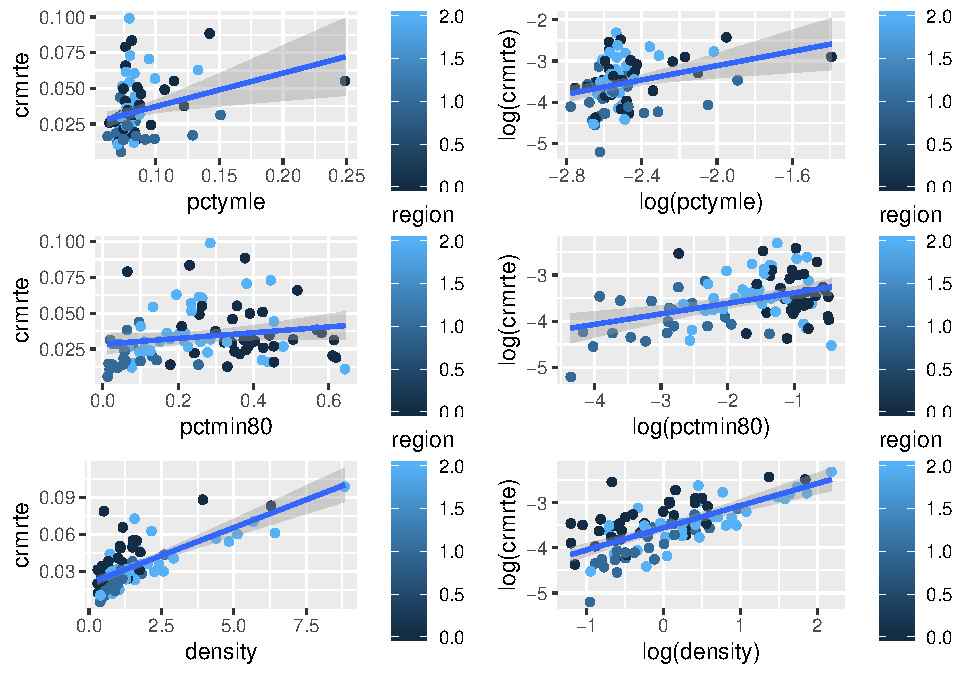
\includegraphics{Bagnard_Gaustad_Hartman_Leung_Lab_3_files/figure-latex/unnamed-chunk-54-1.pdf}

Again we see improvements after transformation. We will include
transforms of these variables as well.

\begin{Shaded}
\begin{Highlighting}[]
\NormalTok{dfCrime}\OperatorTok{$}\NormalTok{logdensity <-}\StringTok{ }\KeywordTok{log}\NormalTok{(dfCrime}\OperatorTok{$}\NormalTok{density)}
\NormalTok{dfCrime}\OperatorTok{$}\NormalTok{logpctmin80 <-}\StringTok{ }\KeywordTok{log}\NormalTok{(dfCrime}\OperatorTok{$}\NormalTok{pctmin80)}
\NormalTok{dfCrime}\OperatorTok{$}\NormalTok{logpctymle <-}\StringTok{ }\KeywordTok{log}\NormalTok{(dfCrime}\OperatorTok{$}\NormalTok{pctymle)}
\end{Highlighting}
\end{Shaded}

Finally, we'll take a look at taxpc and a histogram of the crmrte
variable itself.

\begin{Shaded}
\begin{Highlighting}[]
\NormalTok{q1<-}\KeywordTok{ggplot}\NormalTok{(}\DataTypeTok{data =}\NormalTok{ dfCrime, }\KeywordTok{aes}\NormalTok{(}\DataTypeTok{x =}\NormalTok{ taxpc, }\DataTypeTok{y =}\NormalTok{ crmrte, }\DataTypeTok{color =}\NormalTok{ region)) }\OperatorTok{+}\StringTok{ }
\StringTok{      }\KeywordTok{geom_point}\NormalTok{()}\OperatorTok{+}
\StringTok{  }\KeywordTok{geom_smooth}\NormalTok{(}\DataTypeTok{method =} \StringTok{"lm"}\NormalTok{)}
\NormalTok{q1a<-}\KeywordTok{ggplot}\NormalTok{(}\DataTypeTok{data =}\NormalTok{ dfCrime, }\KeywordTok{aes}\NormalTok{(}\DataTypeTok{x =} \KeywordTok{log}\NormalTok{(taxpc), }\DataTypeTok{y =} \KeywordTok{log}\NormalTok{(crmrte), }\DataTypeTok{color =}\NormalTok{ region)) }\OperatorTok{+}\StringTok{ }
\StringTok{      }\KeywordTok{geom_point}\NormalTok{()}\OperatorTok{+}
\StringTok{  }\KeywordTok{geom_smooth}\NormalTok{(}\DataTypeTok{method =} \StringTok{"lm"}\NormalTok{)}

\NormalTok{q2<-}\KeywordTok{ggplot}\NormalTok{(}\DataTypeTok{data =}\NormalTok{ dfCrime, }\KeywordTok{aes}\NormalTok{(}\DataTypeTok{x =}\NormalTok{ crmrte)) }\OperatorTok{+}\StringTok{ }
\StringTok{      }\KeywordTok{geom_histogram}\NormalTok{(}\DataTypeTok{bins=}\DecValTok{30}\NormalTok{)}
\NormalTok{q2a<-}\KeywordTok{ggplot}\NormalTok{(}\DataTypeTok{data =}\NormalTok{ dfCrime, }\KeywordTok{aes}\NormalTok{(}\DataTypeTok{x =} \KeywordTok{log}\NormalTok{(crmrte))) }\OperatorTok{+}\StringTok{ }
\StringTok{      }\KeywordTok{geom_histogram}\NormalTok{(}\DataTypeTok{bins=}\DecValTok{30}\NormalTok{)}

\KeywordTok{grid.arrange}\NormalTok{(q1, q1a, q2, q2a, }\DataTypeTok{ncol=}\DecValTok{2}\NormalTok{)}
\end{Highlighting}
\end{Shaded}

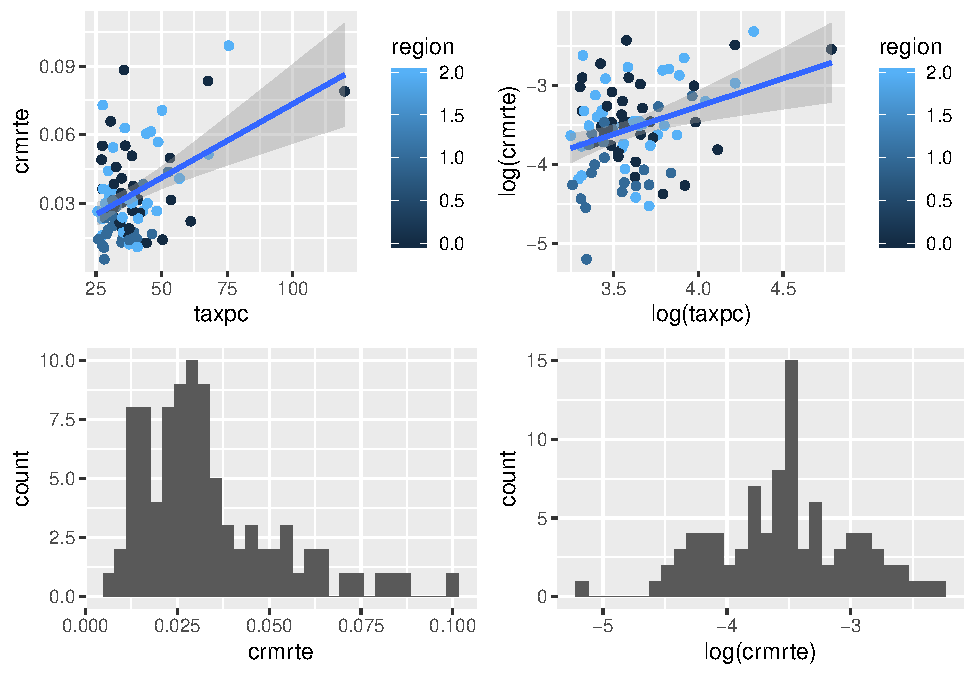
\includegraphics{Bagnard_Gaustad_Hartman_Leung_Lab_3_files/figure-latex/unnamed-chunk-56-1.pdf}

The crmrte and taxpc variables also show improvement after
transformation. We'll add those to our dataframe.

\begin{Shaded}
\begin{Highlighting}[]
\NormalTok{dfCrime}\OperatorTok{$}\NormalTok{logcrmrte =}\StringTok{ }\KeywordTok{log}\NormalTok{(dfCrime}\OperatorTok{$}\NormalTok{crmrte)}
\NormalTok{dfCrime}\OperatorTok{$}\NormalTok{logtaxpc =}\StringTok{ }\KeywordTok{log}\NormalTok{(dfCrime}\OperatorTok{$}\NormalTok{taxpc)}
\end{Highlighting}
\end{Shaded}

With our variables transformed, we now turn to discussion on
collinearity and multicollinearity in our data set. To facilitate the
discussion we'll draw reference to a network plot.

\begin{Shaded}
\begin{Highlighting}[]
\KeywordTok{options}\NormalTok{(}\DataTypeTok{repr.plot.width=}\DecValTok{8}\NormalTok{, }\DataTypeTok{repr.plot.height=}\DecValTok{8}\NormalTok{)}
\NormalTok{myData<-dfCrime}
\NormalTok{myData<-myData[, }\KeywordTok{c}\NormalTok{(}\StringTok{"logcrmrte"}\NormalTok{, }\StringTok{"west"}\NormalTok{, }\StringTok{"central"}\NormalTok{, }\StringTok{"other"}\NormalTok{, }\StringTok{"urban"}\NormalTok{, }\StringTok{"logprbarr"}\NormalTok{, }\StringTok{"logprbconv"}\NormalTok{, }\StringTok{"logprbpris"}\NormalTok{, }\StringTok{"logavgsen"}\NormalTok{, }\StringTok{"logpolpc"}\NormalTok{, }\StringTok{"logtaxpc"}\NormalTok{,}
           \StringTok{"logpctmin80"}\NormalTok{, }\StringTok{"logwcon"}\NormalTok{, }\StringTok{"logwtuc"}\NormalTok{, }\StringTok{"logwtrd"}\NormalTok{, }\StringTok{"logwfir"}\NormalTok{, }\StringTok{"logwser"}\NormalTok{, }\StringTok{"logwmfg"}\NormalTok{, }\StringTok{"logwfed"}\NormalTok{, }\StringTok{"logwsta"}\NormalTok{, }\StringTok{"logwloc"}\NormalTok{,}
           \StringTok{"logmix"}\NormalTok{, }\StringTok{"logpctymle"}\NormalTok{)]}
\NormalTok{plot<-myData }\OperatorTok\StringTok{ }\KeywordTok{correlate}\NormalTok{() }\OperatorTok\StringTok{ }\KeywordTok{network_plot}\NormalTok{(}\DataTypeTok{min_cor=}\NormalTok{.}\DecValTok{25}\NormalTok{)}
\end{Highlighting}
\end{Shaded}

\begin{verbatim}

Correlation method: 'pearson'
Missing treated using: 'pairwise.complete.obs'
\end{verbatim}

\begin{Shaded}
\begin{Highlighting}[]
\KeywordTok{grid.arrange}\NormalTok{(}\KeywordTok{arrangeGrob}\NormalTok{(plot, }\DataTypeTok{bottom =} \StringTok{'Correlation Plot'}\NormalTok{), }
             \DataTypeTok{top =} \StringTok{"Correlation plots for Independent Variables"}\NormalTok{, }\DataTypeTok{ncol=}\DecValTok{1}\NormalTok{)}
\end{Highlighting}
\end{Shaded}

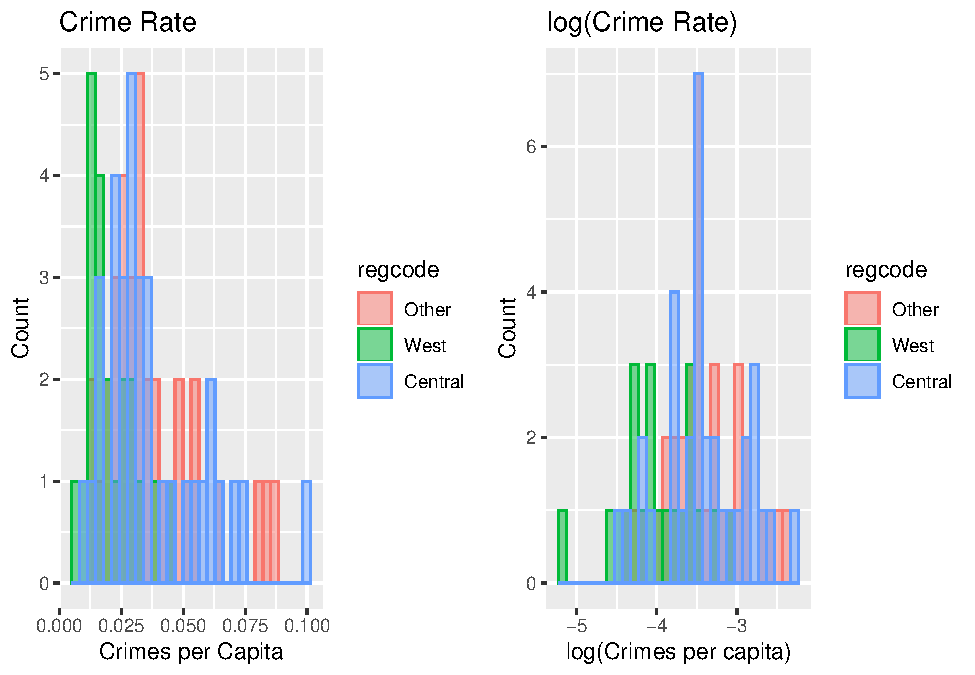
\includegraphics{Bagnard_Gaustad_Hartman_Leung_Lab_3_files/figure-latex/unnamed-chunk-58-1.pdf}
First, we note the general proximity of variables with one another.
Variables that are clustered together have stronger affinities and
degrees of collinearity. In fact, the cluster of the wage variables are
an indication of multicollinearity. Only state wages fall outside this
group. The telecome and utlity wage variable, while still near the
cluster, show a little less collinearity. If we choose to operationalize
the wage variables we must pick an appropriate strategy to minimize
their multicollinearity impact. We also see the wage variables are
positively correlated with our crime outcome variable.

Next, we notice the Law enforcement and Judicial variables are clustered
and have a negative correlation with our outcome variable on crime. We
also see they tend to be negatively correlated amongst one another. For
example, probability of conviction is slightly negatively corrrelated
with the probability of arrest, and both are negatively correlated with
our outcome variable. We may wish to combine their impacts. We also see
that police per capita and tax per capita are positively correlated with
another. This makes sense as the more revenues collected the higher the
ability to pay for community services such as law enforcement and
protection. Both are also positively correlated with our outcome
variable on crime. We also notice that percent young male has a positive
correlation with crime rate. A possible explanation for this is that
more crimes are committed by younger men as a whole. We also note that
counties with higher state wages are correlated with higher percentages
of young males, and these two variables are clustered together.

The mix variable is an odd one. It is positively correlated with
probability of arrests, negatively correlated with probability of
convictions, and negatively correlated with service wages and
manufacturing wages. It also has a slight positive correlation with the
state wage and seems to be clustered with it.

Last, we turn to our region variables and notice the high negative
correlation of the minority variable with the western region. We also
notice a high positive corrlation of minorities with the `other'
(eastern) region. This variable also correlates positively with crime
rate, although the two are not clustered. We especially note that west
is negatively correlated with crime rate. There appears to be a lessor
propensity for crime in this region. We will examine this phenomenom
further. Also, for a futher examination of correlation plots for each of
the regions please see the network diagrams in the appendix.

\hypertarget{additional-variables-to-operationalize}{%
\subsection{Additional Variables to
Operationalize}\label{additional-variables-to-operationalize}}

As a final point of discussion we will identify variables we wish to
operationalize for use in our models. We will include a variable that
expresses the economic condition of the county and a variable that
expresses criminal justice effectiveness.

The first variable on the economic condition will include the sum of all
average weekly wages from the 1980 census information. Since we do not
know how many were employed at that wage we use this summary the best
available proxy. Summing the wages into one variable will also remove
their multicollinearity effects.

\begin{Shaded}
\begin{Highlighting}[]
\NormalTok{dfCrime}\OperatorTok{$}\NormalTok{allWages<-dfCrime}\OperatorTok{$}\NormalTok{wcon }\OperatorTok{+}\StringTok{ }\NormalTok{dfCrime}\OperatorTok{$}\NormalTok{wtuc }\OperatorTok{+}\StringTok{ }\NormalTok{dfCrime}\OperatorTok{$}\NormalTok{wtrd }\OperatorTok{+}\StringTok{ }\NormalTok{dfCrime}\OperatorTok{$}\NormalTok{wfir }\OperatorTok{+}
\StringTok{    }\NormalTok{dfCrime}\OperatorTok{$}\NormalTok{wser }\OperatorTok{+}\StringTok{ }\NormalTok{dfCrime}\OperatorTok{$}\NormalTok{wmfg }\OperatorTok{+}\StringTok{ }\NormalTok{dfCrime}\OperatorTok{$}\NormalTok{wfed }\OperatorTok{+}\StringTok{ }\NormalTok{dfCrime}\OperatorTok{$}\NormalTok{wsta }\OperatorTok{+}\StringTok{ }\NormalTok{dfCrime}\OperatorTok{$}\NormalTok{wloc}
\end{Highlighting}
\end{Shaded}

As a second variable, we are interested in understanding the
effectiveness of the criminal justice system as a crime deterrent. Our
proxy will be the number of convictions per incident.

This is operationalized by taking the probability of arrests, pbrarr
(which is defined as arrests per incident) and multiplying by the
probability of convictions, pbrconv (which is defined as convictions per
arrest). The new variable is defined below.

\begin{Shaded}
\begin{Highlighting}[]
\NormalTok{dfCrime}\OperatorTok{$}\NormalTok{crimJustEff<-dfCrime}\OperatorTok{$}\NormalTok{prbarr }\OperatorTok{*}\StringTok{ }\NormalTok{dfCrime}\OperatorTok{$}\NormalTok{prbconv}
\end{Highlighting}
\end{Shaded}

We will also create a logarithmic transformation of this variable based
on our histogram analysis from before.

\begin{Shaded}
\begin{Highlighting}[]
\NormalTok{dfCrime}\OperatorTok{$}\NormalTok{logcrimJustEff<-}\KeywordTok{log}\NormalTok{(dfCrime}\OperatorTok{$}\NormalTok{crimJustEff)}
\end{Highlighting}
\end{Shaded}

\hypertarget{summary-and-results}{%
\subsection{Summary and Results}\label{summary-and-results}}

Our outcome variable is the \emph{crime rate} (``crmrte''), which is
defined as the crimes committed per person in a specific county during
1987. The crime rate of the 90 counties in our sample dataset range
between 0.0055 - 0.0990, with a mean of 0.0335.

From the boxplot below, most of the counties have a crime rate between
0.0055 and 0.0700, with 5 outliers having a crime rate \textgreater{}
0.0700.

\begin{Shaded}
\begin{Highlighting}[]
\KeywordTok{options}\NormalTok{(}\DataTypeTok{repr.plot.width=}\DecValTok{3}\NormalTok{, }\DataTypeTok{repr.plot.height=}\DecValTok{4}\NormalTok{)}
\KeywordTok{ggplot}\NormalTok{(}\DataTypeTok{data =}\NormalTok{ dfCrime, }\KeywordTok{aes}\NormalTok{(}\DataTypeTok{y =}\NormalTok{ crmrte)) }\OperatorTok{+}\StringTok{ }
\StringTok{      }\KeywordTok{geom_boxplot}\NormalTok{()}
\end{Highlighting}
\end{Shaded}

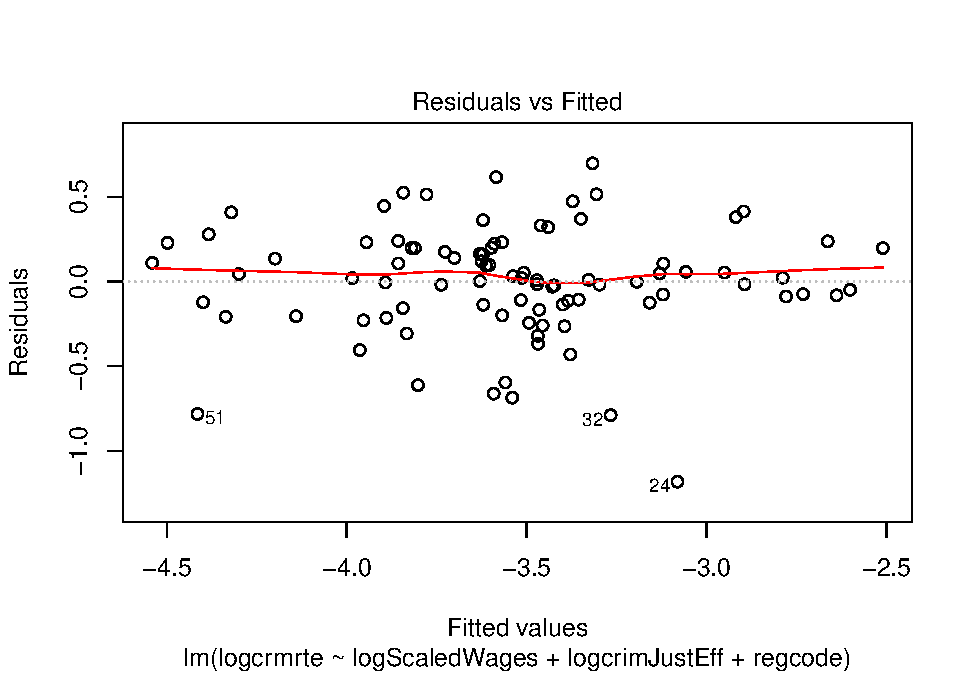
\includegraphics{Bagnard_Gaustad_Hartman_Leung_Lab_3_files/figure-latex/unnamed-chunk-62-1.pdf}

While mix (the type of crime committed) is also potentially an outcome
variable, our research focuses on providing policy recommendations to
reduce crime in general and not a specific type of crime. Mix is also
not a linear outcome and hence difficult to measure.

We propose 3 multiple linear regression models

\begin{itemize}
\item
  First Model: Has only the explanatory variables of key interest and no
  other covariates.
\item
  Second Model: Includes the explanatory variables and covariates that
  increase the accuracy of our results without substantial bias.
\item
  Third Model: An expansion of the second model with most covariates,
  designed to demonstrate the robustness of our results to model
  specification.
\end{itemize}

As we proceed with each model, we verify the CLM assumptions of OLS are
addressed below:

\begin{itemize}
\tightlist
\item
  \textbf{MLR1} Linear in parameters: The models have had its data
  transformed as described above to allow a linear fit of the model.
\item
  \textbf{MLR2} Random Sampling: The data is collected from a data set
  with rolled up data for each county. It is not randomly sampled by
  area or population.
\item
  \textbf{MLR3} No perfect multicollinearity: None of the variables
  chosen for the model are constant or perfectly collinear as
  demonstrated by the scatterplot below.
\item
  \textbf{MLR4'} The expectation of u and and covariance of each
  regressor with u are \textasciitilde{}0. This shows that our model's
  regressors are exogenous with the error.
\item
  \textbf{MLR5'} Spherical errors: There is homoscedasticity and no
  autocorrelation {[}TBD{]}.
\item
  \textbf{MLR6'} Our error terms should be normally distributed
  {[}TBD{]}.
\end{itemize}

By satisfying these assumptions, we can expect our coefficients will be
approaching the true parameter values in probability.

\hypertarget{evidence-of-multi-collinearity-or-perfect-collinearity}{%
\paragraph{Evidence of multi-collinearity (or perfect
collinearity)?}\label{evidence-of-multi-collinearity-or-perfect-collinearity}}

\begin{Shaded}
\begin{Highlighting}[]
\KeywordTok{options}\NormalTok{(}\DataTypeTok{repr.plot.width=}\DecValTok{8}\NormalTok{, }\DataTypeTok{repr.plot.height=}\DecValTok{8}\NormalTok{)}
\KeywordTok{pairs}\NormalTok{(}\OperatorTok{~}\StringTok{ }\NormalTok{logcrimJustEff }\OperatorTok{+}\StringTok{ }\NormalTok{logpolpc }\OperatorTok{+}\StringTok{ }\NormalTok{allWages }\OperatorTok{+}\StringTok{ }\NormalTok{logtaxpc }\OperatorTok{+}\StringTok{ }\NormalTok{logdensity }\OperatorTok{+}\StringTok{ }\NormalTok{logpctmin80 }\OperatorTok{+}
\StringTok{        }\NormalTok{logpctymle, }\DataTypeTok{data=}\NormalTok{dfCrime, }\DataTypeTok{main=}\StringTok{"Scatterplot Matrix of Model Variables"}\NormalTok{)}
\end{Highlighting}
\end{Shaded}

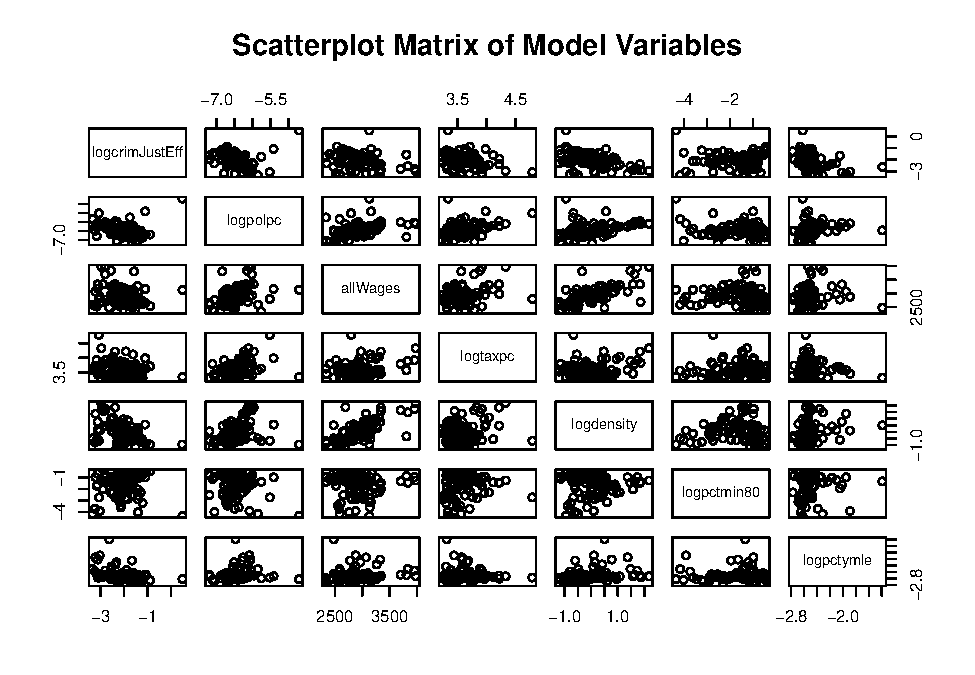
\includegraphics{Bagnard_Gaustad_Hartman_Leung_Lab_3_files/figure-latex/unnamed-chunk-63-1.pdf}

\hypertarget{model-analysis}{%
\section{Model Analysis}\label{model-analysis}}

\hypertarget{model-1}{%
\subsection{Model 1}\label{model-1}}

\hypertarget{introduction-1}{%
\subsubsection{Introduction}\label{introduction-1}}

Our base hypothesis is that crime can be fundamentally explained by two
factors: the effectiveness of the criminal justice system and the
economic conditions.

Criminal Justice Effectiveness is self defined : To be able to track
crimes, they must be reported to police, who can then make arrests and
the legal system provides judgement (convictions/sentencing) Criminal
justice also has a relationship to crime as a deterrent, as the
probability of getting caught, convicted, sentenced could potentially
deter crime.

We operationalize criminal justice effectiveness as (probability of
Convictions * Crimes committed). We define this as: prbconv * prbarr =
conv/arrest * arrest/crime = convictions/crime. Without more granular
data, this provides a single parsimonious metric that helps understand
how the law enforcement and criminal justice system works.

\hypertarget{model-1-eda}{%
\subsubsection{Model 1 EDA}\label{model-1-eda}}

\textbf{Data Transformations}

\begin{Shaded}
\begin{Highlighting}[]
\KeywordTok{options}\NormalTok{(}\DataTypeTok{repr.plot.width=}\DecValTok{4}\NormalTok{, }\DataTypeTok{repr.plot.height=}\DecValTok{4}\NormalTok{)}
\KeywordTok{hist}\NormalTok{((dfCrime}\OperatorTok{$}\NormalTok{prbconv))}
\end{Highlighting}
\end{Shaded}

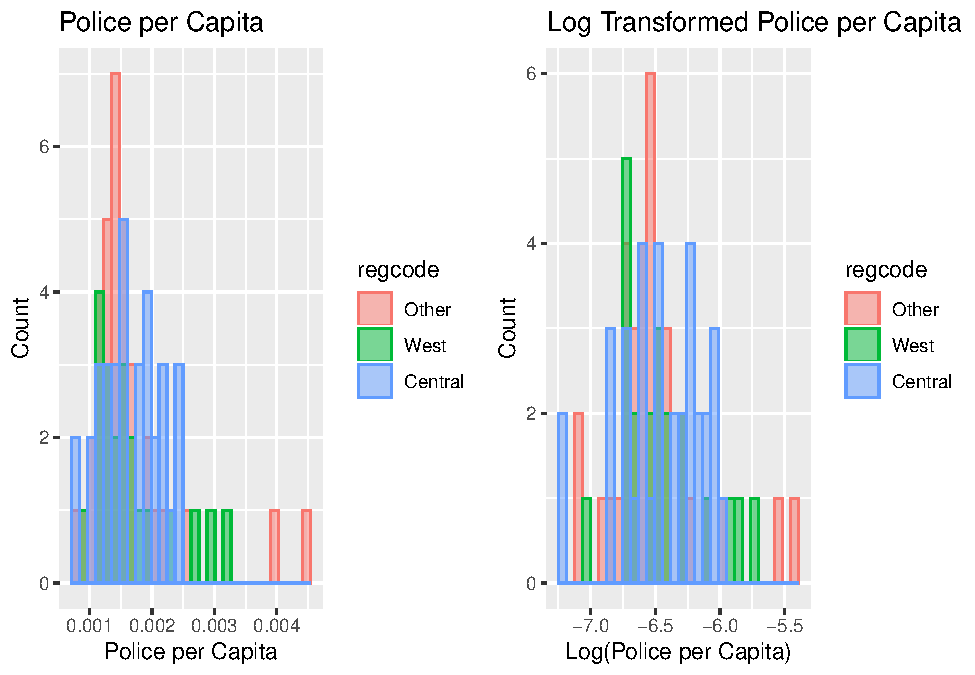
\includegraphics{Bagnard_Gaustad_Hartman_Leung_Lab_3_files/figure-latex/unnamed-chunk-64-1.pdf}

\begin{Shaded}
\begin{Highlighting}[]
\KeywordTok{hist}\NormalTok{((dfCrime}\OperatorTok{$}\NormalTok{prbarr))}
\end{Highlighting}
\end{Shaded}

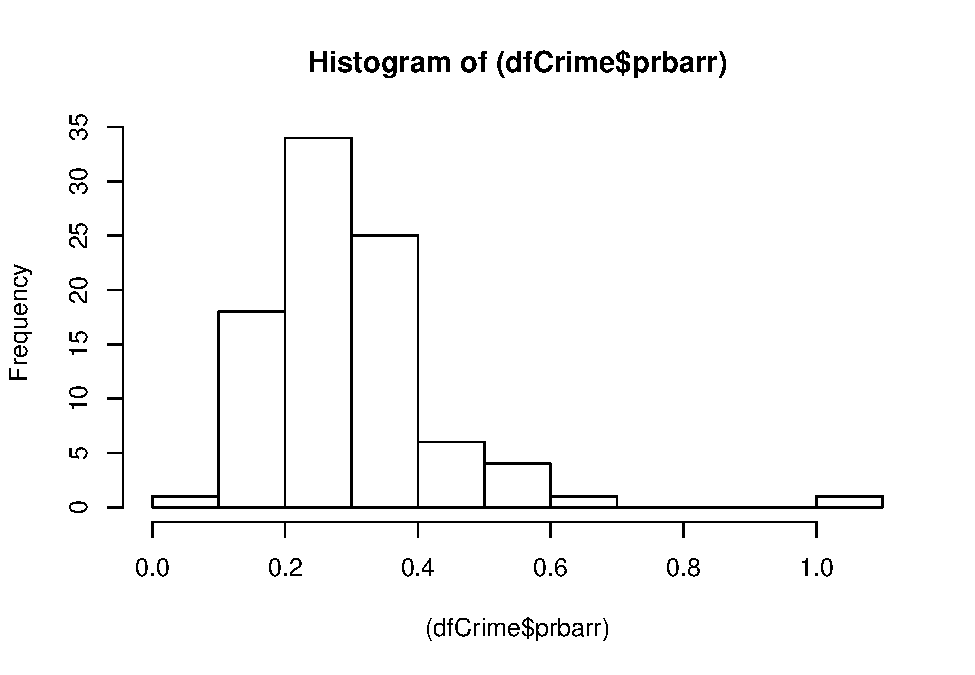
\includegraphics{Bagnard_Gaustad_Hartman_Leung_Lab_3_files/figure-latex/unnamed-chunk-64-2.pdf}

The distribution of both probability of conviction and probability of
arrest are peculiar and non-normal. It could be argued that both of
these variables should be bound between 0 and 1. However,
``probability'' of conviction is proxied by a ratio of convictions to
arrests. It is in fact common that defendents are charged with multiple
crimes and convicted, but were only arrested once.

For ``probability'' of arrest, it could be possible there are multiple
arrests for a single offense. However, the single data point that is
greater than one, is \textgreater{}3 standard deviations away from the
distribution. This outlier will have high leverage on our model and will
be preemptively removed as the data supplied is likely in error and is
not representative of the bulk of North Carolina counties.

For parsimony, we can simply the probability of arrest and probability
of conviction by multiplying to effectively get the ratio of convictions
to offenses. The normality of this factor can be improved by taking a
log transform. QQ plots help to visualize how normality improves for the
inner quartiles.

\begin{Shaded}
\begin{Highlighting}[]
\CommentTok{# how many standard deviations away the outlier lies}
\NormalTok{(dfCrime[}\DecValTok{51}\NormalTok{,]}\OperatorTok{$}\NormalTok{prbarr }\OperatorTok{-}\StringTok{ }\KeywordTok{mean}\NormalTok{(dfCrime}\OperatorTok{$}\NormalTok{prbarr))}\OperatorTok{/}\KeywordTok{sd}\NormalTok{(dfCrime}\OperatorTok{$}\NormalTok{prbarr) }
\end{Highlighting}
\end{Shaded}

\begin{verbatim}
[1] 5.779438
\end{verbatim}

\begin{Shaded}
\begin{Highlighting}[]
\CommentTok{#hist(log(dfCrime$crimJustEff))}
\KeywordTok{ggplot}\NormalTok{(}\DataTypeTok{data=}\NormalTok{dfCrime, }\KeywordTok{aes}\NormalTok{(}\DataTypeTok{sample=}\NormalTok{ crimJustEff)) }\OperatorTok{+}\StringTok{ }\KeywordTok{stat_qq}\NormalTok{() }\OperatorTok{+}\StringTok{ }\KeywordTok{stat_qq_line}\NormalTok{() }\OperatorTok{+}\StringTok{ }
\StringTok{  }\KeywordTok{ggtitle}\NormalTok{(}\StringTok{"QQ Plot of Crim Just Eff"}\NormalTok{)}
\end{Highlighting}
\end{Shaded}

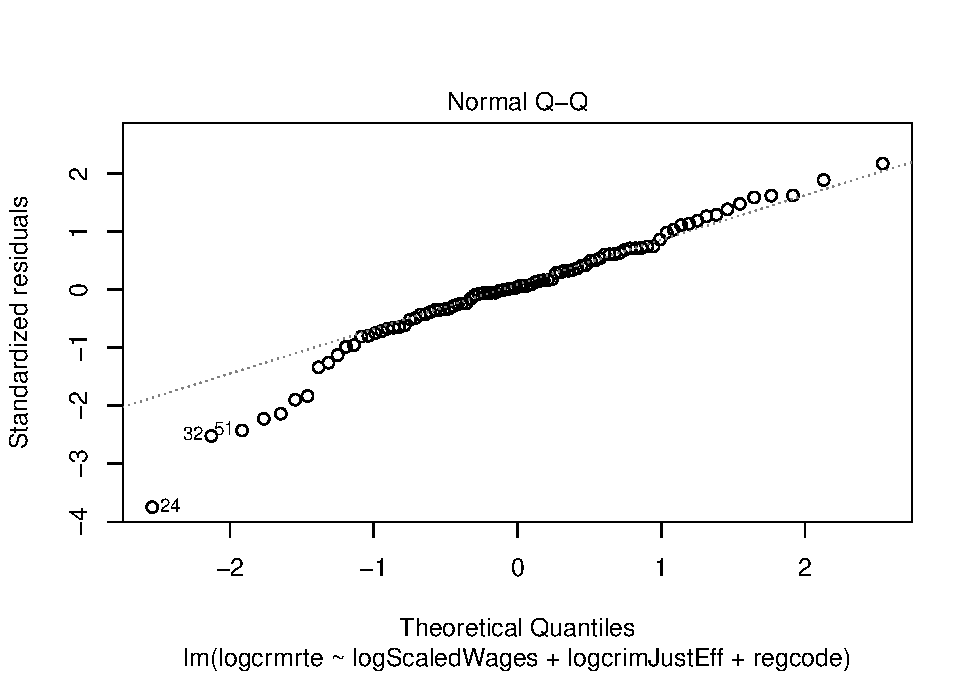
\includegraphics{Bagnard_Gaustad_Hartman_Leung_Lab_3_files/figure-latex/unnamed-chunk-65-1.pdf}

\begin{Shaded}
\begin{Highlighting}[]
\NormalTok{dfCrime[dfCrime}\OperatorTok{$}\NormalTok{crimJustEff }\OperatorTok{>}\StringTok{ }\DecValTok{1}\NormalTok{,] }\CommentTok{# find outlier}
\end{Highlighting}
\end{Shaded}

\begin{verbatim}
   county year    crmrte  prbarr prbconv prbpris avgsen      polpc
51    115   87 0.0055332 1.09091     1.5     0.5   20.7 0.00905433
     density   taxpc west central urban  pctmin80     wcon     wtuc
51 0.3858093 28.1931    1       0     0 0.0128365 204.2206 503.2351
       wtrd     wfir     wser   wmfg  wfed   wsta   wloc mix    pctymle
51 217.4908 342.4658 245.2061 448.42 442.2 340.39 386.12 0.1 0.07253495
   region regcode other nonurban   metro  logwcon  logwtuc  logwtrd
51      1       W     0        1 Outside 5.319201 6.221057 5.382157
    logwfir  logwser logwmfg  logwfed  logwsta  logwloc  logprbarr
51 5.836172 5.502099 6.10573 6.091762 5.830092 5.956148 0.08701217
   logprbconv logprbpris logavgsen  logpolpc    logmix logdensity
51  0.4054651 -0.6931472  3.030134 -4.704512 -2.302585 -0.9524121
   logpctmin80 logpctymle logcrmrte logtaxpc allWages crimJustEff
51   -4.355463  -2.623687 -5.196989 3.339077 3129.748    1.636365
   logcrimJustEff
51      0.4924773
\end{verbatim}

We see that pbarr and prbconv are both \textgreater{} 1. This is not
possible because you cannot be convicted more than once for the same
offense. We have an issue with the probability ratios. We will use the
imputation method to replace their values and remove the outlier effect,
while also retaining the rest of the variables in the county.

We also see that polpc is .009. We noticed this outlier during our EDA
analysis. Based on the records describing the US population on police
officers per capita, the highest police per capita on record is .007 in
Atlantic City, NJ.
\url{https://www.governing.com/gov-data/safety-justice/police-officers-per-capita-rates-employment-for-city-departments.html}
This datapoint is also in error and we will impute it's replacement.

\begin{Shaded}
\begin{Highlighting}[]
\NormalTok{dfCrime}\OperatorTok{$}\NormalTok{prbarr[}\KeywordTok{which}\NormalTok{(dfCrime}\OperatorTok{$}\NormalTok{county}\OperatorTok{==}\DecValTok{115}\NormalTok{)]<-}\OtherTok{NA} \CommentTok{# set the value to NA so it will be imputed}
\NormalTok{dfCrime}\OperatorTok{$}\NormalTok{prbconv[}\KeywordTok{which}\NormalTok{(dfCrime}\OperatorTok{$}\NormalTok{county}\OperatorTok{==}\DecValTok{115}\NormalTok{)]<-}\OtherTok{NA} \CommentTok{# set the value to NA so it will be imputed}
\NormalTok{dfCrime}\OperatorTok{$}\NormalTok{polpc[}\KeywordTok{which}\NormalTok{(dfCrime}\OperatorTok{$}\NormalTok{county}\OperatorTok{==}\DecValTok{115}\NormalTok{)]<-}\OtherTok{NA} \CommentTok{# set the value to NA so it will be imputed}
\end{Highlighting}
\end{Shaded}

\begin{Shaded}
\begin{Highlighting}[]
\NormalTok{impute_arg <-}\StringTok{ }\KeywordTok{aregImpute}\NormalTok{(}\OperatorTok{~}\StringTok{ }\NormalTok{crmrte }\OperatorTok{+}\StringTok{  }\NormalTok{urban }\OperatorTok{+}\StringTok{ }\NormalTok{central }\OperatorTok{+}\StringTok{ }\NormalTok{west }\OperatorTok{+}\StringTok{ }\NormalTok{other }\OperatorTok{+}
\StringTok{                         }\NormalTok{prbarr }\OperatorTok{+}\StringTok{ }\NormalTok{prbconv }\OperatorTok{+}\StringTok{ }\NormalTok{prbpris }\OperatorTok{+}\StringTok{ }\NormalTok{avgsen }\OperatorTok{+}\StringTok{ }\NormalTok{polpc }\OperatorTok{+}\StringTok{ }
\StringTok{                         }\NormalTok{density }\OperatorTok{+}\StringTok{ }\NormalTok{taxpc }\OperatorTok{+}\StringTok{ }\NormalTok{pctmin80 }\OperatorTok{+}\StringTok{ }\NormalTok{wcon }\OperatorTok{+}\StringTok{ }\NormalTok{wtuc }\OperatorTok{+}
\StringTok{                         }\NormalTok{wtrd }\OperatorTok{+}\StringTok{ }\NormalTok{wfir }\OperatorTok{+}\StringTok{ }\NormalTok{wser }\OperatorTok{+}\StringTok{ }\NormalTok{wmfg }\OperatorTok{+}\StringTok{ }\NormalTok{wfed }\OperatorTok{+}\StringTok{ }\NormalTok{wsta }\OperatorTok{+}\StringTok{ }\NormalTok{wloc }\OperatorTok{+}
\StringTok{                         }\NormalTok{mix }\OperatorTok{+}\StringTok{ }\NormalTok{pctymle, }\DataTypeTok{data =}\NormalTok{ dfCrime, }\DataTypeTok{match=}\StringTok{"weighted"}\NormalTok{,}
                         \DataTypeTok{nk=}\DecValTok{3}\NormalTok{, }\DataTypeTok{B=}\DecValTok{10}\NormalTok{, }\DataTypeTok{n.impute =} \DecValTok{100}\NormalTok{)}
\end{Highlighting}
\end{Shaded}

\begin{Shaded}
\begin{Highlighting}[]
\KeywordTok{paste}\NormalTok{(}\StringTok{"R-squares for Predicting Non-Missing Values for Each Variable"}\NormalTok{)}
\end{Highlighting}
\end{Shaded}

\begin{verbatim}
[1] "R-squares for Predicting Non-Missing Values for Each Variable"
\end{verbatim}

\begin{Shaded}
\begin{Highlighting}[]
\NormalTok{impute_arg}\OperatorTok{$}\NormalTok{rsq}
\end{Highlighting}
\end{Shaded}

\begin{verbatim}
   prbarr   prbconv     polpc 
0.9155074 0.9269223 0.9068329 
\end{verbatim}

\begin{Shaded}
\begin{Highlighting}[]
\KeywordTok{paste}\NormalTok{(}\StringTok{"Distribution of Values for Each Imputation"}\NormalTok{)}
\end{Highlighting}
\end{Shaded}

\begin{verbatim}
[1] "Distribution of Values for Each Imputation"
\end{verbatim}

\begin{Shaded}
\begin{Highlighting}[]
\KeywordTok{table}\NormalTok{(impute_arg}\OperatorTok{$}\NormalTok{imputed}\OperatorTok{$}\NormalTok{prbarr)}
\end{Highlighting}
\end{Shaded}

\begin{verbatim}

0.092770003 0.132028997 0.133224994 0.146132007 0.153845996 0.162860006 
          1           2           1           1           1           1 
0.175649002 0.190876007 0.195265993 0.204216003 0.207142994 0.217215002 
          1           1           1           2           1           1 
0.221542001    0.222002 0.236600995 0.243589997 0.264420003 0.266054988 
          1           1           1           1           1           2 
0.269042999  0.27094999 0.271966994 0.278286994 0.296645999 0.298269987 
          2           2           2           1           1          32 
0.300215006 0.310986996 0.323547989  0.33266899 0.338901997  0.34067899 
          1           2           2           2           1           1 
0.343073994 0.364760011 0.381399989 0.392111003 0.408199996 0.444444001 
          3           3           2           3           3           2 
0.518218994 0.522696018 0.530435026 0.689023972 
          1           3           3           7 
\end{verbatim}

\begin{Shaded}
\begin{Highlighting}[]
\KeywordTok{paste}\NormalTok{(}\StringTok{"Distribution of Values for Each Imputation"}\NormalTok{)}
\end{Highlighting}
\end{Shaded}

\begin{verbatim}
[1] "Distribution of Values for Each Imputation"
\end{verbatim}

\begin{Shaded}
\begin{Highlighting}[]
\KeywordTok{table}\NormalTok{(impute_arg}\OperatorTok{$}\NormalTok{imputed}\OperatorTok{$}\NormalTok{prbconv)}
\end{Highlighting}
\end{Shaded}

\begin{verbatim}

0.226361006 0.259833008 0.267856985 0.327868998 0.328664005 0.340490997 
          1           1           2           1           1           1 
0.343023002 0.384236008    0.401198 0.403780013 0.410596013 0.412698001 
          1           1           1           1           1           1 
0.443681002 0.452829987 0.477732986 0.515464008 0.527595997 0.528302014 
          1           1           1           1          20           1 
0.549019992 0.559822977  0.62251699 0.736908972 0.739394009 0.763333023 
          1           1           1           3           1           2 
0.769231021 0.781608999 0.909090996 0.972972989 1.068969965 1.182929993 
          1           4           2           2           3           1 
1.225610018 1.234380007 1.358139992 1.481480002 1.670519948 2.121210098 
          3           5           1           3          14          14 
\end{verbatim}

\begin{Shaded}
\begin{Highlighting}[]
\KeywordTok{paste}\NormalTok{(}\StringTok{"Distribution of Values for Each Imputation"}\NormalTok{)}
\end{Highlighting}
\end{Shaded}

\begin{verbatim}
[1] "Distribution of Values for Each Imputation"
\end{verbatim}

\begin{Shaded}
\begin{Highlighting}[]
\KeywordTok{table}\NormalTok{(impute_arg}\OperatorTok{$}\NormalTok{imputed}\OperatorTok{$}\NormalTok{polpc)}
\end{Highlighting}
\end{Shaded}

\begin{verbatim}

0.00074588 0.00075593 0.00081426 0.00085438 0.00086018 0.00108043 
         1          1          6          2          3          3 
0.00122733 0.00123431 0.00124824 0.00126447 0.00129761  0.0013704 
         1          1          1          1          3          1 
0.00138447  0.0014373 0.00145925 0.00148532   0.001516 0.00151871 
         1          2          1          1          1          1 
0.00154457 0.00167448 0.00168747  0.0016918 0.00182786 0.00182958 
         1          3          2          2         29          1 
0.00185912 0.00189444 0.00190802 0.00195614  0.0019714 0.00202425 
         1          2          2          1          2          1 
0.00207028 0.00217747 0.00227837 0.00233871 0.00243562 0.00255849 
         3          1          1          2          1          1 
0.00288203 0.00400962 0.00445923 
         1          4          8 
\end{verbatim}

We will reassign the value in our dataset to the mean from these trials.

\begin{Shaded}
\begin{Highlighting}[]
\NormalTok{dfCrime}\OperatorTok{$}\NormalTok{prbarr[}\KeywordTok{which}\NormalTok{(dfCrime}\OperatorTok{$}\NormalTok{county}\OperatorTok{==}\DecValTok{115}\NormalTok{)]<-}\KeywordTok{mean}\NormalTok{(impute_arg}\OperatorTok{$}\NormalTok{imputed}\OperatorTok{$}\NormalTok{prbarr)}
\NormalTok{dfCrime}\OperatorTok{$}\NormalTok{prbarr[}\KeywordTok{which}\NormalTok{(dfCrime}\OperatorTok{$}\NormalTok{county}\OperatorTok{==}\DecValTok{115}\NormalTok{)]}
\end{Highlighting}
\end{Shaded}

\begin{verbatim}
[1] 0.3340234
\end{verbatim}

\begin{Shaded}
\begin{Highlighting}[]
\NormalTok{dfCrime}\OperatorTok{$}\NormalTok{prbconv[}\KeywordTok{which}\NormalTok{(dfCrime}\OperatorTok{$}\NormalTok{county}\OperatorTok{==}\DecValTok{115}\NormalTok{)]<-}\KeywordTok{mean}\NormalTok{(impute_arg}\OperatorTok{$}\NormalTok{imputed}\OperatorTok{$}\NormalTok{prbconv)}
\NormalTok{dfCrime}\OperatorTok{$}\NormalTok{prbconv[}\KeywordTok{which}\NormalTok{(dfCrime}\OperatorTok{$}\NormalTok{county}\OperatorTok{==}\DecValTok{115}\NormalTok{)]}
\end{Highlighting}
\end{Shaded}

\begin{verbatim}
[1] 1.043377
\end{verbatim}

\begin{Shaded}
\begin{Highlighting}[]
\NormalTok{dfCrime}\OperatorTok{$}\NormalTok{polpc[}\KeywordTok{which}\NormalTok{(dfCrime}\OperatorTok{$}\NormalTok{county}\OperatorTok{==}\DecValTok{115}\NormalTok{)]<-}\KeywordTok{mean}\NormalTok{(impute_arg}\OperatorTok{$}\NormalTok{imputed}\OperatorTok{$}\NormalTok{polpc)}
\NormalTok{dfCrime}\OperatorTok{$}\NormalTok{polpc[}\KeywordTok{which}\NormalTok{(dfCrime}\OperatorTok{$}\NormalTok{county}\OperatorTok{==}\DecValTok{115}\NormalTok{)]}
\end{Highlighting}
\end{Shaded}

\begin{verbatim}
[1] 0.001948778
\end{verbatim}

\begin{Shaded}
\begin{Highlighting}[]
\NormalTok{dfCrime}\OperatorTok{$}\NormalTok{logprbarr[}\KeywordTok{which}\NormalTok{(dfCrime}\OperatorTok{$}\NormalTok{county}\OperatorTok{==}\DecValTok{115}\NormalTok{)]<-}\KeywordTok{log}\NormalTok{(dfCrime}\OperatorTok{$}\NormalTok{prbarr[}\KeywordTok{which}\NormalTok{(dfCrime}\OperatorTok{$}\NormalTok{county}\OperatorTok{==}\DecValTok{115}\NormalTok{)])}
\NormalTok{dfCrime}\OperatorTok{$}\NormalTok{logprbarr[}\KeywordTok{which}\NormalTok{(dfCrime}\OperatorTok{$}\NormalTok{county}\OperatorTok{==}\DecValTok{115}\NormalTok{)]}
\end{Highlighting}
\end{Shaded}

\begin{verbatim}
[1] -1.096544
\end{verbatim}

\begin{Shaded}
\begin{Highlighting}[]
\NormalTok{dfCrime}\OperatorTok{$}\NormalTok{logprbconv[}\KeywordTok{which}\NormalTok{(dfCrime}\OperatorTok{$}\NormalTok{county}\OperatorTok{==}\DecValTok{115}\NormalTok{)]<-}\KeywordTok{log}\NormalTok{(dfCrime}\OperatorTok{$}\NormalTok{prbconv[}\KeywordTok{which}\NormalTok{(dfCrime}\OperatorTok{$}\NormalTok{county}\OperatorTok{==}\DecValTok{115}\NormalTok{)])}
\NormalTok{dfCrime}\OperatorTok{$}\NormalTok{logprbconv[}\KeywordTok{which}\NormalTok{(dfCrime}\OperatorTok{$}\NormalTok{county}\OperatorTok{==}\DecValTok{115}\NormalTok{)]}
\end{Highlighting}
\end{Shaded}

\begin{verbatim}
[1] 0.04246262
\end{verbatim}

\begin{Shaded}
\begin{Highlighting}[]
\NormalTok{dfCrime}\OperatorTok{$}\NormalTok{logpolpc[}\KeywordTok{which}\NormalTok{(dfCrime}\OperatorTok{$}\NormalTok{county}\OperatorTok{==}\DecValTok{115}\NormalTok{)]<-}\KeywordTok{log}\NormalTok{(dfCrime}\OperatorTok{$}\NormalTok{polpc[}\KeywordTok{which}\NormalTok{(dfCrime}\OperatorTok{$}\NormalTok{county}\OperatorTok{==}\DecValTok{115}\NormalTok{)])}
\NormalTok{dfCrime}\OperatorTok{$}\NormalTok{logpolpc[}\KeywordTok{which}\NormalTok{(dfCrime}\OperatorTok{$}\NormalTok{county}\OperatorTok{==}\DecValTok{115}\NormalTok{)]}
\end{Highlighting}
\end{Shaded}

\begin{verbatim}
[1] -6.240553
\end{verbatim}

\begin{Shaded}
\begin{Highlighting}[]
\NormalTok{dfCrime}\OperatorTok{$}\NormalTok{crimJustEff<-dfCrime}\OperatorTok{$}\NormalTok{prbarr }\OperatorTok{*}\StringTok{ }\NormalTok{dfCrime}\OperatorTok{$}\NormalTok{prbconv}
\NormalTok{dfCrime}\OperatorTok{$}\NormalTok{logcrimJustEff<-}\KeywordTok{log}\NormalTok{(dfCrime}\OperatorTok{$}\NormalTok{crimJustEff)}
\end{Highlighting}
\end{Shaded}

\begin{Shaded}
\begin{Highlighting}[]
\KeywordTok{ggplot}\NormalTok{(}\DataTypeTok{data=}\NormalTok{dfCrime, }\KeywordTok{aes}\NormalTok{(}\DataTypeTok{sample=}\NormalTok{ crimJustEff)) }\OperatorTok{+}\StringTok{ }\KeywordTok{stat_qq}\NormalTok{() }\OperatorTok{+}\StringTok{ }\KeywordTok{stat_qq_line}\NormalTok{() }\OperatorTok{+}\StringTok{ }
\StringTok{  }\KeywordTok{ggtitle}\NormalTok{(}\StringTok{"QQ Plot of Crim Just Eff"}\NormalTok{)}
\end{Highlighting}
\end{Shaded}

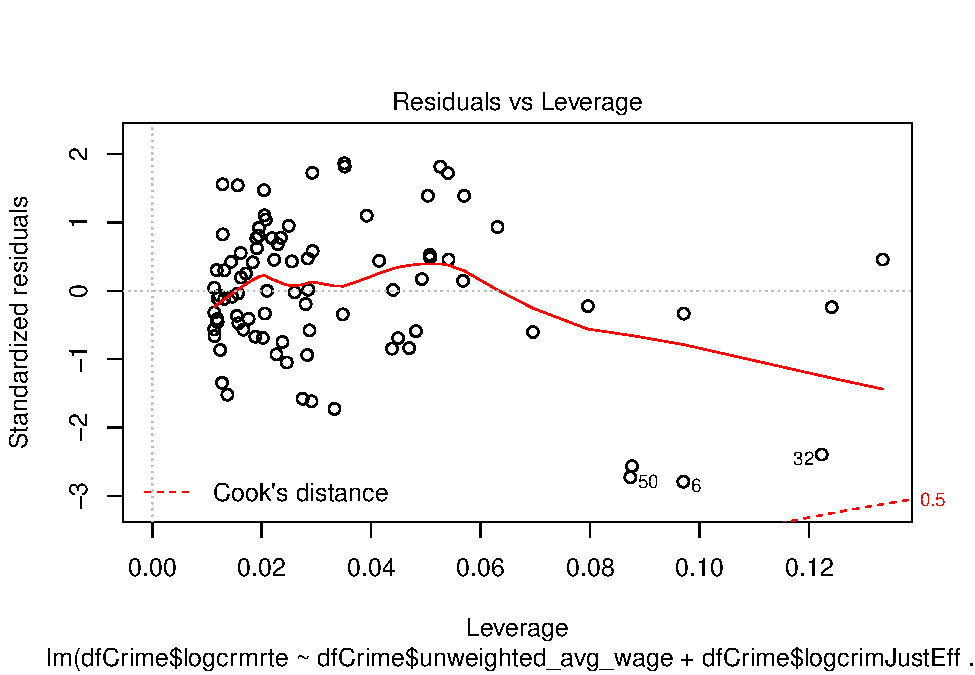
\includegraphics{Bagnard_Gaustad_Hartman_Leung_Lab_3_files/figure-latex/unnamed-chunk-76-1.pdf}

\begin{Shaded}
\begin{Highlighting}[]
\KeywordTok{ggplot}\NormalTok{(}\DataTypeTok{data=}\NormalTok{dfCrime, }\KeywordTok{aes}\NormalTok{(}\DataTypeTok{sample=}\NormalTok{ logcrimJustEff)) }\OperatorTok{+}\StringTok{ }\KeywordTok{stat_qq}\NormalTok{() }\OperatorTok{+}\StringTok{ }\KeywordTok{stat_qq_line}\NormalTok{() }\OperatorTok{+}\StringTok{ }
\KeywordTok{ggtitle}\NormalTok{(}\StringTok{"QQ Plot of log transformed Crim Just Eff"}\NormalTok{)}
\end{Highlighting}
\end{Shaded}

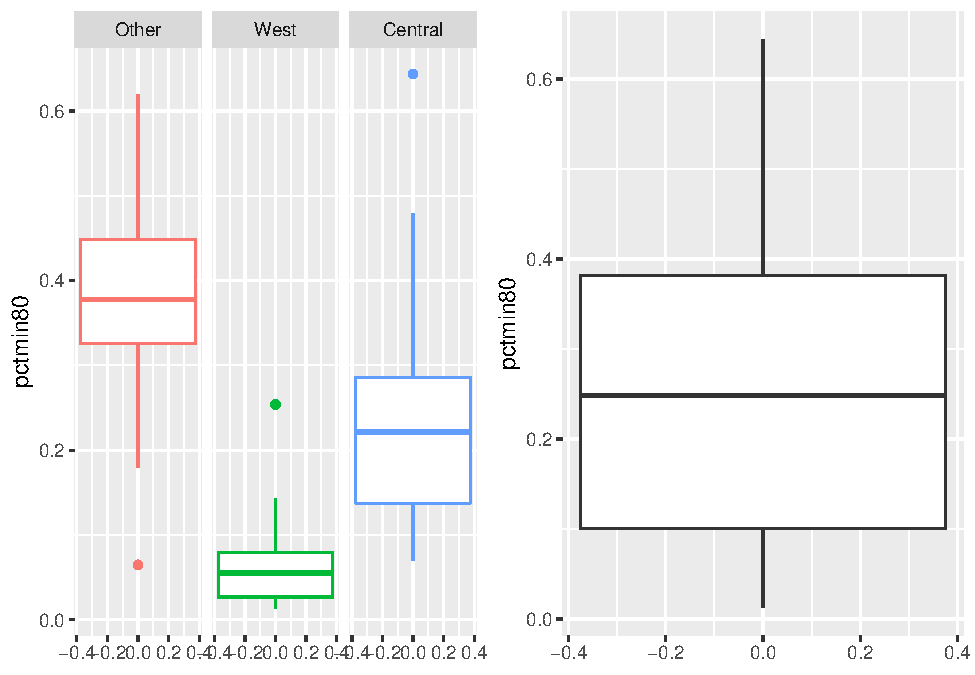
\includegraphics{Bagnard_Gaustad_Hartman_Leung_Lab_3_files/figure-latex/unnamed-chunk-77-1.pdf}

\begin{Shaded}
\begin{Highlighting}[]
\CommentTok{## Can show histogram/qqplot side by side in RMD. }
\end{Highlighting}
\end{Shaded}

We theorize that the second major cause of crime are bad economic
conditions. When there are worse economic conditions, crime can be more
attractive due to:

\begin{itemize}
\tightlist
\item
  Lack of means: People forced into crimes because they need to make
  ends meet
\item
  Lack of occupation: People commit crimes because they are not busy at
  work
\item
  Lack of opportunity: High discount rate for future due to no long-term
  opportunity, incentive to take the risk and commit crimes hoping for
  big payoff.
\end{itemize}

We operationalize economic conditions by looking at wages. For this
model, we define this as the sum of all average wages in each county. We
think this is best proxy from our data because it answers all of the
above (higher wages leads to better means and better opportunities).
From our EDA we also confirm that in general these sums are not skewed
by having 1 really high paying sector in each county as we see a strong
relationship between avg quartile across all job types and total sum.
This can be seen in the chart below.

\begin{Shaded}
\begin{Highlighting}[]
\CommentTok{# # Quantiles for all jobs}
\NormalTok{dfWage<-}\KeywordTok{mutate}\NormalTok{(dfCrime,}\DataTypeTok{qCon=}\KeywordTok{ntile}\NormalTok{(dfCrime}\OperatorTok{$}\NormalTok{wcon,}\DecValTok{4}\NormalTok{))}
\NormalTok{dfWage<-}\KeywordTok{mutate}\NormalTok{(dfWage,}\DataTypeTok{qTuc=}\KeywordTok{ntile}\NormalTok{(dfCrime}\OperatorTok{$}\NormalTok{wtuc,}\DecValTok{4}\NormalTok{))}
\NormalTok{dfWage<-}\KeywordTok{mutate}\NormalTok{(dfWage,}\DataTypeTok{qTrd=}\KeywordTok{ntile}\NormalTok{(dfCrime}\OperatorTok{$}\NormalTok{wtrd,}\DecValTok{4}\NormalTok{))}
\NormalTok{dfWage<-}\KeywordTok{mutate}\NormalTok{(dfWage,}\DataTypeTok{qFir=}\KeywordTok{ntile}\NormalTok{(dfCrime}\OperatorTok{$}\NormalTok{wfir,}\DecValTok{4}\NormalTok{))}
\NormalTok{dfWage<-}\KeywordTok{mutate}\NormalTok{(dfWage,}\DataTypeTok{qSer=}\KeywordTok{ntile}\NormalTok{(dfCrime}\OperatorTok{$}\NormalTok{wser,}\DecValTok{4}\NormalTok{))}
\NormalTok{dfWage<-}\KeywordTok{mutate}\NormalTok{(dfWage,}\DataTypeTok{qMfg=}\KeywordTok{ntile}\NormalTok{(dfCrime}\OperatorTok{$}\NormalTok{wmfg,}\DecValTok{4}\NormalTok{))}
\NormalTok{dfWage<-}\KeywordTok{mutate}\NormalTok{(dfWage,}\DataTypeTok{qFed=}\KeywordTok{ntile}\NormalTok{(dfCrime}\OperatorTok{$}\NormalTok{wfed,}\DecValTok{4}\NormalTok{))}
\NormalTok{dfWage<-}\KeywordTok{mutate}\NormalTok{(dfWage,}\DataTypeTok{qSta=}\KeywordTok{ntile}\NormalTok{(dfCrime}\OperatorTok{$}\NormalTok{wsta,}\DecValTok{4}\NormalTok{))}
\NormalTok{dfWage<-}\KeywordTok{mutate}\NormalTok{(dfWage,}\DataTypeTok{qLoc=}\KeywordTok{ntile}\NormalTok{(dfCrime}\OperatorTok{$}\NormalTok{wloc,}\DecValTok{4}\NormalTok{))}
\CommentTok{## Average quantile}
\NormalTok{dfWage}\OperatorTok{$}\NormalTok{qAvg=}\StringTok{ }\NormalTok{(dfWage}\OperatorTok{$}\NormalTok{qCon}\OperatorTok{+}\NormalTok{dfWage}\OperatorTok{$}\NormalTok{qTuc}\OperatorTok{+}\NormalTok{dfWage}\OperatorTok{$}\NormalTok{qTrd}\OperatorTok{+}\NormalTok{dfWage}\OperatorTok{$}\NormalTok{qFir}\OperatorTok{+}\NormalTok{dfWage}\OperatorTok{$}\NormalTok{qSer}\OperatorTok{+}\NormalTok{dfWage}\OperatorTok{$}\NormalTok{qMfg}\OperatorTok{+}
\StringTok{                }\NormalTok{dfWage}\OperatorTok{$}\NormalTok{qFed}\OperatorTok{+}\NormalTok{dfWage}\OperatorTok{$}\NormalTok{qSta}\OperatorTok{+}\NormalTok{dfWage}\OperatorTok{$}\NormalTok{qLoc)}\OperatorTok{/}\DecValTok{9}
\KeywordTok{plot}\NormalTok{(dfCrime}\OperatorTok{$}\NormalTok{allWages,dfWage}\OperatorTok{$}\NormalTok{qAvg)}
\end{Highlighting}
\end{Shaded}

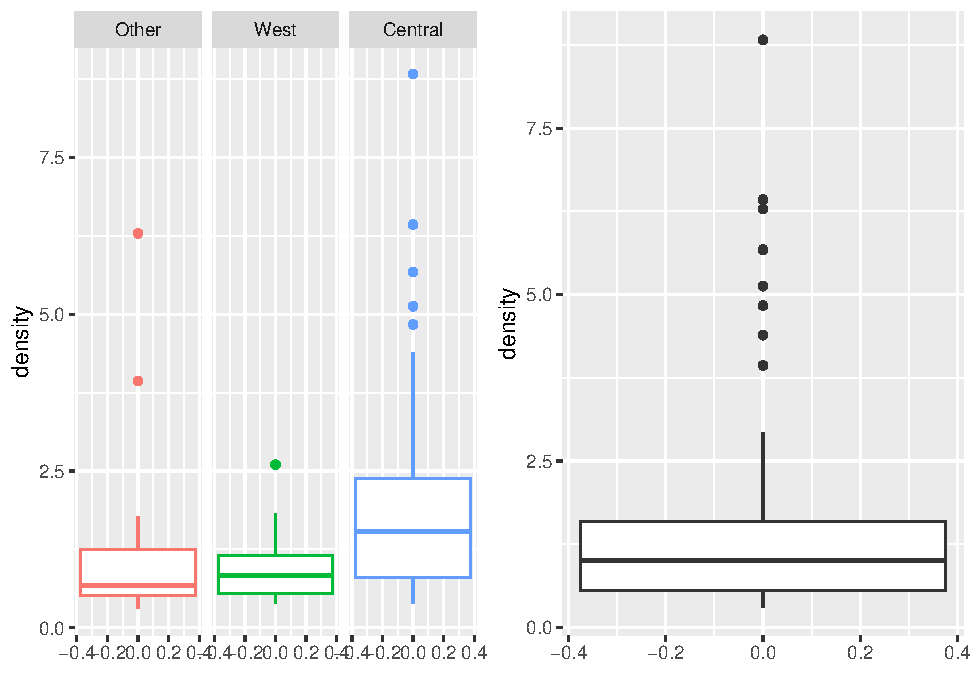
\includegraphics{Bagnard_Gaustad_Hartman_Leung_Lab_3_files/figure-latex/unnamed-chunk-78-1.pdf}

\begin{Shaded}
\begin{Highlighting}[]
\KeywordTok{hist}\NormalTok{(dfCrime}\OperatorTok{$}\NormalTok{allWages)}
\end{Highlighting}
\end{Shaded}

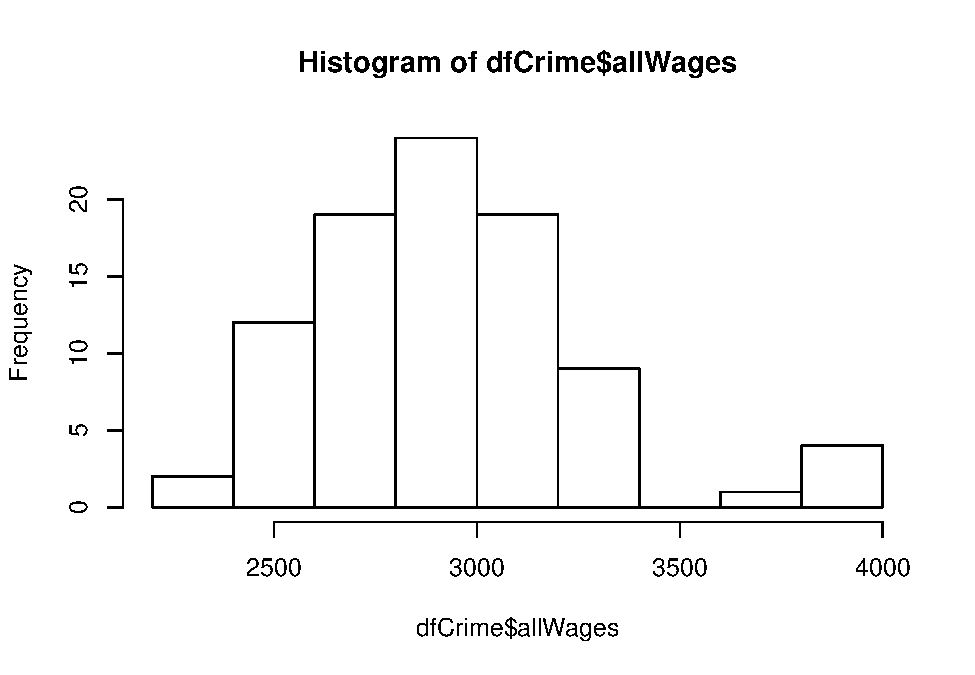
\includegraphics{Bagnard_Gaustad_Hartman_Leung_Lab_3_files/figure-latex/unnamed-chunk-79-1.pdf}

\begin{Shaded}
\begin{Highlighting}[]
\KeywordTok{ggplot}\NormalTok{(}\DataTypeTok{data=}\NormalTok{dfCrime, }\KeywordTok{aes}\NormalTok{(}\DataTypeTok{sample=}\NormalTok{ allWages)) }\OperatorTok{+}\StringTok{ }\KeywordTok{stat_qq}\NormalTok{() }\OperatorTok{+}\StringTok{ }\KeywordTok{stat_qq_line}\NormalTok{() }\OperatorTok{+}
\StringTok{  }\KeywordTok{ggtitle}\NormalTok{(}\StringTok{"QQ Plot of sum of wages"}\NormalTok{)}
\end{Highlighting}
\end{Shaded}

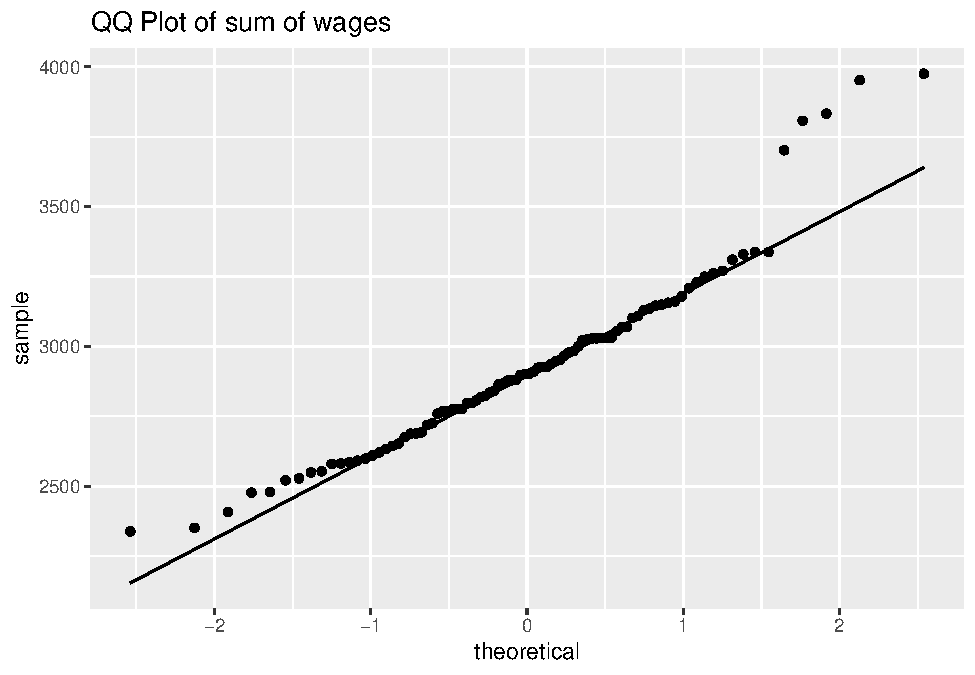
\includegraphics{Bagnard_Gaustad_Hartman_Leung_Lab_3_files/figure-latex/unnamed-chunk-79-2.pdf}

\hypertarget{model-1-linear-model}{%
\subsubsection{Model 1 Linear Model}\label{model-1-linear-model}}

\begin{Shaded}
\begin{Highlighting}[]
\NormalTok{dfCrime}\OperatorTok{$}\NormalTok{unweighted_avg_wage <-}\StringTok{ }\NormalTok{dfCrime}\OperatorTok{$}\NormalTok{allWages}\OperatorTok{/}\DecValTok{9}
\NormalTok{mod1 <-}\StringTok{ }\KeywordTok{lm}\NormalTok{(dfCrime}\OperatorTok{$}\NormalTok{logcrmrte }\OperatorTok{~}\StringTok{ }\NormalTok{dfCrime}\OperatorTok{$}\NormalTok{unweighted_avg_wage }\OperatorTok{+}\StringTok{ }\NormalTok{dfCrime}\OperatorTok{$}\NormalTok{logcrimJustEff)}
\KeywordTok{coeftest}\NormalTok{(mod1, }\DataTypeTok{vcov=}\NormalTok{vcovHC)}
\end{Highlighting}
\end{Shaded}

\begin{verbatim}

t test of coefficients:

                              Estimate Std. Error  t value  Pr(>|t|)    
(Intercept)                 -6.2847383  0.3703326 -16.9705 < 2.2e-16 ***
dfCrime$unweighted_avg_wage  0.0053015  0.0016175   3.2776 0.0015056 ** 
dfCrime$logcrimJustEff      -0.4892657  0.1314633  -3.7217 0.0003503 ***
---
Signif. codes:  0 '***' 0.001 '**' 0.01 '*' 0.05 '.' 0.1 ' ' 1
\end{verbatim}

\begin{Shaded}
\begin{Highlighting}[]
\KeywordTok{vif}\NormalTok{(mod1)}
\end{Highlighting}
\end{Shaded}

\begin{verbatim}
dfCrime$unweighted_avg_wage      dfCrime$logcrimJustEff 
                   1.053035                    1.053035 
\end{verbatim}

\begin{Shaded}
\begin{Highlighting}[]
\KeywordTok{summary}\NormalTok{(mod1)}\OperatorTok{$}\NormalTok{adj.r.square}
\end{Highlighting}
\end{Shaded}

\begin{verbatim}
[1] 0.4468565
\end{verbatim}

\begin{Shaded}
\begin{Highlighting}[]
\KeywordTok{shapiro.test}\NormalTok{(mod1}\OperatorTok{$}\NormalTok{residuals)}
\end{Highlighting}
\end{Shaded}

\begin{verbatim}

    Shapiro-Wilk normality test

data:  mod1$residuals
W = 0.95638, p-value = 0.004232
\end{verbatim}

The model gives estimates and standard errors that are heteroskedastic
consistent. The coefficient of unweighted\_avg\_wage is calculated to
have a coefficient of .005. This means that an increase of \$100 in
weekly wages is correlated with an increase of .5\% in crime rate.
Generally increased wages are not associated with increased crime. This
suggests that wages are correlated with a stronger omitted variable that
affects crime.

Similarly, criminal justice effectiveness (convictions/crime) is given a
coefficient of -0.489 which suggests that an increase 1\% increase in
convictions per crime is will decrease crime by nearly .5\%. This
suggests that we have found a are strong correlation and perhaps a good
influence on crime rate in a county.

\begin{Shaded}
\begin{Highlighting}[]
\KeywordTok{plot}\NormalTok{(mod1, }\DataTypeTok{which=}\DecValTok{5}\NormalTok{)}
\end{Highlighting}
\end{Shaded}

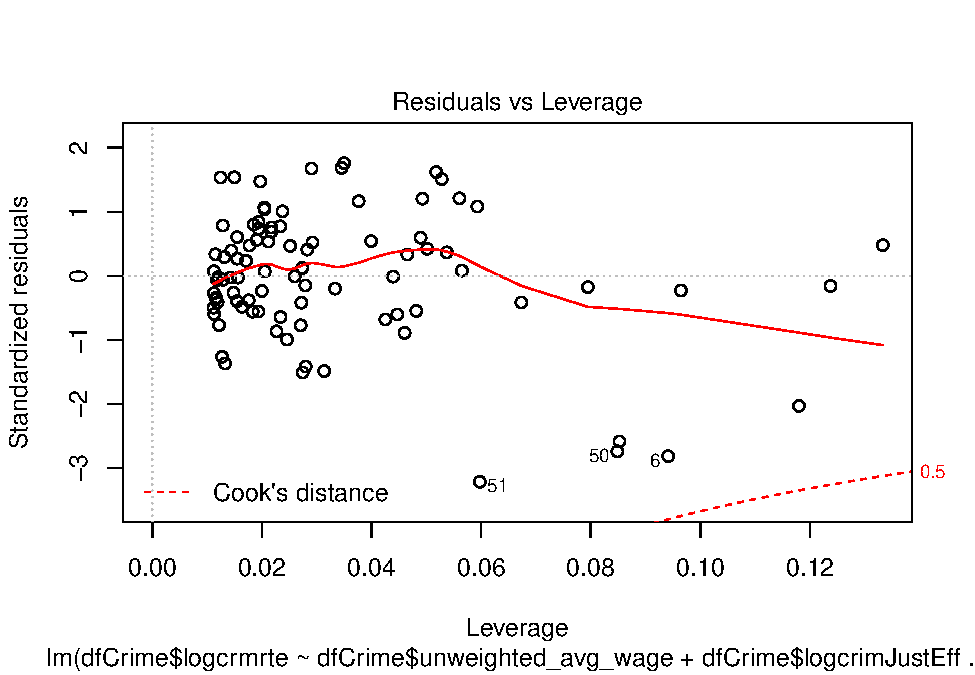
\includegraphics{Bagnard_Gaustad_Hartman_Leung_Lab_3_files/figure-latex/unnamed-chunk-81-1.pdf}

\begin{Shaded}
\begin{Highlighting}[]
\KeywordTok{plot}\NormalTok{(mod1, }\DataTypeTok{which=}\DecValTok{2}\NormalTok{)}
\end{Highlighting}
\end{Shaded}

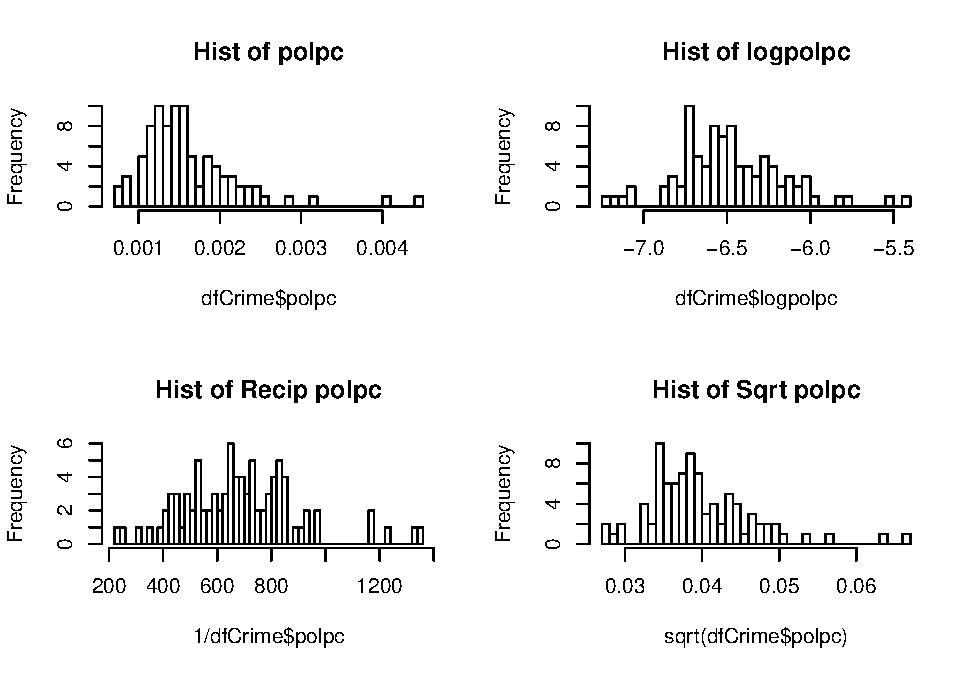
\includegraphics{Bagnard_Gaustad_Hartman_Leung_Lab_3_files/figure-latex/unnamed-chunk-82-1.pdf}

\begin{Shaded}
\begin{Highlighting}[]
\KeywordTok{plot}\NormalTok{(mod1, }\DataTypeTok{which=}\DecValTok{3}\NormalTok{)}
\end{Highlighting}
\end{Shaded}

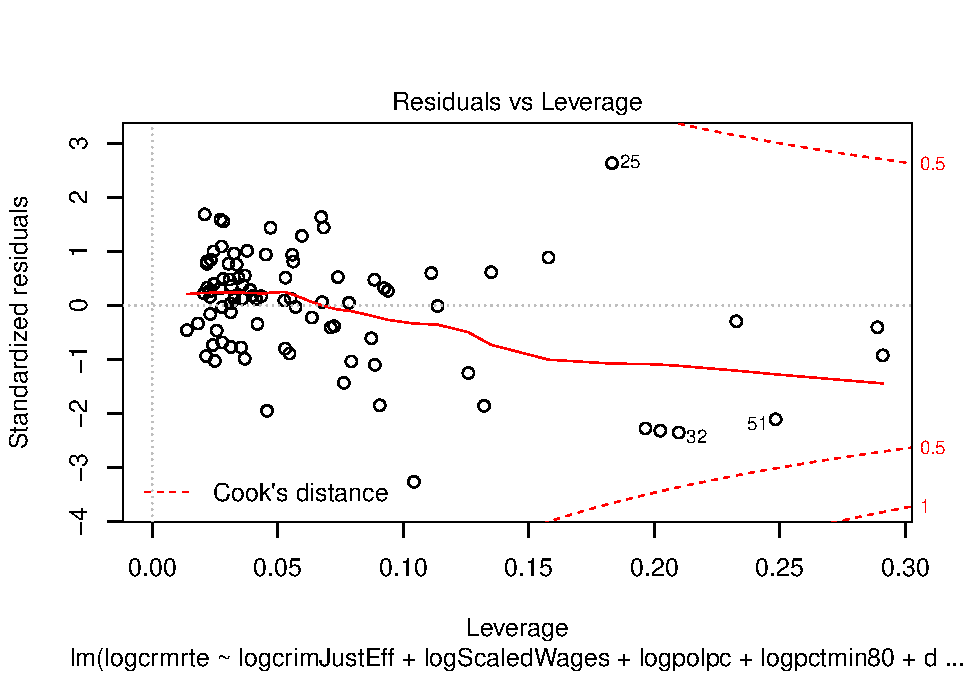
\includegraphics{Bagnard_Gaustad_Hartman_Leung_Lab_3_files/figure-latex/unnamed-chunk-83-1.pdf}

\begin{Shaded}
\begin{Highlighting}[]
\KeywordTok{plot}\NormalTok{(mod1, }\DataTypeTok{which=}\DecValTok{1}\NormalTok{)}
\end{Highlighting}
\end{Shaded}

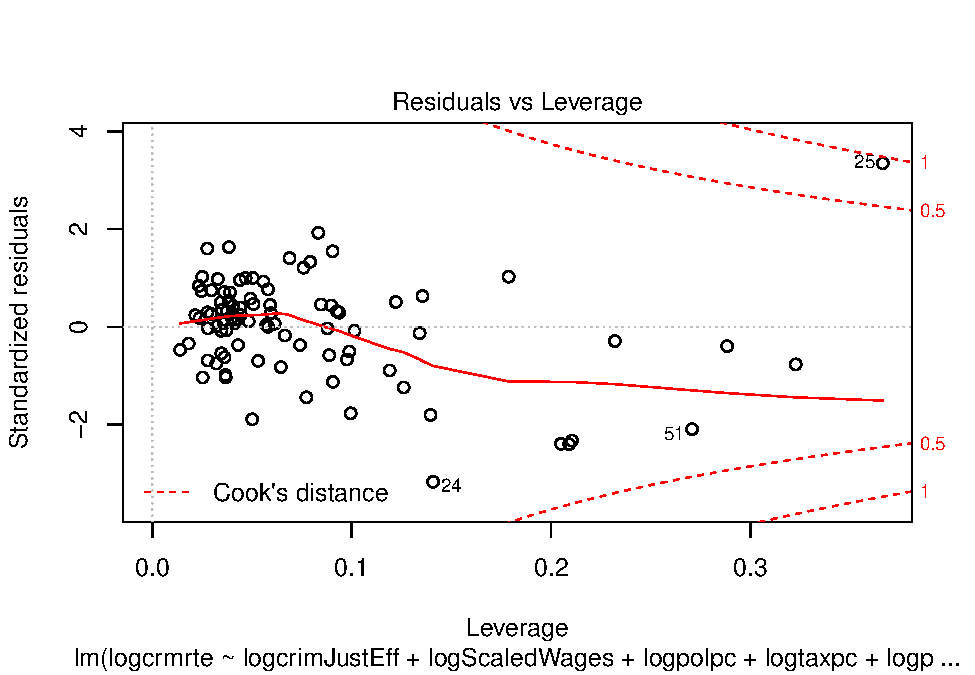
\includegraphics{Bagnard_Gaustad_Hartman_Leung_Lab_3_files/figure-latex/unnamed-chunk-84-1.pdf}

The model shows a moderate good fit, with an adjusted R square of 0.46.
This can be interpreted as, the model explains 46\% of the variation in
crime. Next the model is plotted in a Residuals vs Leverage plot. This
plot shows that all the points have a cook's distance of less than 0.5.
There are no points that have enough leverage and residual than when
deleted greatly alter the model coefficients.

The root of standardized residuals all fall within about 1.6. This is
very good, as we can expect 95\% of the points to fall within 3
standardized residuals of each other. (\(\sqrt(3) \approx 1.73\))

Finally, the residuals vs fitted plot shows a well centered and mostly
nromal distribution about 0. There are no major trends or variation
changes across the fitted values. This suggests that major uncorrelated
variables have not been left out of the model. We will discuss the
possible ommited variable biases further, in the next sections.

\textbf{Model 1 CLM Assumptions: {[}To be finalized{]}} * \textbf{MLR1}
Linear in paramters: The model has had its data transformed as described
above to allow a linear fit of the model. * \textbf{MLR2} Random
Sampling: The data is collected from a data set with rolled up data for
each county. It is not randomly sampled by area or population. *
\textbf{MLR3} No perfect multicollinearity: None of the variables chosen
for the model are constant or perfectly collinear as the economy and
criminal justice effectiveness are independent. * \textbf{MLR4'} The
expectation of u and and covariance of each regressor with u are
\textasciitilde{}0. This shows that our model's regressors are exogenous
with the error.\\
* \textbf{MLR4} The zero conditional mean assumption is well supported
when viewing the Residuals vs fitted plot. The split fit is nearly flat
and centered at 0. * \textbf{MLR5} There does appear to be
heteroskedacity in the `lips' appearance of the Residuals vs fitted
plot. This is acknowledged and can be accounted for by using the
heteroskedastic robust standard errors. This is seen in the coeftest. *
\textbf{MLR6} The final assumption of linear regression is that the
errors are normall distributed. This appears to hold for the bulk of the
residuals with some skewness in the tails. This is shown in the
significant return on the shapiro test. The model should not be used
when predicting crime rate for counties with extreme criminal justice
effectiveness or wages.

To summarize the value of model 1 we found a strong predictor in the
form of criminal justice effectiveness while wages are not good
predictors.

\begin{Shaded}
\begin{Highlighting}[]
\KeywordTok{cov}\NormalTok{(}\KeywordTok{resid}\NormalTok{(mod1), dfCrime}\OperatorTok{$}\NormalTok{allWages)}
\end{Highlighting}
\end{Shaded}

\begin{verbatim}
[1] -1.267354e-14
\end{verbatim}

\begin{Shaded}
\begin{Highlighting}[]
\KeywordTok{cov}\NormalTok{(}\KeywordTok{resid}\NormalTok{(mod1), }\KeywordTok{log}\NormalTok{(dfCrime}\OperatorTok{$}\NormalTok{crimJustEff))}
\end{Highlighting}
\end{Shaded}

\begin{verbatim}
[1] 1.983892e-17
\end{verbatim}

\begin{Shaded}
\begin{Highlighting}[]
\KeywordTok{mean}\NormalTok{(}\KeywordTok{resid}\NormalTok{(mod1))}
\end{Highlighting}
\end{Shaded}

\begin{verbatim}
[1] -9.474722e-19
\end{verbatim}

\hypertarget{model-2}{%
\subsection{Model 2}\label{model-2}}

\hypertarget{introduction-2}{%
\subsubsection{Introduction}\label{introduction-2}}

In this model, we introduce the additional covariates of population per
square mile (density), tax per capita (taxpc) and police per capita
(polpc) to increase the accuracy of our regression. We are including
these additional variables to our second model, as they add accuracy to
the explanatory variables used in our first model:

\begin{enumerate}
\def\labelenumi{\arabic{enumi}.}
\tightlist
\item
  The \textbf{Density} of an area can have significant impacts on:

  \begin{itemize}
  \tightlist
  \item
    \textbf{Criminal Justice Effectiveness}: with more people in a given
    area, crime frequency increases (+ bias direction). However, more
    people means there are more potential witnesses, making it easier to
    catch criminals (- bias direction).
  \item
    \textbf{Economic Opportunity (ie. AllWages)}: in high density areas,
    there is an increase in demand for support services such as food,
    retail, utilities, etc. As a result, there is a high demand for
    service jobs, which increases the economic opportunities within the
    area (+ bias direction). However, more people in a given area, there
    is a closer proximity to drugs, alcohol and gang violence - all of
    which are inhimitors to better economic outcomes.
  \end{itemize}
\item
  The \textbf{Police Per Capita} in a county can be influential on the
  Criminal Justice Effectiveness. With more police in a given area, one
  would think that crime rates would decrease, however our correlation
  plot below tells a different story. Including this variable in our
  analysis will give us more insight into the variables used in model 1.
\item
  The \textbf{Tax Per Capita} can have a direct impact on the Police Per
  Capita. A higher tax per capita, means that the county has more tax
  dollars to spend on protection services (ie. increasing the number of
  police in the county).
\end{enumerate}

\[log(crmrate) = \beta_0 + \beta_1crimjusteff + \beta_2log(polpc) + \beta_3density + \beta_4allWages + \beta_5taxpc + u\]

\hypertarget{model-2-eda-and-data-transformations}{%
\subsubsection{Model 2 EDA and Data
Transformations}\label{model-2-eda-and-data-transformations}}

\begin{Shaded}
\begin{Highlighting}[]
\KeywordTok{corrplot}\NormalTok{(}\KeywordTok{cor}\NormalTok{(dfCrime[,}\KeywordTok{c}\NormalTok{(}\StringTok{"logcrmrte"}\NormalTok{, }\StringTok{"logcrimJustEff"}\NormalTok{, }\StringTok{"logprbarr"}\NormalTok{, }\StringTok{"logprbconv"}\NormalTok{, }
                        \StringTok{"prbpris"}\NormalTok{, }\StringTok{"polpc"}\NormalTok{, }\StringTok{"taxpc"}\NormalTok{, }\StringTok{"allWages"}\NormalTok{, }\StringTok{"urban"}\NormalTok{, }\StringTok{"density"}\NormalTok{,}
                        \StringTok{"pctymle"}\NormalTok{, }\StringTok{"pctmin80"}\NormalTok{)]),}\DataTypeTok{method=}\StringTok{'circle'}\NormalTok{, }\DataTypeTok{type =} \StringTok{'lower'}\NormalTok{)}
\end{Highlighting}
\end{Shaded}

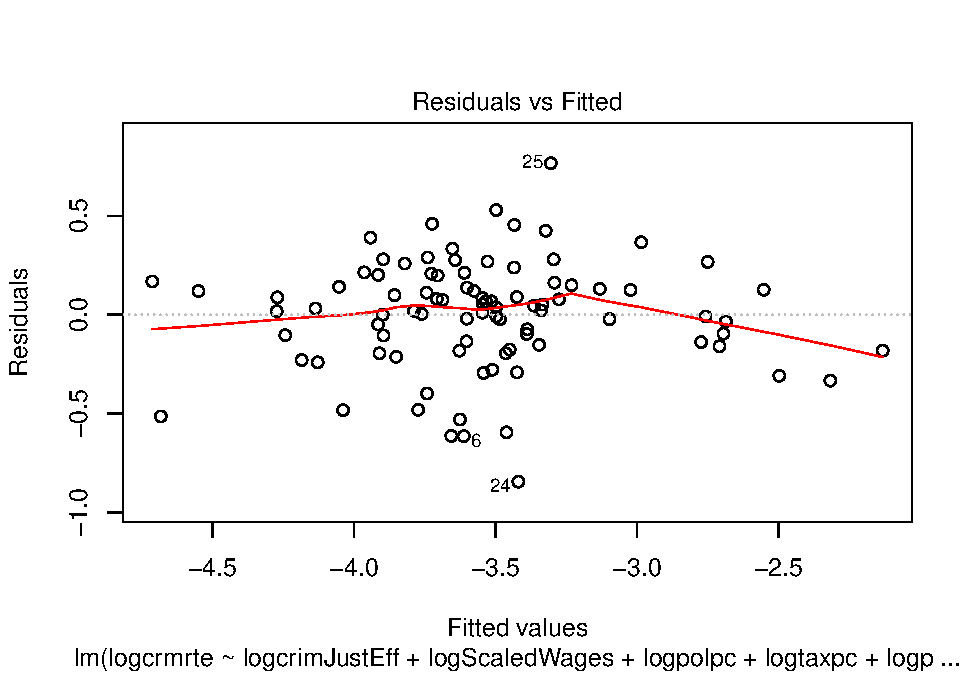
\includegraphics{Bagnard_Gaustad_Hartman_Leung_Lab_3_files/figure-latex/unnamed-chunk-86-1.pdf}

\begin{Shaded}
\begin{Highlighting}[]
\CommentTok{# polpc transformation analysis }
\KeywordTok{par}\NormalTok{(}\DataTypeTok{mfrow =} \KeywordTok{c}\NormalTok{(}\DecValTok{2}\NormalTok{,}\DecValTok{2}\NormalTok{))}
\KeywordTok{hist}\NormalTok{(dfCrime}\OperatorTok{$}\NormalTok{polpc, }\DataTypeTok{main=}\StringTok{"Hist of polpc"}\NormalTok{, }\DataTypeTok{breaks=}\DecValTok{50}\NormalTok{)}
\KeywordTok{hist}\NormalTok{(dfCrime}\OperatorTok{$}\NormalTok{logpolpc, }\DataTypeTok{main=}\StringTok{"Hist of logpolpc"}\NormalTok{, }\DataTypeTok{breaks=}\DecValTok{50}\NormalTok{)}
\KeywordTok{hist}\NormalTok{(}\DecValTok{1}\OperatorTok{/}\NormalTok{dfCrime}\OperatorTok{$}\NormalTok{polpc, }\DataTypeTok{main=}\StringTok{"Hist of Recip polpc"}\NormalTok{, }\DataTypeTok{breaks=}\DecValTok{50}\NormalTok{)}
\KeywordTok{hist}\NormalTok{(}\KeywordTok{sqrt}\NormalTok{(dfCrime}\OperatorTok{$}\NormalTok{polpc), }\DataTypeTok{main=}\StringTok{"Hist of Sqrt polpc"}\NormalTok{, }\DataTypeTok{breaks=}\DecValTok{50}\NormalTok{)}
\end{Highlighting}
\end{Shaded}

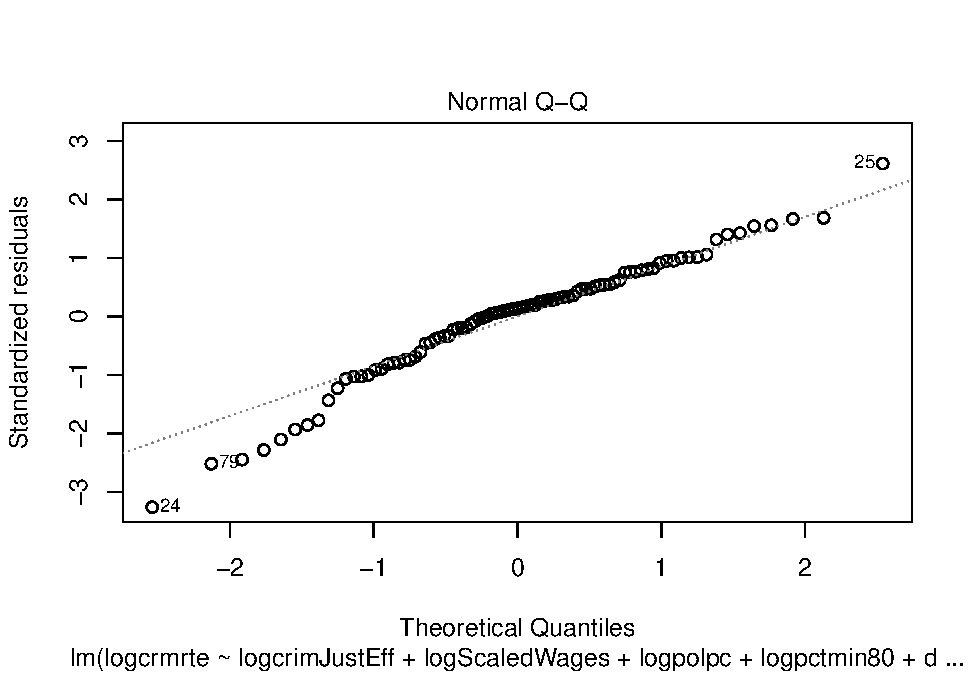
\includegraphics{Bagnard_Gaustad_Hartman_Leung_Lab_3_files/figure-latex/unnamed-chunk-87-1.pdf}

\begin{Shaded}
\begin{Highlighting}[]
\CommentTok{# taxpc transformation analysis }
\KeywordTok{par}\NormalTok{(}\DataTypeTok{mfrow =} \KeywordTok{c}\NormalTok{(}\DecValTok{2}\NormalTok{,}\DecValTok{2}\NormalTok{))}
\KeywordTok{hist}\NormalTok{(dfCrime}\OperatorTok{$}\NormalTok{taxpc, }\DataTypeTok{main=}\StringTok{"Hist of taxpc"}\NormalTok{, }\DataTypeTok{breaks=}\DecValTok{50}\NormalTok{)}
\KeywordTok{hist}\NormalTok{(dfCrime}\OperatorTok{$}\NormalTok{logtaxpc, }\DataTypeTok{main=}\StringTok{"Hist of logtaxpc"}\NormalTok{,}\DataTypeTok{breaks=}\DecValTok{50}\NormalTok{)}
\KeywordTok{hist}\NormalTok{(}\DecValTok{1}\OperatorTok{/}\NormalTok{dfCrime}\OperatorTok{$}\NormalTok{taxpc, }\DataTypeTok{main=}\StringTok{"Hist of Recip taxpc"}\NormalTok{, }\DataTypeTok{breaks=}\DecValTok{50}\NormalTok{)}
\KeywordTok{hist}\NormalTok{(}\KeywordTok{sqrt}\NormalTok{(dfCrime}\OperatorTok{$}\NormalTok{taxpc), }\DataTypeTok{main=}\StringTok{"Hist of Sqrt taxpc"}\NormalTok{, }\DataTypeTok{breaks=}\DecValTok{50}\NormalTok{)}
\end{Highlighting}
\end{Shaded}

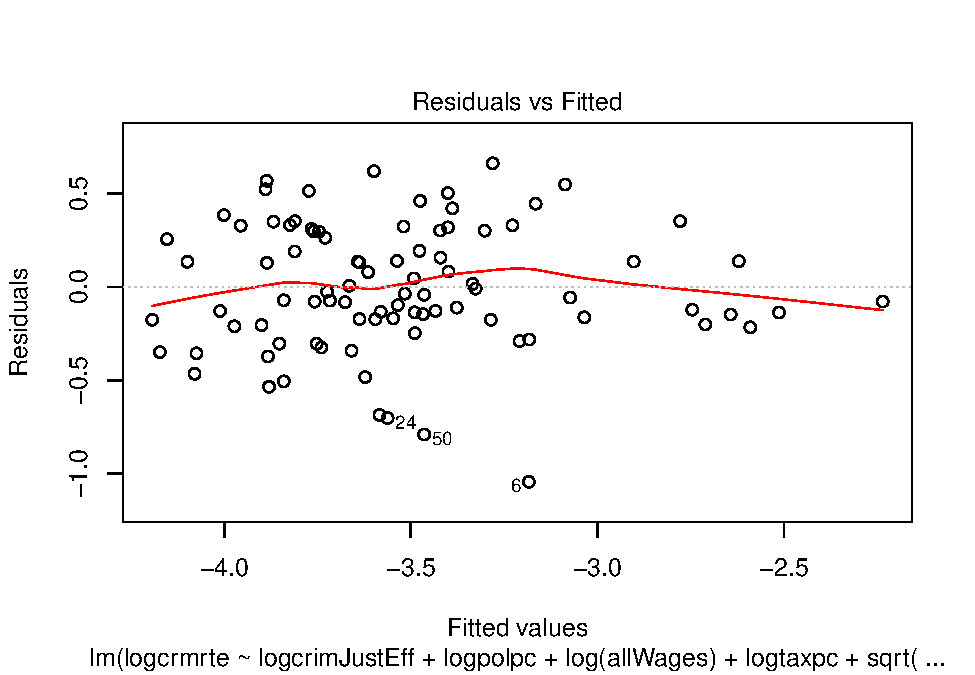
\includegraphics{Bagnard_Gaustad_Hartman_Leung_Lab_3_files/figure-latex/unnamed-chunk-88-1.pdf}

\begin{Shaded}
\begin{Highlighting}[]
\CommentTok{# density transformation analysis }
\KeywordTok{par}\NormalTok{(}\DataTypeTok{mfrow =} \KeywordTok{c}\NormalTok{(}\DecValTok{2}\NormalTok{,}\DecValTok{2}\NormalTok{))}
\KeywordTok{hist}\NormalTok{(dfCrime}\OperatorTok{$}\NormalTok{density, }\DataTypeTok{main=}\StringTok{"Hist of density"}\NormalTok{, }\DataTypeTok{breaks=}\DecValTok{50}\NormalTok{)}
\KeywordTok{hist}\NormalTok{(dfCrime}\OperatorTok{$}\NormalTok{logdensity, }\DataTypeTok{main=}\StringTok{"Hist of logdensity"}\NormalTok{,}\DataTypeTok{breaks=}\DecValTok{50}\NormalTok{)}
\KeywordTok{hist}\NormalTok{(}\DecValTok{1}\OperatorTok{/}\NormalTok{dfCrime}\OperatorTok{$}\NormalTok{density, }\DataTypeTok{main=}\StringTok{"Hist of Recip density"}\NormalTok{, }\DataTypeTok{breaks=}\DecValTok{50}\NormalTok{)}
\KeywordTok{hist}\NormalTok{(}\KeywordTok{sqrt}\NormalTok{(dfCrime}\OperatorTok{$}\NormalTok{density), }\DataTypeTok{main=}\StringTok{"Hist of Sqrt density"}\NormalTok{, }\DataTypeTok{breaks=}\DecValTok{50}\NormalTok{)}
\end{Highlighting}
\end{Shaded}

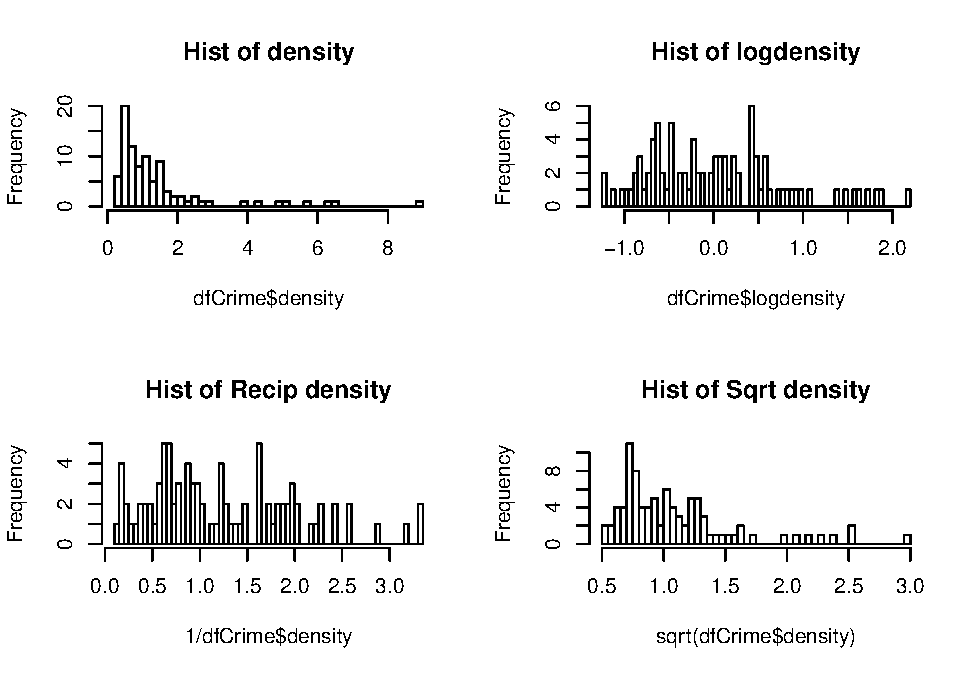
\includegraphics{Bagnard_Gaustad_Hartman_Leung_Lab_3_files/figure-latex/unnamed-chunk-89-1.pdf}

\begin{Shaded}
\begin{Highlighting}[]
\CommentTok{# par(mfrow = c(2,2))}
\CommentTok{# plot(dfCrime$logcrimJustEff, dfCrime$polpc, main = 'polpc vs logcrimJustEff', xlab='logcrimJustEff', ylab='polpc')}
\CommentTok{# plot(dfCrime$logcrimJustEff, dfCrime$logpolpc, main = 'logpolpc vs logcrimJustEff', xlab='logcrimJustEff', ylab='logpolpc')}
\CommentTok{# plot(dfCrime$logcrimJustEff, dfCrime$taxpc, main = 'taxpc vs logcrimJustEff', xlab='logcrimJustEff', ylab='taxpc')}
\CommentTok{# plot(dfCrime$logcrimJustEff, dfCrime$logtaxpc, main = 'logtaxpc vs logcrimJustEff', xlab='logcrimJustEff', ylab='logtaxpc')}
\end{Highlighting}
\end{Shaded}

-- AXLB - WIP

In the histograms above, we see that the both polpc and taxpc exhibit
right skew. Taking the natural log of polpc brings the distribution
closer to normal. However, the \(log\) of taxpc and density makes the
distributions even more skewed.

As a result, we will use the \(log\) of polpc (logpolpc) in our second
model and will not transform the taxpc and density variables.

\hypertarget{model-2-linear-model}{%
\subsubsection{Model 2 Linear Model}\label{model-2-linear-model}}

\begin{Shaded}
\begin{Highlighting}[]
\NormalTok{model2 <-}\StringTok{ }\KeywordTok{lm}\NormalTok{(logcrmrte }\OperatorTok{~}\StringTok{ }\NormalTok{logcrimJustEff }\OperatorTok{+}\StringTok{ }\NormalTok{logpolpc }\OperatorTok{+}\StringTok{ }\KeywordTok{log}\NormalTok{(allWages) }\OperatorTok{+}\StringTok{ }\NormalTok{logtaxpc }\OperatorTok{+}\StringTok{ }\KeywordTok{sqrt}\NormalTok{(dfCrime}\OperatorTok{$}\NormalTok{density), }\DataTypeTok{data =}\NormalTok{ dfCrime)}
\NormalTok{model2}
\end{Highlighting}
\end{Shaded}

\begin{verbatim}

Call:
lm(formula = logcrmrte ~ logcrimJustEff + logpolpc + log(allWages) + 
    logtaxpc + sqrt(dfCrime$density), data = dfCrime)

Coefficients:
          (Intercept)         logcrimJustEff               logpolpc  
              -5.0847                -0.2999                 0.2365  
        log(allWages)               logtaxpc  sqrt(dfCrime$density)  
               0.1862                 0.1228                 0.4778  
\end{verbatim}

\begin{Shaded}
\begin{Highlighting}[]
\KeywordTok{plot}\NormalTok{(model2)}
\end{Highlighting}
\end{Shaded}

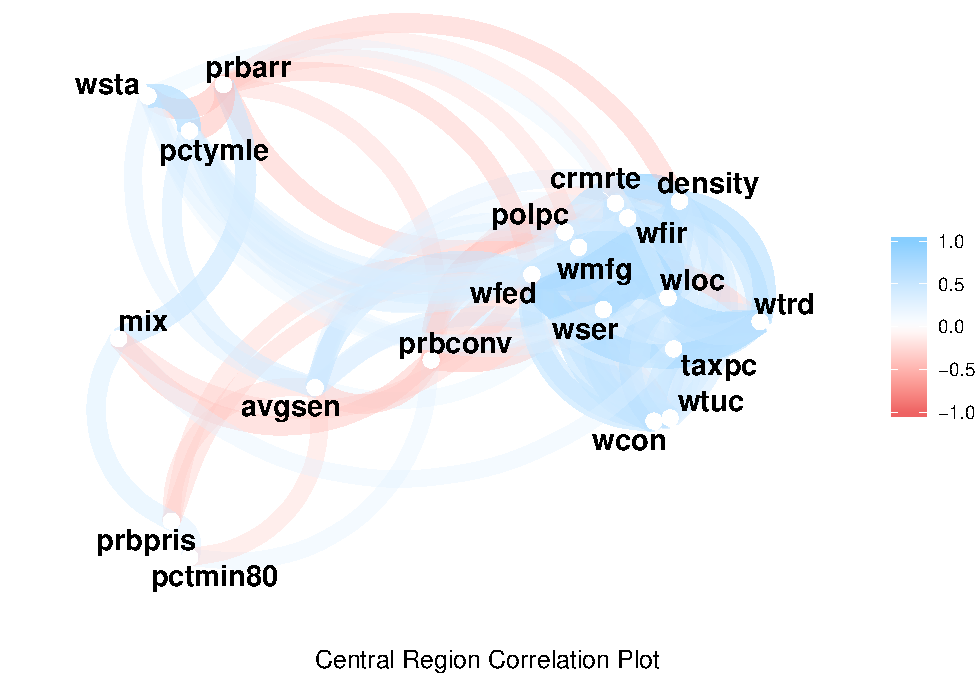
\includegraphics{Bagnard_Gaustad_Hartman_Leung_Lab_3_files/figure-latex/unnamed-chunk-91-1.pdf}
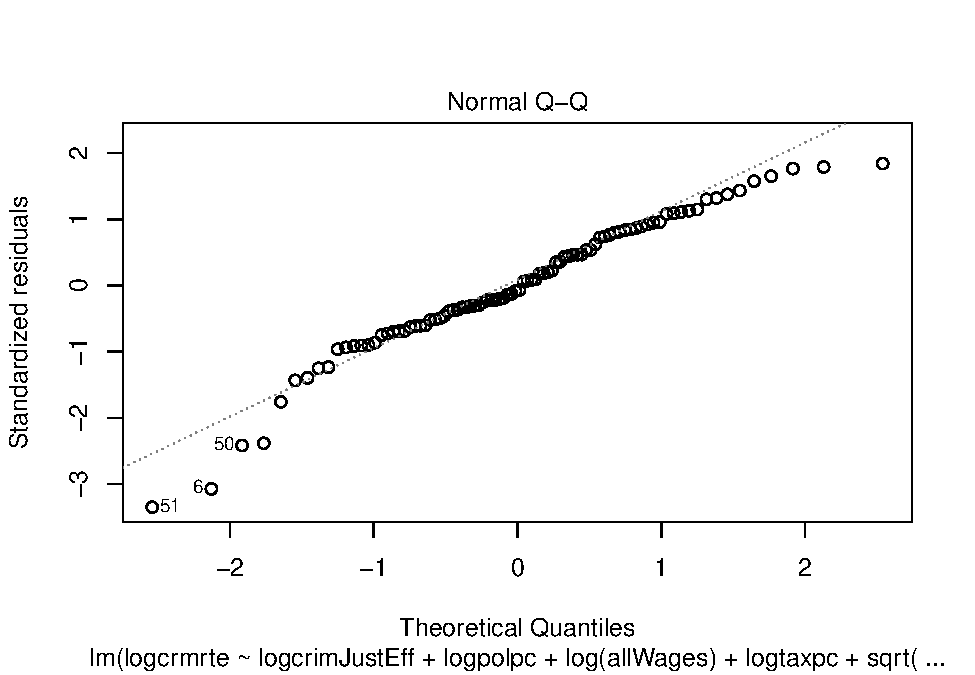
\includegraphics{Bagnard_Gaustad_Hartman_Leung_Lab_3_files/figure-latex/unnamed-chunk-91-2.pdf}
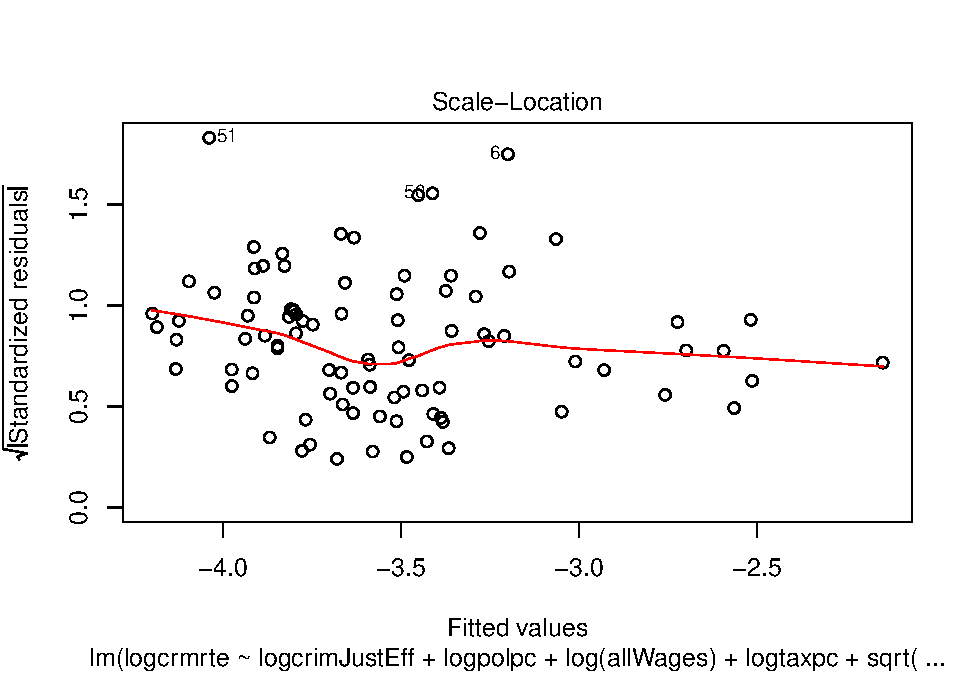
\includegraphics{Bagnard_Gaustad_Hartman_Leung_Lab_3_files/figure-latex/unnamed-chunk-91-3.pdf}
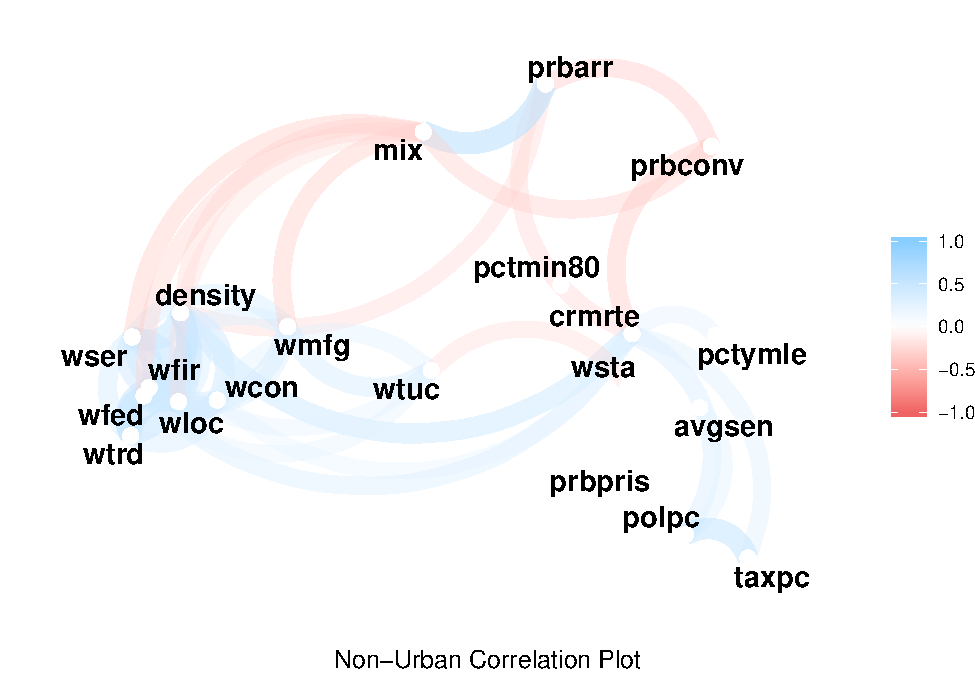
\includegraphics{Bagnard_Gaustad_Hartman_Leung_Lab_3_files/figure-latex/unnamed-chunk-91-4.pdf}

\textbf{Model 2 CLM Assumptions:} * \textbf{MLR1} Discussed above. *
\textbf{MLR2} Discussed above.

\begin{itemize}
\tightlist
\item
  \textbf{MLR3: Non-perfect Collinearity} We will use the VIF function
  to provide evidence that our variables in model2 are not perfectly
  multicollinear. As we can see from the VIF results, below, all of the
  variables' values are less than five, which allows us to conclude
  model2 is free from multicollinearity.
\end{itemize}

\begin{Shaded}
\begin{Highlighting}[]
\KeywordTok{vif}\NormalTok{(model2)}
\end{Highlighting}
\end{Shaded}

\begin{verbatim}
##        logcrimJustEff              logpolpc         log(allWages) 
##              1.401606              1.599426              2.004405 
##              logtaxpc sqrt(dfCrime$density) 
##              1.340363              2.385900
\end{verbatim}

\begin{itemize}
\tightlist
\item
  \textbf{MLR4: Zero Conditional Mean} The residual vs.~fitted chart,
  below, gives us evidence that we meet the zero conditional mean
  assumption as the majority of the residual means lie close to zero.
  The exceptions to this trend, lie on the right side of the chart where
  there are fewer data points (evidence for heteroscedasticity - see
  MLR5, below).
\end{itemize}

\begin{Shaded}
\begin{Highlighting}[]
\KeywordTok{plot}\NormalTok{(model2, }\DataTypeTok{which=}\DecValTok{1}\NormalTok{)}
\end{Highlighting}
\end{Shaded}

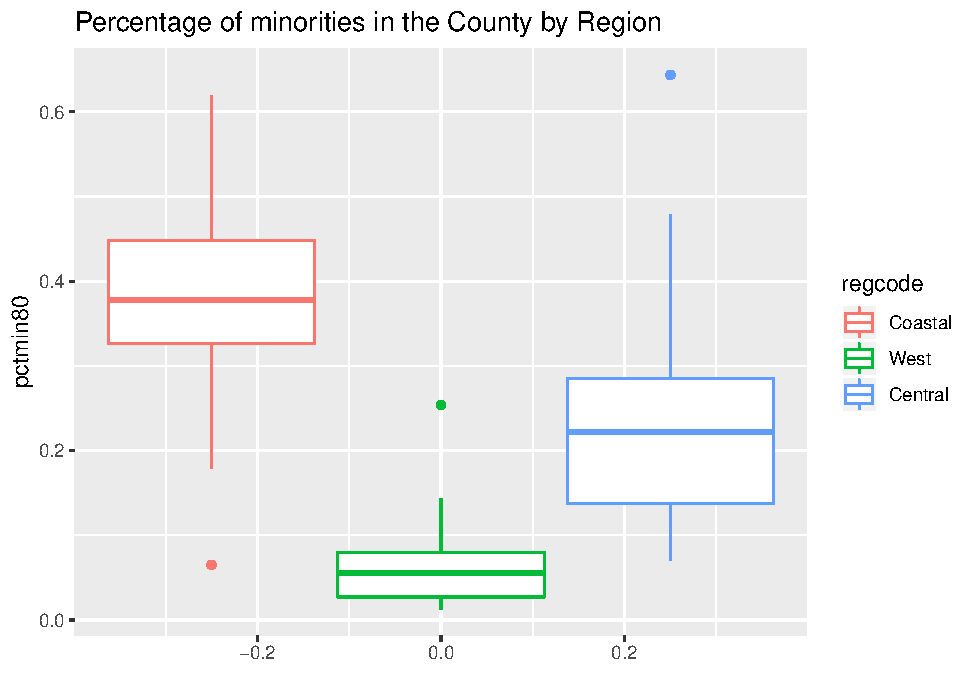
\includegraphics{Bagnard_Gaustad_Hartman_Leung_Lab_3_files/figure-latex/unnamed-chunk-93-1.pdf}

\begin{itemize}
\tightlist
\item
  \textbf{MLR5: Homoscedasticity} The above Residuals vs Fitted graph
  provides evidence of heteroscedasticity as right side of the chart
  have fewer datepoints. To provide further evidence of
  heteroscedasticity, we will use the White test with vcovHC
\end{itemize}

-- AXLB - WIP

\begin{Shaded}
\begin{Highlighting}[]
\KeywordTok{coeftest}\NormalTok{(model2, }\DataTypeTok{vcov=}\NormalTok{vcovHC)}
\end{Highlighting}
\end{Shaded}

\begin{verbatim}

t test of coefficients:

                      Estimate Std. Error t value Pr(>|t|)   
(Intercept)           -5.08471    5.39080 -0.9432 0.348274   
logcrimJustEff        -0.29992    0.13220 -2.2686 0.025854 * 
logpolpc               0.23648    0.23857  0.9912 0.324426   
log(allWages)          0.18618    0.61038  0.3050 0.761108   
logtaxpc               0.12275    0.24416  0.5028 0.616454   
sqrt(dfCrime$density)  0.47778    0.15108  3.1625 0.002177 **
---
Signif. codes:  0 '***' 0.001 '**' 0.01 '*' 0.05 '.' 0.1 ' ' 1
\end{verbatim}

\begin{itemize}
\tightlist
\item
  \textbf{MLR6: Normal Distribution of Errors} The Normal Q-Q plot,
  below, provides evidence that our residuals follow a normal
  distribution. While there are some data points on the left and right
  side of the graph that stray from the diagonal line, since our data
  set has over 30 datapoints, per the CLT, we can assume residuals have
  a normal distribution.
\end{itemize}

\begin{Shaded}
\begin{Highlighting}[]
\KeywordTok{plot}\NormalTok{(model2, }\DataTypeTok{which=}\DecValTok{2}\NormalTok{)}
\end{Highlighting}
\end{Shaded}

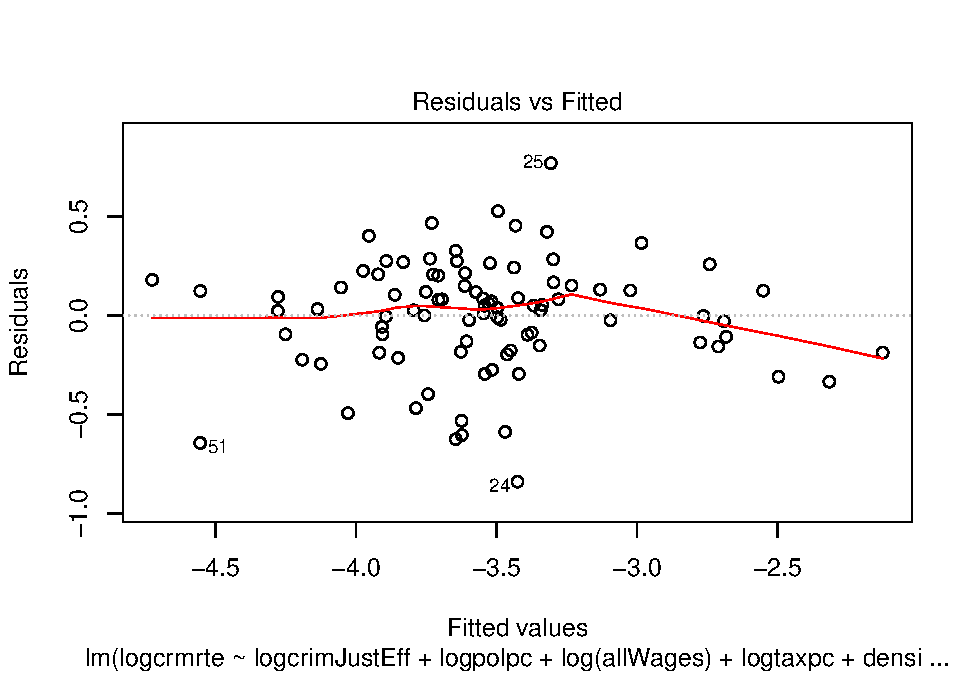
\includegraphics{Bagnard_Gaustad_Hartman_Leung_Lab_3_files/figure-latex/unnamed-chunk-95-1.pdf}

\begin{Shaded}
\begin{Highlighting}[]
\CommentTok{# hist(model2$residuals)}
\CommentTok{# shapiro.test(model2$residuals)}
\CommentTok{#null hypothesis: residuals drawn from population with a normal distribution. }
\CommentTok{#small p-value tells you if you can reject the null hypothesis. }
\CommentTok{#this test depends on sample size, it does not take very much deviation from normality for}
\CommentTok{#us to get a statistically significant result}
\end{Highlighting}
\end{Shaded}

\begin{Shaded}
\begin{Highlighting}[]
\KeywordTok{summary}\NormalTok{(model2)}
\end{Highlighting}
\end{Shaded}

\begin{verbatim}
## 
## Call:
## lm(formula = logcrmrte ~ logcrimJustEff + logpolpc + log(allWages) + 
##     logtaxpc + sqrt(dfCrime$density), data = dfCrime)
## 
## Residuals:
##      Min       1Q   Median       3Q      Max 
## -1.15778 -0.20916 -0.02745  0.28466  0.65767 
## 
## Coefficients:
##                       Estimate Std. Error t value Pr(>|t|)    
## (Intercept)            -5.0847     4.3863  -1.159 0.249647    
## logcrimJustEff         -0.2999     0.0815  -3.680 0.000411 ***
## logpolpc                0.2365     0.1518   1.558 0.122970    
## log(allWages)           0.1862     0.5124   0.363 0.717260    
## logtaxpc                0.1227     0.1705   0.720 0.473476    
## sqrt(dfCrime$density)   0.4778     0.1228   3.890 0.000200 ***
## ---
## Signif. codes:  0 '***' 0.001 '**' 0.01 '*' 0.05 '.' 0.1 ' ' 1
## 
## Residual standard error: 0.3681 on 84 degrees of freedom
## Multiple R-squared:  0.5752, Adjusted R-squared:  0.5499 
## F-statistic: 22.75 on 5 and 84 DF,  p-value: 2.313e-14
\end{verbatim}

The Adjusted R-squared variable penalizes for additional variables,
which means there is a chance that this value will decrease if the added
variables do not contribute to the model. By comparing the Adjusted
R-squared value between our first and second models, we see that
log(polpc), taxpc and density help describe log(crmrate). Our second
model has an Adjusted R-squared value of 0.5004, which means 50.04\% of
the variation in the \(log_{10}\) of crime rate is explained by the
explanatory variables used in this model. This is a significant increase
compared to our first model, that has an Adjusted R-squared value of
0.4520.

In addition, the F-statistic is 16.62 with a statistically significant
p-value of \textless{} 6.263e-11. As a result, we reject the null
hypothesis that none of the independent variables help to describe
log(crmrate).

Coefficient Analysis (assuming ceterus paribus): - logcrimJustEff:
-0.1607. This suggests that for a 1\% increase in criminal justice
efficiency, there is a 0.1607\% decrease in crime rate. - logpolpc:
0.3701. This suggests that for a 1\% increase in police per capita,
there is a 0.3701\% increase in crime rate. - allWages: 0.00006692. This
suggests that for a 1\% increase in total average weekly wage, there is
a 0.0067\% increase in crime rate. - taxpc: -0.001632. This suggests
that for a 1\% increase in tax per capita, there is a 0.1632\% decrease
in crime rate. - density: 0.06259. This suggests that for a 1\% increase
in density, there is a 6.259\% increase in crime rate.

\hypertarget{results---wip}{%
\subsubsection{\texorpdfstring{Results -
\textbf{WIP}}{Results - WIP}}\label{results---wip}}

\begin{itemize}
\tightlist
\item
  Standard Errors explanation will go here. Placeholder cell for now.
\end{itemize}

\hypertarget{conclusion-are-the-conclusions-they-draw-based-on-this-evaluation-appropriate-did-the-team-interpret-the-results-in-terms-of-their-research-question}{%
\subsubsection{Conclusion : Are the conclusions they draw based on this
evaluation appropriate? Did the team interpret the results in terms of
their research
question?}\label{conclusion-are-the-conclusions-they-draw-based-on-this-evaluation-appropriate-did-the-team-interpret-the-results-in-terms-of-their-research-question}}

Compared to model 1, the adjusted \(R^2\) of model 2 is only marginally
higher. This suggests that we should continue our analysis by focusing
on the join significance of the variables added in model 2.

\hypertarget{model-3}{%
\subsection{Model 3}\label{model-3}}

\hypertarget{introduction-3}{%
\subsubsection{Introduction}\label{introduction-3}}

Despite the improvements in the accuracy of model 2 over model 1, we are
still only explaining about 55\% of the variation in our data. As a
result, we propose to also analyse the topic of demographics which could
have an effect on both of our key explanatory variables.

One key component of demographics is the race of the county inhabitants
and how they are perceived and treated by others, especially for
minorities in the population. For example, systemic racism could have an
important effect on: * Criminal Justice Effectiveness: If police,
lawyers and judges are racially biased, this could lead to more arrests
and more convictions regardless of the strength of the legal case and
the evidence. As a result, we hypothesize the crime rate would increase.
* Economic Opportunity: Racism could prohibit members of the minority
from having access to education, jobs and higher wages. Racism could
also limit access to healthcare and social programmes which has a
negative effect on economic opportunity.

However, since we cannot directly measure racism, we have to
operationalize this covariate by examining its effect in the real world.
We propose to use the variable pctmin80, which represents the percentage
of minorities in the population of the county. This is a good indicator
that is also a linear parameter: given a higher the percentage of
minorities, we should expect to see a greater effect.

We propose to operationalize gender and age with the variable

We have also chosen not to include other variables from our dataset in
our model: * Region: While geographical indicators are also important,
particularly as they may represent clusters of jobs and skilled workers,
it is not a linear parameter (i.e.~we can not simply increase a region
by ``1'' and expect to see an effect on the crime rate.``) * Urban: We
believe the variable''density" better explains the same effects as
``urban'', while also being a linear parameter. In addition, there may
be data points that failed to meet the cutoff for being defined as
urban, but may still see the same effects as being urban and hence may
distort our analysis. * Age and Gender: While age and gender are
important demographic variables, the only variable in our dataset is
pctymle which provides the percentage of young males in the population.
However, given that this variable encompasses both male and young, we
may not be able to discern if age or gender has the larger effect (if
any at all).

\hypertarget{model-3-eda-and-data-transformations}{%
\subsubsection{Model 3 EDA and Data
Transformations}\label{model-3-eda-and-data-transformations}}

\textbf{Percentage Minority:} From the summary and boxplot below, we can
see that the percentage of minorities ranges from 0.0154 - 0.6435, with
a mean of 0.2621. We note that there are no major outliers.

In addition from the scatterplots below, we see that using applying log
on pctmin80 exposes a more linear relationship with the points more
balanced on either side of the trendline. As a result, we will use the
log-transformed version of pctmin80.

\begin{Shaded}
\begin{Highlighting}[]
\KeywordTok{summary}\NormalTok{(dfCrime}\OperatorTok{$}\NormalTok{pctmin80)}
\end{Highlighting}
\end{Shaded}

\begin{verbatim}
   Min. 1st Qu.  Median    Mean 3rd Qu.    Max. 
0.01284 0.10024 0.24852 0.25713 0.38183 0.64348 
\end{verbatim}

\begin{Shaded}
\begin{Highlighting}[]
\KeywordTok{boxplot}\NormalTok{(dfCrime}\OperatorTok{$}\NormalTok{pctmin80)}
\end{Highlighting}
\end{Shaded}

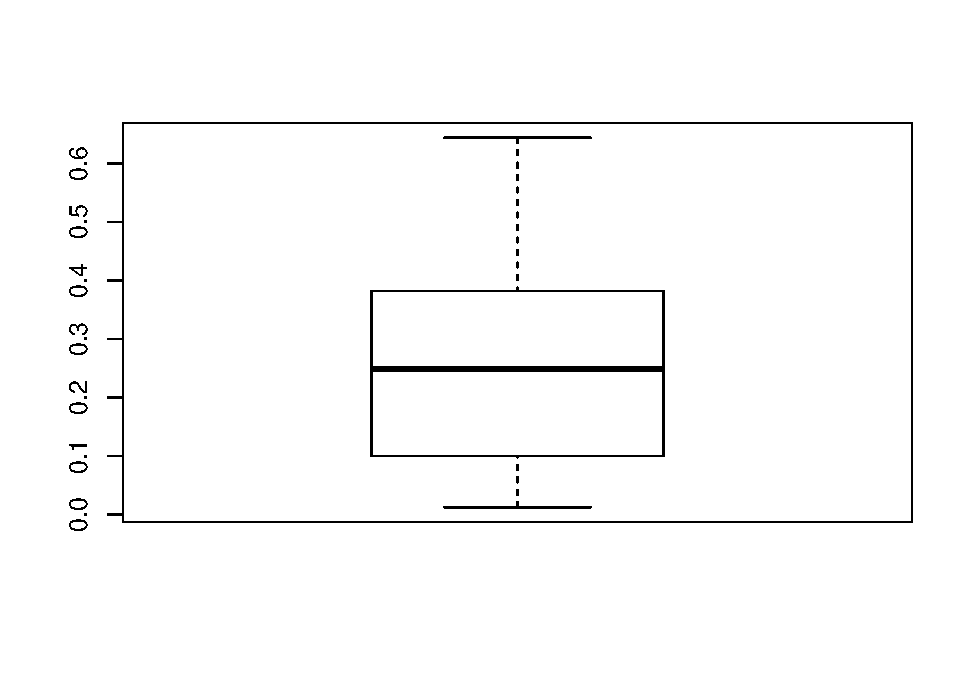
\includegraphics{Bagnard_Gaustad_Hartman_Leung_Lab_3_files/figure-latex/unnamed-chunk-97-1.pdf}

\begin{Shaded}
\begin{Highlighting}[]
\KeywordTok{plot}\NormalTok{(dfCrime}\OperatorTok{$}\NormalTok{pctmin80, dfCrime}\OperatorTok{$}\NormalTok{logcrmrte)}
\KeywordTok{abline}\NormalTok{(}\KeywordTok{lm}\NormalTok{(dfCrime}\OperatorTok{$}\NormalTok{logcrmrte}\OperatorTok{~}\NormalTok{dfCrime}\OperatorTok{$}\NormalTok{pctmin80))}
\end{Highlighting}
\end{Shaded}

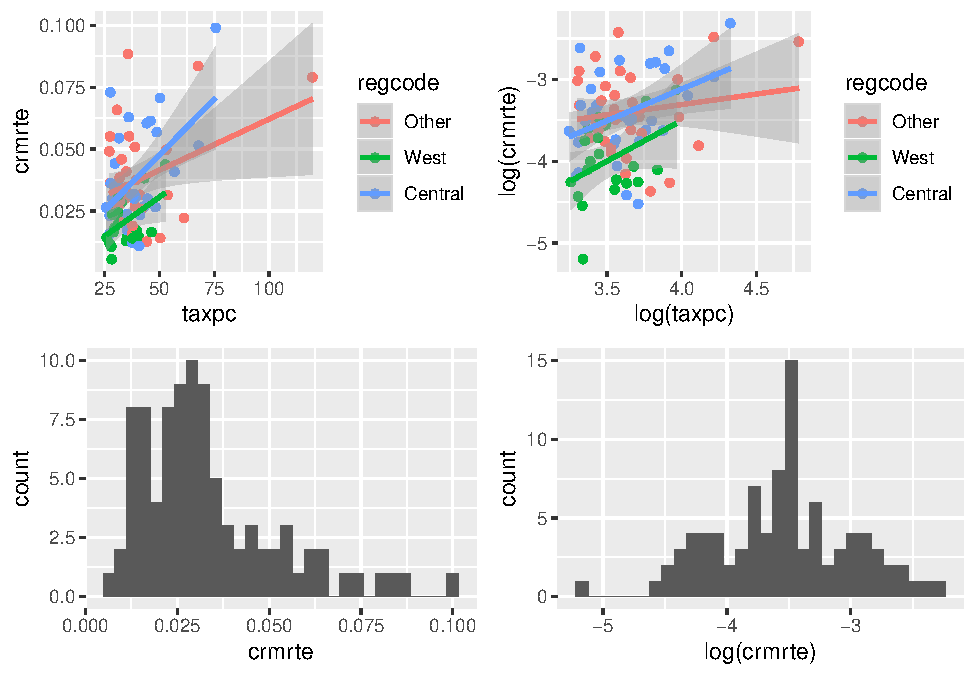
\includegraphics{Bagnard_Gaustad_Hartman_Leung_Lab_3_files/figure-latex/unnamed-chunk-98-1.pdf}

\begin{Shaded}
\begin{Highlighting}[]
\KeywordTok{plot}\NormalTok{(dfCrime}\OperatorTok{$}\NormalTok{logpctmin80, dfCrime}\OperatorTok{$}\NormalTok{logcrmrte)}
\KeywordTok{abline}\NormalTok{(}\KeywordTok{lm}\NormalTok{(dfCrime}\OperatorTok{$}\NormalTok{logcrmrte}\OperatorTok{~}\NormalTok{dfCrime}\OperatorTok{$}\NormalTok{logpctmin80))}
\end{Highlighting}
\end{Shaded}

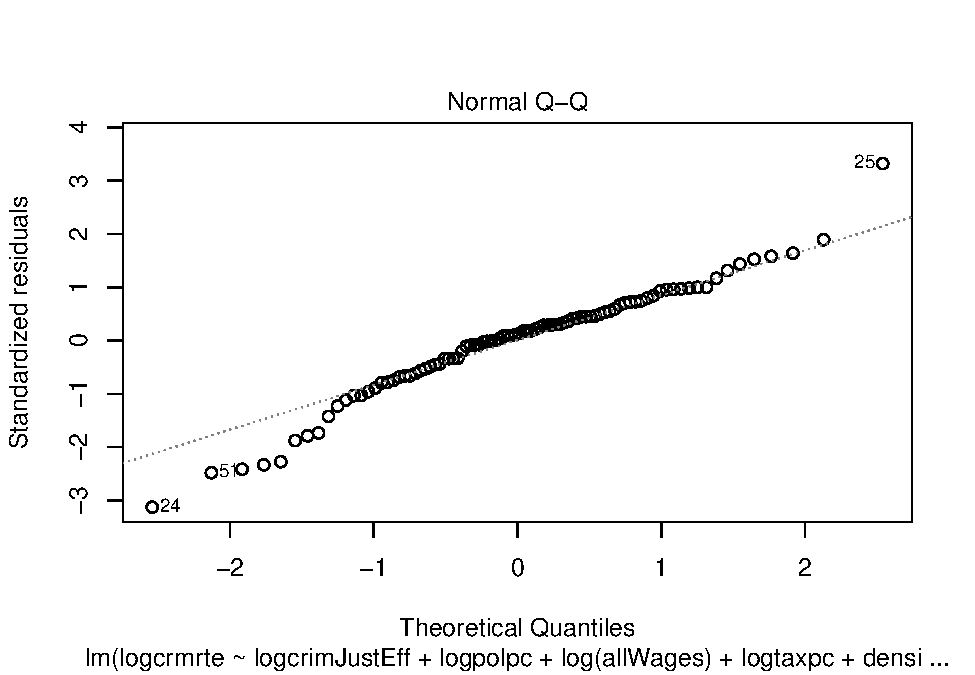
\includegraphics{Bagnard_Gaustad_Hartman_Leung_Lab_3_files/figure-latex/unnamed-chunk-98-2.pdf}

\hypertarget{model-3-linear-model}{%
\subsubsection{Model 3 Linear Model}\label{model-3-linear-model}}

\begin{Shaded}
\begin{Highlighting}[]
\CommentTok{## Testing}

\CommentTok{##dfCrime <- dfCrime[dfCrime$county != 55,]}
\CommentTok{##dfCrime <- dfCrime[dfCrime$county != 115,]}
\NormalTok{dfCrime}
\end{Highlighting}
\end{Shaded}

\begin{verbatim}
##    county year    crmrte    prbarr   prbconv  prbpris avgsen       polpc
## 1       1   87 0.0356036 0.2982700 0.5275960 0.436170   6.71 0.001827860
## 2       3   87 0.0152532 0.1320290 1.4814800 0.450000   6.35 0.000745880
## 3       5   87 0.0129603 0.4444440 0.2678570 0.600000   6.76 0.001234310
## 4       7   87 0.0267532 0.3647600 0.5254240 0.435484   7.14 0.001529940
## 5       9   87 0.0106232 0.5182190 0.4765630 0.442623   8.22 0.000860180
## 6      11   87 0.0146067 0.5246640 0.0683761 0.500000  13.00 0.002882030
## 7      13   87 0.0296409 0.3650040 0.5206070 0.420833  10.55 0.001337710
## 8      15   87 0.0202814 0.3921110 0.7692310 0.507692  10.64 0.001035250
## 9      17   87 0.0304289 0.2515990 0.4364410 0.436893   7.32 0.001297610
## 10     19   87 0.0221567 0.1628600 1.2256100 0.333333  10.34 0.002024250
## 11     21   87 0.0437355 0.2347600 0.3347010 0.429072  10.62 0.001829580
## 12     23   87 0.0269836 0.2891210 0.4037800 0.365957   7.07 0.001461110
## 13     25   87 0.0302542 0.3235480 0.4067800 0.492647   8.01 0.001971400
## 14     27   87 0.0382489 0.2680180 0.3529410 0.321429  11.69 0.001450130
## 15     33   87 0.0159189 0.2709500 0.5154640 0.480000   7.32 0.000755930
## 16     35   87 0.0408569 0.2660260 0.3253010 0.370370  10.06 0.001894440
## 17     37   87 0.0226017 0.3218670 0.3854960 0.316832   8.69 0.001305010
## 18     39   87 0.0119154 0.3083330 0.9729730 0.291667  11.58 0.001191540
## 19     41   87 0.0257713 0.3072460 0.4528300 0.520833  17.41 0.001493990
## 20     45   87 0.0362807 0.2026270 0.4505670 0.474820   8.96 0.001215310
## 21     47   87 0.0313623 0.1829270 0.7633330 0.270742   7.79 0.001281270
## 22     49   87 0.0374979 0.2644200 0.3718790 0.356890   8.70 0.001485320
## 23     51   87 0.0883849 0.1552480 0.2598330 0.407628  11.93 0.001908020
## 24     53   87 0.0140655 0.3031910 0.1403510 0.250000  11.96 0.001122250
## 25     55   87 0.0790163 0.2246280 0.2078310 0.304348  13.57 0.004009620
## 26     57   87 0.0300216 0.2220020 0.7369090 0.320624  10.47 0.001361910
## 27     59   87 0.0233327 0.2277530 0.6225170 0.425532   6.50 0.001196550
## 28     61   87 0.0233677 0.3981190 0.4934380 0.361702   8.77 0.001416220
## 29     63   87 0.0706599 0.1332250 0.4592160 0.363636  11.51 0.002376090
## 30     65   87 0.0658801 0.2873300 0.1544520 0.403922   9.84 0.001857390
## 31     67   87 0.0614177 0.2172150 0.2482760 0.488426  10.57 0.002177470
## 32     69   87 0.0173158 0.2835050 0.7393940 0.418033   9.10 0.001071080
## 33     71   87 0.0544061 0.2431190 0.2295900 0.379175  11.29 0.002070280
## 34     77   87 0.0441957 0.1908760 0.5283020 0.488095   9.60 0.002467110
## 35     79   87 0.0156759 0.4115380 0.3084110 0.454545   6.19 0.001024960
## 36     81   87 0.0604498 0.3002150 0.2037250 0.431020  14.42 0.002435620
## 37     83   87 0.0315752 0.4563940 0.4572100 0.410256   7.85 0.001385320
## 38     85   87 0.0490712 0.1461320 0.5490200 0.428571   8.78 0.001437300
## 39     87   87 0.0286781 0.2151080 0.5484950 0.341463  11.11 0.001691800
## 40     89   87 0.0283836 0.2966460 0.3869260 0.415525   5.51 0.001264470
## 41     91   87 0.0384263 0.3430740 0.5899050 0.454545   8.79 0.001621890
## 42     93   87 0.0362222 0.3389020 0.5739440 0.484663   5.45 0.001426410
## 43     97   87 0.0334506 0.3022310 0.5950780 0.409774   6.62 0.001526650
## 44     99   87 0.0171865 0.1538460 1.2343800 0.556962  14.75 0.001859120
## 45    101   87 0.0409403 0.1499360 0.5714290 0.473881   9.65 0.001400450
## 46    105   87 0.0514152 0.3814000 0.3842360 0.381410   8.81 0.001956140
## 47    107   87 0.0497552 0.2128950 0.3643530 0.450216   8.47 0.001687470
## 48    109   87 0.0230995 0.1627690 0.7816090 0.411765   9.12 0.001080430
## 49    111   87 0.0183048 0.2021120 0.5223880 0.542857  11.06 0.001187190
## 50    113   87 0.0142071 0.1798780 0.2203390 0.461538   6.39 0.001516000
## 51    115   87 0.0055332 0.3340234 1.0433771 0.500000  20.70 0.001948778
## 52    117   87 0.0268723 0.3704740 0.7932330 0.236967  11.83 0.001197650
## 53    119   87 0.0989659 0.1490940 0.3478000 0.486183   7.13 0.002231350
## 54    123   87 0.0300184 0.4874300 0.2263610 0.443038   6.49 0.001760860
## 55    125   87 0.0266287 0.2690430 0.4389610 0.396450   7.36 0.002009710
## 56    127   87 0.0291496 0.1796160 1.3581400 0.335616  15.99 0.001582890
## 57    129   87 0.0834982 0.2366010 0.3934130 0.415158   9.57 0.002558490
## 58    131   87 0.0189848 0.6890240 0.4955750 0.401786   9.97 0.001215490
## 59    133   87 0.0551287 0.2669600 0.2719470 0.334951   8.99 0.001544570
## 60    135   87 0.0628972 0.0927700 0.4777330 0.385593  11.92 0.002338710
## 61    137   87 0.0126662 0.2071430 1.0689700 0.322581   6.18 0.000814260
## 62    139   87 0.0243470 0.5226960 0.2894740 0.345455  14.22 0.001674480
## 63    141   87 0.0314610 0.2386360 0.4126980 0.487179  13.18 0.001271150
## 64    143   87 0.0265806 0.3178570 0.3146070 0.250000   9.36 0.000854380
## 65    145   87 0.0299856 0.3547330 0.3404910 0.594595   8.47 0.001370400
## 66    147   87 0.0551686 0.2215420 0.4267780 0.443137   7.73 0.002188740
## 67    149   87 0.0164987 0.2719670 1.0153800 0.227273  14.62 0.001518710
## 68    151   87 0.0264557 0.2991980 0.3601530 0.340426  12.57 0.001324300
## 69    153   87 0.0317563 0.3453680 0.5207100 0.458333  11.33 0.001384470
## 70    155   87 0.0312279 0.4082000 0.5598230 0.386544   8.71 0.001459250
## 71    157   87 0.0305908 0.2782870 0.4436810 0.377709   7.48 0.001917770
## 72    159   87 0.0362330 0.2435900 0.4929400 0.476563   8.64 0.001586190
## 73    161   87 0.0200070 0.4824250 0.5081970 0.451613   7.98 0.001248240
## 74    163   87 0.0215728 0.3109870 0.4011980 0.455224  11.25 0.001365870
## 75    165   87 0.0508341 0.3406790 0.4685310 0.432836   7.42 0.001513820
## 76    167   87 0.0238285 0.3622700 0.3225810 0.371429  10.48 0.001551440
## 77    169   87 0.0121033 0.3433870 0.7229730 0.448598  12.36 0.001095200
## 78    171   87 0.0243954 0.1756490 0.9090910 0.458333   8.67 0.001574420
## 79    173   87 0.0139937 0.5304350 0.3278690 0.150000   6.64 0.003163790
## 80    175   87 0.0164932 0.3503480 0.4105960 0.387097   7.31 0.001645490
## 81    179   87 0.0318720 0.3775430 0.3286640 0.426230   9.90 0.001478200
## 82    181   87 0.0729479 0.1825900 0.3430230 0.548023   7.06 0.001729480
## 83    183   87 0.0568423 0.2042160 0.3819080 0.367347  12.15 0.002127510
## 84    185   87 0.0108703 0.1952660 2.1212101 0.442857   5.38 0.001222100
## 85    187   87 0.0345231 0.3326690 0.4431140 0.432432   6.98 0.001169110
## 86    189   87 0.0313130 0.1613810 0.3005780 0.288462  12.27 0.002278370
## 87    191   87 0.0458895 0.1722570 0.4500000 0.421053   9.59 0.001227330
## 88    193   87 0.0235277 0.2660550 0.5888590 0.423423   5.86 0.001178870
## 90    195   87 0.0313973 0.2013970 1.6705199 0.470588  13.02 0.004459230
## 91    197   87 0.0141928 0.2075950 1.1829300 0.360825  12.23 0.001185730
##      density     taxpc west central urban  pctmin80     wcon     wtuc
## 1  2.4226327  30.99368    0       1     0 0.2021870 281.4259 408.7245
## 2  1.0463320  26.89208    0       1     0 0.0791632 255.1020 376.2542
## 3  0.4127659  34.81605    1       0     0 0.0316053 226.9470 372.2084
## 4  0.4915572  42.94759    0       1     0 0.4791610 375.2345 397.6901
## 5  0.5469484  28.05474    1       0     0 0.0179619 292.3077 377.3126
## 6  0.6113361  35.22974    1       0     0 0.0154070 250.4006 401.3378
## 7  0.5169492  30.69649    0       0     0 0.3217940 238.3064 366.3004
## 8  0.3009986  34.00304    0       0     0 0.6105400 253.5926 353.2182
## 9  0.3503982  34.96204    0       0     0 0.4038900 193.6432 346.6011
## 10 0.5767442  61.15251    0       0     0 0.2431170 260.1381 613.2261
## 11 2.6024280  52.62629    1       0     1 0.0962444 313.4738 433.8580
## 12 1.5119047  29.08280    1       0     0 0.0793198 284.9890 400.7398
## 13 2.5741758  33.03621    0       1     0 0.1509980 315.7290 384.6154
## 14 1.4989384  43.06339    1       0     0 0.0645795 292.7350 428.5023
## 15 0.5257009  27.38110    0       1     0 0.4391690 218.8868 286.4157
## 16 2.9242425  56.86211    0       1     0 0.1008380 346.5888 469.2220
## 17 0.5127119  34.70248    0       1     0 0.2780790 307.2780 462.4408
## 18 0.4623894  27.27564    1       0     0 0.0394549 277.5575 390.1895
## 19 0.7417582  41.76929    0       0     0 0.4264210 256.4102 379.0005
## 20 1.8440171  30.84900    0       1     0 0.2174990 318.3808 403.0558
## 21 0.5639659  32.66050    0       0     0 0.3340320 367.8286 342.5724
## 22 1.1440799  39.23048    0       0     0 0.2990720 292.8322 406.5041
## 23 3.9345510  35.69936    0       0     1 0.3777920 283.6695 412.4720
## 24 0.5351562  50.38139    0       0     0 0.1790960 266.4504 202.4292
## 25 0.5115089 119.76145    0       0     0 0.0649622 309.5238 445.2762
## 26 2.2518249  28.59199    0       1     0 0.1099570 324.6088 418.6380
## 27 1.0262172  41.07194    0       1     0 0.1087040 280.8989 335.4590
## 28 0.5079365  32.59961    0       0     0 0.3499950 244.2002 308.5150
## 29 5.6744967  50.19918    0       1     1 0.3822300 349.3267 548.9865
## 30 1.1679842  30.62824    0       0     0 0.5169320 362.1527 540.1061
## 31 6.4271846  45.89987    0       1     1 0.2565460 206.5527 379.5547
## 32 0.7125506  35.37642    0       1     0 0.4232240 372.1622 508.2035
## 33 4.8347340  31.53658    0       1     1 0.1331500 291.4508 595.3719
## 34 0.7172285  29.70588    0       1     0 0.4545130 254.7925 391.7379
## 35 0.6203008  37.50189    0       0     0 0.4546750 223.9199 320.5128
## 36 5.1244240  44.21059    0       1     1 0.2639410 404.8150 489.3144
## 37 0.7817680  41.08650    0       0     0 0.5056250 269.1710 480.7692
## 38 1.0815308  27.16143    0       0     0 0.2562870 245.8896 448.7180
## 39 0.8648649  32.82694    1       0     0 0.0269921 250.7271 437.9284
## 40 1.8155080  32.48096    1       0     0 0.0431205 293.8034 501.9174
## 41 0.6713483  31.85298    0       0     0 0.5680850 289.2227 431.9210
## 42 0.6112532  27.47967    0       0     0 0.5808270 231.1391 187.6173
## 43 1.5662020  29.97040    0       1     0 0.1840120 333.0927 421.6986
## 44 0.5478615  39.57348    1       0     0 0.1428460 259.7841 417.2099
## 45 0.9962264  34.87021    0       0     0 0.2094790 245.6298 378.1590
## 46 1.5984555  67.84798    0       1     0 0.2354980 314.0595 401.1326
## 47 1.5024875  53.17796    0       0     0 0.3904780 279.4214 350.1326
## 48 1.5939597  27.32160    0       1     0 0.0968564 270.0951 374.0296
## 49 0.8306636  29.58239    1       0     0 0.0552725 245.1514 571.5438
## 50 0.4487427  40.80142    1       0     0 0.0239865 244.7552 412.0879
## 51 0.3858093  28.19310    1       0     0 0.0128365 204.2206 503.2351
## 52 0.5813449  38.81493    0       0     0 0.4542550 242.3077 424.7286
## 53 8.8276520  75.67243    0       1     1 0.2854600 436.7666 548.3239
## 54 0.4938776  38.45734    0       1     0 0.2596020 345.1677 396.2704
## 55 0.8202568  48.15414    0       1     0 0.2258190 261.5648 457.5350
## 56 1.3388889  32.02376    0       0     0 0.3427990 290.9091 426.3901
## 57 6.2864866  67.67963    0       0     1 0.2304410 315.5760 392.0999
## 58 0.4126394  37.70006    0       0     0 0.6194210 225.8647 375.2345
## 59 1.6500655  27.46926    0       0     0 0.2638140 264.0406 318.9644
## 60 2.1575000  35.99248    0       1     0 0.1952630 316.0858 420.8830
## 61 0.3167155  44.29367    0       0     0 0.3304480 299.4956 356.1254
## 62 1.3333334  29.49915    0       0     0 0.3806130 278.0824 441.5954
## 63 0.3005714  35.97390    0       0     0 0.3985150 257.9737 388.3136
## 64 0.4349594  31.22779    0       0     0 0.3863590 250.8361 373.9316
## 65 0.7788945  44.64758    0       1     0 0.3295160 305.3435 538.8488
## 66 1.5159818  36.18621    0       0     0 0.3564110 295.1822 379.8962
## 67 0.6092437  29.03402    1       0     0 0.1000460 223.6136 437.0629
## 68 1.2737643  25.69287    0       1     0 0.0697606 340.4792 415.1317
## 69 0.9622641  37.22833    0       1     0 0.2852840 262.6642 294.6650
## 70 1.1296101  31.37446    0       0     0 0.6144970 253.2447 407.0929
## 71 1.5096661  39.16965    0       1     0 0.2160360 317.5345 409.7771
## 72 2.0192678  27.76489    0       1     0 0.1699130 334.1035 475.3228
## 73 1.0052817  31.34530    1       0     0 0.1303660 275.4970 402.5045
## 74 0.5353749  34.01291    0       0     0 0.3634950 217.1781 415.2824
## 75 1.0783699  38.74739    0       0     0 0.4242560 309.1764 471.3424
## 76 1.2752526  35.09686    0       1     0 0.1257910 293.5538 419.0362
## 77 0.8008850  37.70785    0       1     0 0.0767092 345.6391 588.6970
## 78 1.1521336  31.15306    1       0     0 0.0564349 385.3424 412.5212
## 79 0.5005005  37.72702    1       0     0 0.2539140 231.6960 213.6752
## 80 0.6878307  46.41461    1       0     0 0.0603408 253.3395 402.5045
## 81 1.2816901  38.44067    0       1     0 0.1788580 314.4250 361.1018
## 82 1.5702811  27.59179    0       1     0 0.4462830 244.8362 365.4716
## 83 4.3887587  48.76492    0       1     1 0.2344360 360.9549 528.5593
## 84 0.3887588  40.82454    0       1     0 0.6434820 226.8245 331.5650
## 85 0.4427711  34.71814    0       0     0 0.4421320 264.4231 421.3483
## 86 1.1019108  31.33022    1       0     0 0.0198320 238.3758 354.2510
## 87 1.7725632  32.74533    0       0     0 0.3442830 318.0599 400.8570
## 88 0.8138298  28.51783    1       0     0 0.0593109 285.8289 480.1948
## 90 1.7459893  53.66693    0       0     0 0.3743110 315.1641 377.9356
## 91 0.8898810  25.95258    1       0     0 0.0546081 314.1660 341.8803
##        wtrd     wfir     wser   wmfg   wfed   wsta   wloc        mix
## 1  221.2701 453.1722 274.1775 334.54 477.58 292.09 311.91 0.08016878
## 2  196.0101 258.5650 192.3077 300.38 409.83 362.96 301.47 0.03022670
## 3  229.3209 305.9441 209.6972 237.65 358.98 331.53 281.37 0.46511629
## 4  191.1720 281.0651 256.7214 281.80 412.15 328.27 299.03 0.27362204
## 5  206.8215 289.3125 215.1933 290.89 377.35 367.23 342.82 0.06008584
## 6  187.8255 258.5650 237.1507 258.60 391.48 325.71 275.22 0.31952664
## 7  205.5358 310.1737 259.3391 303.42 449.84 350.72 283.76 0.15237226
## 8  199.2377 356.1254 206.2816 235.05 416.49 370.62 297.13 0.23495702
## 9  202.9595 268.3363 208.2520 339.76 389.51 322.06 278.39 0.21818182
## 10 191.2452 290.5141 266.0934 567.06 403.15 258.33 299.44 0.05334728
## 11 228.1740 363.7671 318.3635 378.90 496.13 381.30 335.36 0.06289308
## 12 213.1840 325.0271 315.0242 327.45 463.67 361.21 308.32 0.08400646
## 13 220.5897 358.6328 318.0335 355.59 486.36 411.08 357.44 0.08848315
## 14 213.4620 316.9436 292.3517 309.27 450.28 283.60 310.85 0.08957055
## 15 195.1995 368.2488 172.4733 324.45 357.16 407.54 268.44 0.15112540
## 16 277.2925 359.3117 296.8491 341.32 525.51 360.68 333.32 0.18122160
## 17 227.7858 305.6546 231.3615 321.90 460.62 393.29 321.53 0.08100930
## 18 180.0634 295.8580 246.0152 270.78 397.33 313.06 239.17 0.13744076
## 19 238.5589 271.7391 232.5916 332.07 451.84 389.99 312.05 0.09872611
## 20 248.7759 301.8632 293.1148 367.42 463.37 352.35 320.82 0.08594864
## 21 194.6777 352.6135 256.4102 355.83 426.56 313.71 313.84 0.12405757
## 22 212.4851 312.6954 304.3066 375.32 474.30 297.69 290.48 0.10692308
## 23 213.7524 324.8357 257.3344 441.72 433.94 367.34 333.71 0.10474319
## 24 219.7802 305.9441 223.8502 250.42 371.79 383.72 296.64 0.08045977
## 25 189.7436 284.5933 221.3903 319.21 338.91 361.68 326.08 0.08437271
## 26 225.5296 338.5699 261.3512 324.67 496.07 325.15 314.01 0.07497714
## 27 210.3365 317.3077 316.6645 316.57 428.33 388.92 307.25 0.11616162
## 28 214.2203 327.1213 203.8864 266.58 414.84 333.46 308.05 0.16707317
## 29 238.9154 435.1107 391.3081 646.85 563.77 415.51 362.58 0.07585382
## 30 209.0579 316.2955 216.4589 313.71 543.03 348.88 329.16 0.09364294
## 31 189.1807 278.0352 230.4981 275.72 419.07 400.59 313.55 0.21999694
## 32 266.7794 466.0016 347.6609 560.78 516.05 381.03 388.09 0.07977737
## 33 240.3673 348.0254 295.2301 358.95 509.43 359.11 339.58 0.10186080
## 34 197.6995 311.3553 199.4458 360.21 512.30 369.75 329.34 0.17905165
## 35 171.0329 334.4482 250.0000 218.30 353.31 385.19 323.08 0.28078818
## 36 308.5762 420.8864 305.1543 448.86 563.72 426.47 333.64 0.10255422
## 37 200.3768 297.2437 239.2233 360.27 466.61 367.24 302.63 0.09106830
## 38 198.6254 248.1390 264.6729 310.86 437.03 397.54 327.37 0.14886613
## 39 196.5065 288.4615 243.4706 588.99 488.76 346.32 294.21 0.09794629
## 40 214.2170 334.1840 258.3238 443.70 496.28 308.01 305.71 0.09090909
## 41 198.0064 253.3395 266.4674 316.19 430.64 314.75 297.34 0.09869203
## 42 161.3771 254.5249 182.0196 298.78 471.09 400.11 292.98 0.18528996
## 43 222.9622 338.7534 282.9701 346.51 480.14 351.17 330.93 0.08431085
## 44 168.2692 301.5734 247.6291 258.99 442.76 387.02 291.44 0.01960784
## 45 203.1547 307.2585 232.1825 325.03 459.90 350.27 317.12 0.09447166
## 46 237.8523 323.9486 274.8686 352.08 463.11 267.78 343.13 0.10368066
## 47 202.9344 333.9183 276.2629 350.63 496.75 332.12 324.97 0.11912815
## 48 226.4881 335.4204 230.3086 320.20 453.61 389.34 302.93 0.05424063
## 49 179.5039 327.9666 251.4270 260.35 384.15 354.41 304.91 0.06763285
## 50 154.2090 256.4102 265.1301 291.10 337.09 374.11 246.65 0.05128205
## 51 217.4908 342.4658 245.2061 448.42 442.20 340.39 386.12 0.10000000
## 52 167.0511 282.4099 229.0151 327.29 383.88 360.66 302.03 0.07485030
## 53 354.6761 509.4655 354.3007 494.30 568.40 329.22 379.77 0.16869897
## 54 193.0723 272.2941 242.4605 277.34 345.09 328.00 325.77 0.31135532
## 55 199.5847 299.7388 320.1325 277.68 447.87 361.24 300.77 0.07110778
## 56 257.6008 441.1413 305.7612 329.87 508.61 380.30 329.71 0.06305506
## 57 220.4530 363.2880 292.7027 464.49 548.49 421.36 319.08 0.07871422
## 58 220.9747 307.6923 172.6281 278.70 432.81 370.81 259.78 0.16725978
## 59 183.2609 265.1232 230.6581 258.25 326.10 329.43 301.64 0.12176319
## 60 179.1289 389.8522 292.2253 388.75 509.95 499.59 333.05 0.05091770
## 61 170.8711 170.9402 250.8361 192.96 360.84 283.90 321.73 0.06870229
## 62 201.3569 302.6724 260.5459 264.25 452.59 348.05 285.47 0.34879407
## 63 179.7050 263.7363 196.1453 255.56 374.78 380.29 294.98 0.20000000
## 64 178.3723 234.5216 133.0431 157.41 380.97 388.43 253.66 0.21212120
## 65 200.7432 302.1978 219.6343 334.65 414.63 298.78 295.00 0.22533333
## 66 205.4827 377.6978 274.6765 390.01 543.21 464.63 330.78 0.09345226
## 67 188.7683 353.2182 210.4415 289.43 421.34 342.92 301.23 0.11682243
## 68 218.7198 322.4150 278.1124 294.37 474.26 298.66 294.72 0.07342084
## 69 192.8994 267.3797 237.1590 301.29 467.08 350.24 302.25 0.16323297
## 70 200.2213 337.9095 262.9849 278.82 441.49 381.46 304.73 0.12516960
## 71 192.4181 302.6162 245.7938 418.48 478.48 342.13 318.07 0.12467756
## 72 260.2710 329.5464 265.4315 374.41 491.16 346.81 351.74 0.09146758
## 73 201.5675 279.2492 251.4202 334.92 450.28 277.60 302.83 0.11024390
## 74 196.5514 279.0347 238.6300 295.07 429.27 318.02 299.92 0.12108560
## 75 203.0162 294.4124 267.6852 374.25 442.38 381.14 285.50 0.09595300
## 76 221.0995 326.8283 253.0096 351.09 463.69 312.53 311.47 0.10925926
## 77 190.5555 331.5650 206.6858 306.42 406.62 348.37 306.68 0.13720317
## 78 224.7224 339.9547 253.6207 288.32 452.53 341.77 324.06 0.08207343
## 79 175.1604 267.0940 204.3792 193.01 334.44 414.68 304.32 0.41975310
## 80 172.6453 317.3394 257.8734 627.02 344.06 357.69 298.33 0.10230179
## 81 241.0034 342.6819 270.4866 349.63 459.32 387.16 376.45 0.13481072
## 82 279.2273 325.0271 213.5822 290.69 453.53 317.23 286.45 0.10003893
## 83 306.0835 430.0697 348.2754 444.45 597.95 453.08 362.99 0.08527010
## 84 167.3726 264.4231 251.5703 247.72 381.33 367.25 300.13 0.04968944
## 85 170.5293 282.0513 183.1502 297.14 390.94 356.91 267.08 0.29048842
## 86 180.9359 369.4332 253.2281 304.72 427.84 451.79 297.19 0.05719921
## 87 230.9888 320.0345 238.4958 295.26 334.55 375.45 327.62 0.08616445
## 88 268.3836 365.0196 295.9352 295.63 468.26 337.88 348.74 0.11050157
## 90 246.0614 411.4330 296.8684 392.27 480.79 303.11 337.28 0.15612382
## 91 182.8020 348.1432 212.8205 322.92 391.72 385.65 306.85 0.06756757
##       pctymle region regcode other nonurban   metro  logwcon  logwtuc
## 1  0.07787097      2       C     0        1 Outside 5.639869 6.013041
## 2  0.08260694      2       C     0        1 Outside 5.541664 5.930265
## 3  0.07211538      1       W     0        1 Outside 5.424716 5.919454
## 4  0.07353726      2       C     0        1 Outside 5.927551 5.985673
## 5  0.07069755      1       W     0        1 Outside 5.677807 5.933074
## 6  0.09891920      1       W     0        1 Outside 5.523062 5.994803
## 7  0.07073344      0       O     1        1 Outside 5.473557 5.903454
## 8  0.07430546      0       O     1        1 Outside 5.535729 5.867086
## 9  0.07769163      0       O     1        1 Outside 5.266017 5.848174
## 10 0.07713232      0       O     1        1 Outside 5.561213 6.418734
## 11 0.07219726      1       W     0        0  Inside 5.747716 6.072717
## 12 0.08397806      1       W     0        1 Outside 5.652451 5.993312
## 13 0.07641540      2       C     0        1 Outside 5.754884 5.952244
## 14 0.08353864      1       W     0        1 Outside 5.679268 6.060296
## 15 0.08005202      2       C     0        1 Outside 5.388555 5.657444
## 16 0.07891140      2       C     0        1 Outside 5.848139 6.151076
## 17 0.07154077      2       C     0        1 Outside 5.727753 6.136519
## 18 0.06973287      1       W     0        1 Outside 5.626028 5.966633
## 19 0.06355526      0       O     1        1 Outside 5.546779 5.937538
## 20 0.08013537      2       C     0        1 Outside 5.763248 5.999075
## 21 0.07381025      0       O     1        1 Outside 5.907617 5.836483
## 22 0.12224479      0       O     1        1 Outside 5.679600 6.007594
## 23 0.14223780      0       O     1        0  Inside 5.647810 6.022168
## 24 0.08476309      0       O     1        1 Outside 5.585188 5.310390
## 25 0.07613807      0       O     1        1 Outside 5.735035 6.098695
## 26 0.07873024      2       C     0        1 Outside 5.782621 6.037007
## 27 0.07756928      2       C     0        1 Outside 5.637995 5.815500
## 28 0.07579902      0       O     1        1 Outside 5.497989 5.731771
## 29 0.09468981      2       C     0        0  Inside 5.856007 6.308074
## 30 0.07622346      0       O     1        1 Outside 5.892066 6.291766
## 31 0.07647973      2       C     0        0  Inside 5.330556 5.938999
## 32 0.08181948      2       C     0        1 Outside 5.919330 6.230882
## 33 0.07939028      2       C     0        0  Inside 5.674871 6.389186
## 34 0.08345764      2       C     0        1 Outside 5.540450 5.970593
## 35 0.08120255      0       O     1        1 Outside 5.411288 5.769922
## 36 0.08310476      2       C     0        0  Inside 6.003430 6.193005
## 37 0.07521905      0       O     1        1 Outside 5.595347 6.175387
## 38 0.10694169      0       O     1        1 Outside 5.504883 6.106395
## 39 0.07600891      1       W     0        1 Outside 5.524365 6.082055
## 40 0.06795343      1       W     0        1 Outside 5.682911 6.218436
## 41 0.08729226      0       O     1        1 Outside 5.667197 6.068243
## 42 0.08633697      0       O     1        1 Outside 5.443019 5.234404
## 43 0.07655433      2       C     0        1 Outside 5.808421 6.044291
## 44 0.12894706      1       W     0        1 Outside 5.559851 6.033589
## 45 0.07609449      0       O     1        1 Outside 5.503826 5.935315
## 46 0.07365920      2       C     0        1 Outside 5.749583 5.994292
## 47 0.07455523      0       O     1        1 Outside 5.632721 5.858312
## 48 0.08050946      2       C     0        1 Outside 5.598774 5.924335
## 49 0.06861899      1       W     0        1 Outside 5.501876 6.348341
## 50 0.09171820      1       W     0        1 Outside 5.500259 6.021237
## 51 0.07253495      1       W     0        1 Outside 5.319201 6.221057
## 52 0.07632116      0       O     1        1 Outside 5.490208 6.051450
## 53 0.07916495      2       C     0        0  Inside 6.079399 6.306866
## 54 0.08119376      2       C     0        1 Outside 5.844030 5.982097
## 55 0.07415335      2       C     0        1 Outside 5.566682 6.125853
## 56 0.07400288      0       O     1        1 Outside 5.673011 6.055355
## 57 0.08109921      0       O     1        0  Inside 5.754400 5.971517
## 58 0.08356434      0       O     1        1 Outside 5.419936 5.927551
## 59 0.24871162      0       O     1        1 Outside 5.576103 5.765080
## 60 0.13302912      2       C     0        1 Outside 5.756014 6.042355
## 61 0.07098370      0       O     1        1 Outside 5.702100 5.875283
## 62 0.09625563      0       O     1        1 Outside 5.627917 6.090394
## 63 0.07572646      0       O     1        1 Outside 5.552858 5.961813
## 64 0.06769374      0       O     1        1 Outside 5.524800 5.924073
## 65 0.07275662      2       C     0        1 Outside 5.721437 6.289435
## 66 0.11421655      0       O     1        1 Outside 5.687593 5.939898
## 67 0.06215772      1       W     0        1 Outside 5.409920 6.080077
## 68 0.07763254      2       C     0        1 Outside 5.830354 6.028596
## 69 0.07570874      2       C     0        1 Outside 5.570876 5.685839
## 70 0.08183564      0       O     1        1 Outside 5.534356 6.009041
## 71 0.07771273      2       C     0        1 Outside 5.760587 6.015613
## 72 0.07705218      2       C     0        1 Outside 5.811451 6.163994
## 73 0.07362188      1       W     0        1 Outside 5.618577 5.997706
## 74 0.07472797      0       O     1        1 Outside 5.380718 6.028959
## 75 0.08548180      0       O     1        1 Outside 5.733912 6.155585
## 76 0.07687439      2       C     0        1 Outside 5.682061 6.037957
## 77 0.08280677      2       C     0        1 Outside 5.845395 6.377912
## 78 0.07735254      1       W     0        1 Outside 5.954132 6.022288
## 79 0.07462687      1       W     0        1 Outside 5.445426 5.364457
## 80 0.08436658      1       W     0        1 Outside 5.534730 5.997706
## 81 0.08703093      2       C     0        1 Outside 5.750746 5.889160
## 82 0.07977433      2       C     0        1 Outside 5.500589 5.901189
## 83 0.09935585      2       C     0        0  Inside 5.888753 6.270155
## 84 0.07008217      2       C     0        1 Outside 5.424176 5.803824
## 85 0.07794872      0       O     1        1 Outside 5.577550 6.043460
## 86 0.15092644      1       W     0        1 Outside 5.473849 5.870006
## 87 0.08828809      0       O     1        1 Outside 5.762240 5.993605
## 88 0.07819394      1       W     0        1 Outside 5.655393 6.174192
## 90 0.07945071      0       O     1        1 Outside 5.753093 5.934724
## 91 0.07419893      1       W     0        1 Outside 5.749922 5.834461
##     logwtrd  logwfir  logwser  logwmfg  logwfed  logwsta  logwloc
## 1  5.399384 6.116272 5.613776 5.812756 6.168732 5.677062 5.742715
## 2  5.278166 5.555147 5.259097 5.705048 6.015742 5.894293 5.708671
## 3  5.435122 5.723402 5.345665 5.470799 5.883267 5.803718 5.639671
## 4  5.253174 5.638586 5.547992 5.641198 6.021387 5.793836 5.700544
## 5  5.331856 5.667507 5.371537 5.672945 5.933173 5.905988 5.837206
## 6  5.235513 5.555147 5.468696 5.555282 5.969934 5.786007 5.617571
## 7  5.325620 5.737132 5.558136 5.715118 6.108892 5.859988 5.648129
## 8  5.294499 5.875283 5.329242 5.459798 6.031862 5.915177 5.694170
## 9  5.313006 5.592241 5.338749 5.828240 5.964890 5.774738 5.629023
## 10 5.253556 5.671652 5.583847 6.340465 5.999309 5.554238 5.701914
## 11 5.430109 5.896514 5.763194 5.937272 6.206838 5.943586 5.815205
## 12 5.362156 5.783909 5.752650 5.791335 6.139173 5.889459 5.731138
## 13 5.396305 5.882299 5.762157 5.873778 6.186949 6.018788 5.878968
## 14 5.363459 5.758724 5.677958 5.734215 6.109870 5.647565 5.739311
## 15 5.274022 5.908759 5.150242 5.782131 5.878184 6.010139 5.592627
## 16 5.625073 5.884190 5.693224 5.832820 6.264369 5.887991 5.809103
## 17 5.428406 5.722456 5.443981 5.774241 6.132573 5.974547 5.773091
## 18 5.193309 5.689880 5.505393 5.601307 5.984767 5.746395 5.477175
## 19 5.474616 5.604843 5.449284 5.805346 6.113328 5.966121 5.743163
## 20 5.516552 5.709974 5.680564 5.906506 6.138526 5.864625 5.770880
## 21 5.271345 5.865373 5.546779 5.874453 6.055753 5.748469 5.748883
## 22 5.358872 5.745230 5.718036 5.927779 6.161840 5.696053 5.671535
## 23 5.364818 5.783320 5.550377 6.090676 6.072906 5.906288 5.810272
## 24 5.392628 5.723402 5.410977 5.523140 5.918329 5.949913 5.692519
## 25 5.245674 5.651061 5.399927 5.765849 5.825735 5.890760 5.787143
## 26 5.418451 5.824731 5.565865 5.782809 6.206717 5.784287 5.749425
## 27 5.348709 5.759872 5.757843 5.757544 6.059894 5.963374 5.727662
## 28 5.367005 5.790331 5.317563 5.585674 6.027893 5.809523 5.730262
## 29 5.476110 6.075601 5.969495 6.472114 6.334646 6.029507 5.893245
## 30 5.342611 5.756677 5.377401 5.748469 6.297165 5.854728 5.796544
## 31 5.242703 5.627748 5.440242 5.619386 6.038038 5.992938 5.747959
## 32 5.586422 6.144189 5.851228 6.329329 6.246204 5.942878 5.961237
## 33 5.482168 5.852275 5.687755 5.883183 6.233292 5.883629 5.827710
## 34 5.286748 5.740935 5.295542 5.886687 6.238910 5.912827 5.797091
## 35 5.141856 5.812482 5.521461 5.385870 5.867346 5.953737 5.777900
## 36 5.731969 6.042363 5.720817 6.106711 6.334558 6.055542 5.810063
## 37 5.300200 5.694552 5.477398 5.886854 6.145494 5.906016 5.712511
## 38 5.291421 5.513989 5.578495 5.739343 6.080002 5.985296 5.791091
## 39 5.280696 5.664562 5.494996 6.378409 6.191872 5.847363 5.684294
## 40 5.366989 5.811692 5.554214 6.095149 6.207140 5.730132 5.722637
## 41 5.288299 5.534730 5.585252 5.756343 6.065273 5.751779 5.694876
## 42 5.083744 5.539399 5.204114 5.699708 6.155049 5.991739 5.680104
## 43 5.407002 5.825272 5.645341 5.847912 6.174078 5.861270 5.801907
## 44 5.125565 5.709014 5.511932 5.556789 6.093028 5.958476 5.674834
## 45 5.313968 5.727690 5.447524 5.783917 6.131009 5.858704 5.759280
## 46 5.471650 5.780585 5.616293 5.863858 6.137965 5.590166 5.838109
## 47 5.312883 5.810896 5.621353 5.859732 6.208087 5.805496 5.783733
## 48 5.422692 5.815385 5.439420 5.768946 6.117238 5.964453 5.713502
## 49 5.190197 5.792912 5.527153 5.562027 5.951033 5.870454 5.720017
## 50 5.038309 5.546779 5.580221 5.673667 5.820350 5.924550 5.507970
## 51 5.382157 5.836172 5.502099 6.105730 6.091762 5.830092 5.956148
## 52 5.118300 5.643360 5.433788 5.790847 5.950330 5.887936 5.710526
## 53 5.871205 6.233362 5.870146 6.203143 6.342825 5.796726 5.939566
## 54 5.263065 5.606883 5.490839 5.625244 5.843805 5.793014 5.786192
## 55 5.296238 5.702912 5.768735 5.626469 6.104503 5.889543 5.706346
## 56 5.551411 6.089365 5.722804 5.798699 6.231681 5.940960 5.798213
## 57 5.395684 5.895196 5.679158 6.140940 6.307169 6.043488 5.765442
## 58 5.398048 5.729100 5.151140 5.630136 6.070299 5.915690 5.559835
## 59 5.210911 5.580195 5.440936 5.553928 5.787204 5.797364 5.709234
## 60 5.188106 5.965768 5.677525 5.962936 6.234313 6.213788 5.808293
## 61 5.140910 5.141314 5.524800 5.262483 5.888435 5.648622 5.773713
## 62 5.305079 5.712651 5.562779 5.576896 6.114987 5.852346 5.654137
## 63 5.191317 5.574950 5.278856 5.543457 5.926339 5.940934 5.686908
## 64 5.183873 5.457548 4.890673 5.058854 5.942721 5.962113 5.535995
## 65 5.302026 5.711082 5.391964 5.813085 6.027387 5.699708 5.686975
## 66 5.325362 5.934095 5.615594 5.966172 6.297496 6.141241 5.801453
## 67 5.240520 5.867086 5.349208 5.667913 6.043440 5.837497 5.707874
## 68 5.387791 5.775839 5.628025 5.684837 6.161756 5.699306 5.686026
## 69 5.262169 5.588670 5.468731 5.708073 6.146501 5.858619 5.711254
## 70 5.299423 5.822778 5.572096 5.630566 6.090155 5.944006 5.719426
## 71 5.259670 5.712465 5.504493 6.036629 6.170614 5.835191 5.762272
## 72 5.561723 5.797717 5.581357 5.925351 6.196770 5.848777 5.862892
## 73 5.306124 5.632105 5.527126 5.813892 6.109870 5.626181 5.713172
## 74 5.280924 5.631336 5.474914 5.687213 6.062086 5.762114 5.703516
## 75 5.313286 5.684982 5.589811 5.924924 6.092169 5.943167 5.654242
## 76 5.398613 5.789435 5.533427 5.861043 6.139216 5.744700 5.741303
## 77 5.249943 5.803824 5.331200 5.724957 6.007879 5.853265 5.725805
## 78 5.414866 5.828812 5.535840 5.664071 6.114854 5.834138 5.780929
## 79 5.165702 5.587601 5.319977 5.262742 5.812457 6.027507 5.718080
## 80 5.151239 5.759972 5.552469 6.440978 5.840816 5.879667 5.698200
## 81 5.484811 5.836803 5.600223 5.856875 6.129747 5.958838 5.930785
## 82 5.632026 5.783909 5.364022 5.672257 6.117061 5.759627 5.657564
## 83 5.723858 6.063947 5.852993 6.096838 6.393507 6.116069 5.894375
## 84 5.120222 5.577550 5.527722 5.512299 5.943665 5.906043 5.704216
## 85 5.138907 5.642089 5.210306 5.694203 5.968554 5.877484 5.587548
## 86 5.198143 5.911970 5.534290 5.719393 6.058749 6.113217 5.694372
## 87 5.442369 5.768429 5.474352 5.687856 5.812786 5.928125 5.791854
## 88 5.592417 5.899951 5.690140 5.689109 6.149024 5.822691 5.854327
## 90 5.505581 6.019646 5.693289 5.971950 6.175431 5.714096 5.820913
## 91 5.208404 5.852614 5.360449 5.777405 5.970547 5.954930 5.726359
##     logprbarr  logprbconv logprbpris logavgsen  logpolpc     logmix
## 1  -1.2097562 -0.63942445 -0.8297232  1.903599 -6.304609 -2.5236211
## 2  -2.0247337  0.39304159 -0.7985077  1.848455 -7.200946 -3.4990296
## 3  -0.8109312 -1.31730208 -0.5108256  1.911023 -6.697243 -0.7654678
## 4  -1.0085156 -0.64354972 -0.8312972  1.965713 -6.482527 -1.2960076
## 5  -0.6573574 -0.74115534 -0.8150369  2.106570 -7.058369 -2.8119811
## 6  -0.6449972 -2.68273190 -0.6931472  2.564949 -5.849260 -1.1409146
## 7  -1.0078470 -0.65275985 -0.8655192  2.356126 -6.616796 -1.8814287
## 8  -0.9362103 -0.26236394 -0.6778804  2.364621 -6.873112 -1.4483527
## 9  -1.3799187 -0.82910207 -0.8280670  1.990610 -6.647231 -1.5224265
## 10 -1.8148643  0.20343869 -1.0986133  2.336020 -6.202556 -2.9309323
## 11 -1.4491916 -1.09451768 -0.8461306  2.362739 -6.303669 -2.7663192
## 12 -1.2409100 -0.90688507 -1.0052395  1.955861 -6.528559 -2.4768616
## 13 -1.1284078 -0.89948277 -0.7079624  2.080691 -6.229011 -2.4249432
## 14 -1.3167011 -1.04145436 -1.1349786  2.458734 -6.536102 -2.4127287
## 15 -1.3058210 -0.66268780 -0.7339692  1.990610 -7.187562 -1.8896453
## 16 -1.3241613 -1.12300440 -0.9932528  2.308567 -6.268832 -1.7080347
## 17 -1.1336169 -0.95322449 -1.1493836  2.162173 -6.641545 -2.5131913
## 18 -1.1765749 -0.02739896 -1.2321425  2.449279 -6.732509 -1.9845623
## 19 -1.1801065 -0.79223853 -0.6523258  2.857045 -6.506305 -2.3154058
## 20 -1.5963884 -0.79724847 -0.7448195  2.192770 -6.712756 -2.4540054
## 21 -1.6986681 -0.27006088 -1.3065889  2.052841 -6.659904 -2.0870096
## 22 -1.3302165 -0.98918672 -1.0303277  2.163323 -6.512125 -2.2356456
## 23 -1.8627314 -1.34771613 -0.8974003  2.479056 -6.261689 -2.2562437
## 24 -1.1933923 -1.96360887 -1.3862944  2.481568 -6.792420 -2.5199979
## 25 -1.4933096 -1.57103005 -1.1895835  2.607861 -5.519059 -2.4725113
## 26 -1.5050689 -0.30529091 -1.1374862  2.348514 -6.598867 -2.5905721
## 27 -1.4794936 -0.47398436 -0.8544151  1.871802 -6.728313 -2.1527728
## 28 -0.9210043 -0.70635805 -1.0169346  2.171337 -6.559764 -1.7893234
## 29 -2.0157159 -0.77823459 -1.0116019  2.443216 -6.042299 -2.5789473
## 30 -1.2471239 -1.86787194 -0.9065335  2.286456 -6.288583 -2.3682662
## 31 -1.5268676 -1.39321427 -0.7165673  2.358020 -6.129592 -1.5141416
## 32 -1.2605255 -0.30192434 -0.8721949  2.208274 -6.839088 -2.5285154
## 33 -1.4142042 -1.47146017 -0.9697574  2.423917 -6.180071 -2.2841481
## 34 -1.6561312 -0.63808716 -0.7172453  2.261763 -6.004708 -1.7200810
## 35 -0.8878539 -1.17632196 -0.7884584  1.822935 -6.883102 -1.2701547
## 36 -1.2032564 -1.59098426 -0.8416008  2.668616 -6.017554 -2.2773637
## 37 -0.7843988 -0.78261247 -0.8909739  2.060514 -6.581824 -2.3961455
## 38 -1.9232449 -0.59962042 -0.8472989  2.172476 -6.544989 -1.9047078
## 39 -1.5366150 -0.60057712 -1.0745160  2.407846 -6.381962 -2.3233360
## 40 -1.2152158 -0.94952183 -0.8782125  1.706565 -6.673102 -2.3978952
## 41 -1.0698091 -0.52779373 -0.7884584  2.173615 -6.424163 -2.3157511
## 42 -1.0820443 -0.55522350 -0.7243015  1.695616 -6.552594 -1.6858333
## 43 -1.1965636 -0.51906280 -0.8921495  1.890095 -6.484679 -2.4732447
## 44 -1.8718032  0.21056883 -0.5852582  2.691243 -6.287652 -3.9318258
## 45 -1.8975467 -0.55961501 -0.7467990  2.266958 -6.570962 -2.3594554
## 46 -0.9639066 -0.95649831 -0.9638804  2.175887 -6.236782 -2.2664397
## 47 -1.5469562 -1.00963210 -0.7980278  2.136531 -6.384525 -2.1275554
## 48 -1.8154232 -0.24640066 -0.8873025  2.210470 -6.830396 -2.9143250
## 49 -1.5989333 -0.64934471 -0.6109094  2.403335 -6.736166 -2.6936615
## 50 -1.7154765 -1.51258801 -0.7731909  1.854734 -6.491680 -2.9704145
## 51 -1.0965443  0.04246262 -0.6931472  3.030134 -6.240553 -2.3025851
## 52 -0.9929720 -0.23163831 -1.4398344  2.470639 -6.727394 -2.5922652
## 53 -1.9031783 -1.05612771 -0.7211702  1.964311 -6.105148 -1.7796394
## 54 -0.7186086 -1.48562418 -0.8140998  1.870262 -6.341953 -1.1668205
## 55 -1.3128841 -0.82334471 -0.9252053  1.996060 -6.209765 -2.6435585
## 56 -1.7169340  0.30611611 -1.0917877  2.771964 -6.448503 -2.7637470
## 57 -1.4413801 -0.93289531 -0.8790961  2.258633 -5.968338 -2.5419314
## 58 -0.3724792 -0.70203655 -0.9118357  2.299581 -6.712608 -1.7882071
## 59 -1.3206565 -1.30214810 -1.0937710  2.196113 -6.473010 -2.1056772
## 60 -2.3776319 -0.73870331 -0.9529729  2.478218 -6.058156 -2.9775447
## 61 -1.5743459  0.06669554 -1.1314010  1.821318 -7.113231 -2.6779728
## 62 -0.6487552 -1.23968976 -1.0628929  2.654649 -6.392253 -1.0532736
## 63 -1.4328159 -0.88503919 -0.7191236  2.578701 -6.667833 -1.6094379
## 64 -1.1461537 -1.15643106 -1.3862944  2.236445 -7.065134 -1.5505975
## 65 -1.0363899 -1.07736659 -0.5198748  2.136531 -6.592653 -1.4901745
## 66 -1.5071431 -0.85149133 -0.8138763  2.045109 -6.124429 -2.3703046
## 67 -1.3020746  0.01526295 -1.4816033  2.682390 -6.489894 -2.1471002
## 68 -1.2066497 -1.02122637 -1.0775575  2.531313 -6.626871 -2.6115475
## 69 -1.0631448 -0.65256203 -0.7801593  2.427454 -6.582438 -1.8125769
## 70 -0.8959980 -0.58013466 -0.9505096  2.164472 -6.529833 -2.0780856
## 71 -1.2791023 -0.81264944 -0.9736312  2.012233 -6.256592 -2.0820244
## 72 -1.4122688 -0.70736780 -0.7411553  2.156403 -6.446420 -2.3917707
## 73 -0.7289298 -0.67688609 -0.7949296  2.076938 -6.686021 -2.2050601
## 74 -1.1680042 -0.91330021 -0.7869657  2.420368 -6.595964 -2.1112576
## 75 -1.0768146 -0.75815298 -0.8373964  2.004179 -6.493119 -2.3438968
## 76 -1.0153655 -1.13140103 -0.9903976  2.349469 -6.468572 -2.2140317
## 77 -1.0688972 -0.32438342 -0.8016281  2.514465 -6.816818 -1.9862924
## 78 -1.7392676 -0.09531008 -0.7801593  2.159869 -6.453868 -2.5001410
## 79 -0.6340578 -1.11514115 -1.8971199  1.893112 -5.755985 -0.8680886
## 80 -1.0488283 -0.89014548 -0.9490800  1.989243 -6.409717 -2.2798281
## 81 -0.9740708 -1.11271931 -0.8527761  2.292535 -6.516930 -2.0038836
## 82 -1.7005121 -1.06995777 -0.6014380  1.954445 -6.359934 -2.3021959
## 83 -1.5885770 -0.96257554 -1.0014484  2.497329 -6.152803 -2.4619314
## 84 -1.6333926  0.75198673 -0.8145084  1.682688 -6.707185 -3.0019629
## 85 -1.1006073 -0.81392818 -0.8383302  1.943049 -6.751513 -1.2361916
## 86 -1.8239872 -1.20204800 -1.2431919  2.507157 -6.084295 -2.8612152
## 87 -1.7587677 -0.79850772 -0.8649966  2.260721 -6.702914 -2.4514976
## 88 -1.3240523 -0.52956848 -0.8593836  1.768150 -6.743199 -2.2027255
## 90 -1.6024772  0.51313492 -0.7537723  2.566487 -5.412779 -1.8571059
## 91 -1.5721662  0.16799441 -1.0193622  2.503892 -6.737397 -2.6946271
##      logdensity logpctmin80 logpctymle logcrmrte logtaxpc allWages
## 1   0.884854839  -1.5985622  -2.552702 -3.335308 3.433783 3054.890
## 2   0.045290717  -2.5362438  -2.493662 -4.182966 3.291832 2652.879
## 3  -0.884874554  -3.4544304  -2.629488 -4.345864 3.550079 2553.648
## 4  -0.710176945  -0.7357186  -2.609963 -3.621101 3.759980 2823.133
## 5  -0.603400863  -4.0195024  -2.649344 -4.544715 3.334158 2759.238
## 6  -0.492108468  -4.1729334  -2.313452 -4.226275 3.561891 2586.290
## 7  -0.659810713  -1.1338436  -2.648837 -3.518600 3.424148 2767.395
## 8  -1.200649768  -0.4934115  -2.599571 -3.898051 3.526450 2687.745
## 9  -1.048685105  -0.9066127  -2.555008 -3.492362 3.554263 2549.512
## 10 -0.550356440  -1.4142124  -2.562233 -3.809615 4.113371 3149.197
## 11  0.956444840  -2.3408645  -2.628353 -3.129595 3.963216 3249.326
## 12  0.413370257  -2.5342675  -2.477200 -3.612526 3.370147 2999.614
## 13  0.945529419  -1.8904887  -2.571571 -3.498120 3.497604 3208.070
## 14  0.404757152  -2.7398582  -2.482446 -3.263640 3.762673 2897.995
## 15 -0.643022808  -0.8228710  -2.525079 -4.140248 3.309853 2598.814
## 16  1.073035471  -2.2942400  -2.539430 -3.197680 4.040629 3310.094
## 17 -0.668041223  -1.2798501  -2.637488 -3.789730 3.546811 3031.861
## 18 -0.771347929  -3.2325971  -2.663084 -4.429924 3.305994 2610.024
## 19 -0.298731929  -0.8523281  -2.755845 -3.658494 3.732161 2864.250
## 20  0.611946424  -1.5255610  -2.524038 -3.316469 3.429104 3069.151
## 21 -0.572761567  -1.0965185  -2.606258 -3.462149 3.486166 2924.042
## 22  0.134600754  -1.2070709  -2.101730 -3.283470 3.669454 2966.613
## 23  1.369796771  -0.9734115  -1.950255 -2.426054 3.575133 3068.774
## 24 -0.625196519  -1.7198333  -2.467895 -4.264030 3.919622 2521.024
## 25 -0.670390212  -2.7339497  -2.575207 -2.538101 4.785502 2796.407
## 26  0.811740935  -2.2076659  -2.541728 -3.505838 3.353127 3028.598
## 27  0.025879442  -2.2191266  -2.556584 -3.757899 3.715325 2901.737
## 28 -0.677398766  -1.0498364  -2.579670 -3.756401 3.484300 2620.873
## 29  1.735981864  -0.9617328  -2.357149 -2.649877 3.915999 3952.357
## 30  0.155279397  -0.6598440  -2.574086 -2.719919 3.421923 3178.851
## 31  1.860536586  -1.3604473  -2.570730 -2.790057 3.826462 2692.751
## 32 -0.338904378  -0.8598537  -2.503240 -4.056136 3.566045 3806.758
## 33  1.575826104  -2.0162790  -2.533379 -2.911279 3.451148 3337.515
## 34 -0.332360839  -0.7885287  -2.483416 -3.119128 3.391345 2926.631
## 35 -0.477550806  -0.7881724  -2.510809 -4.155631 3.624391 2579.794
## 36  1.634018125  -1.3320297  -2.487653 -2.805942 3.788964 3701.436
## 37 -0.246197304  -0.6819600  -2.587351 -3.455383 3.715680 2983.534
## 38  0.078377453  -1.3614574  -2.235472 -3.014483 3.301798 2878.845
## 39 -0.145181985  -3.6122111  -2.576905 -3.551621 3.491250 3135.374
## 40  0.596365323  -3.1437568  -2.688933 -3.561944 3.480654 3156.146
## 41 -0.398467152  -0.5654843  -2.438493 -3.259013 3.461131 2797.877
## 42 -0.492244000  -0.5433023  -2.449497 -3.318083 3.313446 2479.638
## 43  0.448653608  -1.6927543  -2.569755 -3.397686 3.400210 3108.227
## 44 -0.601732732  -1.9459881  -2.048353 -4.063631 3.678159 2774.676
## 45 -0.003780708  -1.5631317  -2.575779 -3.195640 3.551633 2818.705
## 46  0.469037881  -1.4460528  -2.608306 -2.967821 4.217270 2977.962
## 47  0.407122095  -0.9403837  -2.596215 -3.000640 3.973644 2947.140
## 48  0.466221291  -2.3345258  -2.519381 -3.767944 3.307677 2902.422
## 49 -0.185530354  -2.8954798  -2.679186 -4.000592 3.387179 2879.413
## 50 -0.801305502  -3.7302641  -2.389034 -4.254013 3.708717 2581.542
## 51 -0.952412068  -4.3554626  -2.623687 -5.196989 3.339077 3129.748
## 52 -0.542411061  -0.7890966  -2.572805 -3.616659 3.658805 2719.372
## 53  2.177889065  -1.2536534  -2.536222 -2.312980 4.326414 3975.223
## 54 -0.705467647  -1.3486056  -2.510917 -3.505945 3.649549 2725.465
## 55 -0.198137854  -1.4880215  -2.601620 -3.625766 3.874407 2926.116
## 56  0.291840079  -1.0706110  -2.603651 -3.535314 3.466478 3270.292
## 57  1.838402350  -1.4677604  -2.512082 -2.482930 4.214785 3337.540
## 58 -0.885181169  -0.4789701  -2.482138 -3.964117 3.629662 2644.494
## 59  0.500815009  -1.3325110  -1.391461 -2.898085 3.313068 2477.467
## 60  0.768950157  -1.6334079  -2.017187 -2.766254 3.583310 3329.515
## 61 -1.149751261  -1.1073060  -2.645305 -4.368818 3.790842 2407.698
## 62  0.287682102  -0.9659722  -2.340748 -3.715347 3.384361 2834.613
## 63 -1.202069810  -0.9200101  -2.580628 -3.459007 3.582794 2591.484
## 64 -0.832502696  -0.9509883  -2.692762 -3.627574 3.441308 2351.175
## 65 -0.249879693  -1.1101304  -2.620635 -3.507038 3.798800 2909.828
## 66  0.416063277  -1.0316707  -2.169659 -2.897361 3.588678 3261.565
## 67 -0.495536942  -2.3021252  -2.778080 -4.104474 3.368468 2768.025
## 68  0.241976495  -2.6626859  -2.555769 -3.632284 3.246213 2936.868
## 69 -0.038466312  -1.2542701  -2.580862 -3.449664 3.617070 2675.627
## 70  0.121872495  -0.4869512  -2.503042 -3.466443 3.445994 2867.953
## 71  0.411888491  -1.5323102  -2.554736 -3.487056 3.667902 3025.300
## 72  0.702734969  -1.7724687  -2.563272 -3.317785 3.323772 3228.795
## 73  0.005267788  -2.0374094  -2.608813 -3.911673 3.445064 2775.868
## 74 -0.624788067  -1.0119898  -2.593901 -3.836322 3.526740 2688.957
## 75  0.075450508  -0.8574183  -2.459452 -2.979188 3.657064 3028.903
## 76  0.243144262  -2.0731335  -2.565582 -3.736873 3.558112 2952.307
## 77 -0.222037960  -2.5677336  -2.491245 -4.414277 3.629868 3031.232
## 78  0.141615514  -2.8746675  -2.559382 -3.713361 3.438913 3022.841
## 79 -0.692146661  -1.3707597  -2.595255 -4.269148 3.630377 2338.455
## 80 -0.374212566  -2.8077468  -2.472584 -4.104807 3.837614 3030.802
## 81  0.248179614  -1.7211631  -2.441492 -3.446027 3.649116 3102.259
## 82  0.451254678  -0.8068020  -2.528554 -2.618010 3.317518 2776.044
## 83  1.479046421  -1.4505727  -2.309047 -2.867474 3.887011 3832.413
## 84 -0.944796233  -0.4408613  -2.658087 -4.521721 3.709283 2538.185
## 85 -0.814702399  -0.8161468  -2.551704 -3.366127 3.547262 2633.572
## 86  0.097045791  -3.9204585  -1.890963 -3.463722 3.444583 2877.764
## 87  0.572426645  -1.0662913  -2.427150 -3.081519 3.488760 2841.316
## 88 -0.206004050  -2.8249622  -2.548563 -3.749577 3.350529 3145.872
## 90  0.557321342  -0.9826683  -2.532618 -3.461033 3.982797 3160.913
## 91 -0.116667584  -2.9075730  -2.601006 -4.255020 3.256271 2806.952
##    crimJustEff logcrimJustEff unweighted_avg_wage
## 1   0.15736605     -1.8491807            339.4322
## 2   0.19559832     -1.6316921            294.7643
## 3   0.11904743     -2.1282333            283.7386
## 4   0.19165367     -1.6520654            313.6815
## 5   0.24696400     -1.3985127            306.5820
## 6   0.03587448     -3.3277292            287.3655
## 7   0.19002364     -1.6606068            307.4884
## 8   0.30162395     -1.1985742            298.6384
## 9   0.10980813     -2.2090207            283.2791
## 10  0.19960285     -1.6114256            349.9108
## 11  0.07857441     -2.5437092            361.0363
## 12  0.11674128     -2.1477951            333.2905
## 13  0.13161285     -2.0278906            356.4523
## 14  0.09459455     -2.3581555            321.9994
## 15  0.13966497     -1.9685088            288.7571
## 16  0.08653852     -2.4471657            367.7882
## 17  0.12407843     -2.0868414            336.8734
## 18  0.29999969     -1.2039738            290.0026
## 19  0.13913020     -1.9723451            318.2500
## 20  0.09129704     -2.3936369            341.0167
## 21  0.13963422     -1.9687290            324.8936
## 22  0.09833225     -2.3194032            329.6237
## 23  0.04033856     -3.2104476            340.9749
## 24  0.04255316     -3.1570012            280.1138
## 25  0.04668466     -3.0643396            310.7119
## 26  0.16359527     -1.8103598            336.5108
## 27  0.14178011     -1.9534779            322.4152
## 28  0.19644705     -1.6273624            291.2081
## 29  0.06117905     -2.7939505            439.1508
## 30  0.04437869     -3.1149958            353.2057
## 31  0.05392927     -2.9200819            299.1946
## 32  0.20962189     -1.5624499            422.9731
## 33  0.05581769     -2.8856644            370.8351
## 34  0.10084018     -2.2942184            325.1812
## 35  0.12692285     -2.0641759            286.6437
## 36  0.06116130     -2.7942406            411.2707
## 37  0.20866790     -1.5670113            331.5038
## 38  0.08022939     -2.5228653            319.8717
## 39  0.11798567     -2.1371921            348.3749
## 40  0.11478005     -2.1647376            350.6828
## 41  0.20238107     -1.5976029            310.8752
## 42  0.19451076     -1.6372678            275.5153
## 43  0.17985102     -1.7156264            345.3586
## 44  0.18990442     -1.6612344            308.2973
## 45  0.08567778     -2.4571617            313.1894
## 46  0.14654761     -1.9204049            330.8846
## 47  0.07756893     -2.5565883            327.4600
## 48  0.12722172     -2.0618239            322.4913
## 49  0.10558088     -2.2482780            319.9348
## 50  0.03963414     -3.2280645            286.8381
## 51  0.34851231     -1.0540817            347.7498
## 52  0.29387220     -1.2246103            302.1525
## 53  0.05185489     -2.9593060            441.6914
## 54  0.11033515     -2.2042328            302.8294
## 55  0.11809938     -2.1362288            325.1240
## 56  0.24394368     -1.4108179            363.3658
## 57  0.09308191     -2.3742754            370.8377
## 58  0.34146306     -1.0745158            293.8327
## 59  0.07259897     -2.6228046            275.2741
## 60  0.04431929     -3.1163352            369.9461
## 61  0.22142964     -1.5076504            267.5220
## 62  0.15130691     -1.8884450            314.9570
## 63  0.09848460     -2.3178551            287.9427
## 64  0.10000003     -2.3025847            261.2416
## 65  0.12078339     -2.1137565            323.3142
## 66  0.09454925     -2.3586344            362.3962
## 67  0.27614985     -1.2868116            307.5583
## 68  0.10775706     -2.2278761            326.3187
## 69  0.17983657     -1.7157068            297.2919
## 70  0.22851974     -1.4761327            318.6615
## 71  0.12347065     -2.0917518            336.1444
## 72  0.12007526     -2.1196366            358.7550
## 73  0.24516694     -1.4058159            308.4298
## 74  0.12476736     -2.0813044            298.7730
## 75  0.15961867     -1.8349676            336.5447
## 76  0.11686142     -2.1467665            328.0342
## 77  0.24825953     -1.3932806            336.8036
## 78  0.15968093     -1.8345777            335.8713
## 79  0.17391320     -1.7491990            259.8283
## 80  0.14385149     -1.9389738            336.7558
## 81  0.12408480     -2.0867901            344.6954
## 82  0.06263257     -2.7704699            308.4494
## 83  0.07799173     -2.5511525            425.8236
## 84  0.41420020     -0.8814059            282.0206
## 85  0.14741029     -1.9145355            292.6191
## 86  0.04850758     -3.0260352            319.7516
## 87  0.07751565     -2.5572754            315.7018
## 88  0.15666888     -1.8536207            349.5413
## 90  0.33643771     -1.0893423            351.2125
## 91  0.24557036     -1.4041718            311.8836
\end{verbatim}

\begin{Shaded}
\begin{Highlighting}[]
\NormalTok{model3<-}\KeywordTok{lm}\NormalTok{(logcrmrte }\OperatorTok{~}\StringTok{ }\NormalTok{logcrimJustEff }\OperatorTok{+}\StringTok{ }\NormalTok{logpolpc }\OperatorTok{+}\StringTok{ }\KeywordTok{log}\NormalTok{(allWages) }\OperatorTok{+}\StringTok{ }\NormalTok{logtaxpc }\OperatorTok{+}\StringTok{ }\NormalTok{density }\OperatorTok{+}
\StringTok{             }\NormalTok{logpctmin80, }\DataTypeTok{data =}\NormalTok{ dfCrime)}
\KeywordTok{summary}\NormalTok{(model3)}
\end{Highlighting}
\end{Shaded}

\begin{verbatim}

Call:
lm(formula = logcrmrte ~ logcrimJustEff + logpolpc + log(allWages) + 
    logtaxpc + density + logpctmin80, data = dfCrime)

Residuals:
     Min       1Q   Median       3Q      Max 
-0.82807 -0.15640  0.03623  0.16614  0.76411 

Coefficients:
               Estimate Std. Error t value Pr(>|t|)    
(Intercept)    -8.85383    3.37466  -2.624  0.01035 *  
logcrimJustEff -0.42510    0.06398  -6.644 2.99e-09 ***
logpolpc        0.34029    0.11916   2.856  0.00542 ** 
log(allWages)   0.91925    0.38230   2.404  0.01842 *  
logtaxpc       -0.10422    0.13701  -0.761  0.44900    
density         0.07927    0.02968   2.671  0.00910 ** 
logpctmin80     0.25968    0.03317   7.830 1.42e-11 ***
---
Signif. codes:  0 '***' 0.001 '**' 0.01 '*' 0.05 '.' 0.1 ' ' 1

Residual standard error: 0.2895 on 83 degrees of freedom
Multiple R-squared:  0.7405,    Adjusted R-squared:  0.7217 
F-statistic: 39.47 on 6 and 83 DF,  p-value: < 2.2e-16
\end{verbatim}

\begin{Shaded}
\begin{Highlighting}[]
\KeywordTok{coeftest}\NormalTok{(model3, }\DataTypeTok{vcov =}\NormalTok{ vcovHC)}
\end{Highlighting}
\end{Shaded}

\begin{verbatim}

t test of coefficients:

                Estimate Std. Error t value  Pr(>|t|)    
(Intercept)    -8.853835   5.824968 -1.5200   0.13232    
logcrimJustEff -0.425103   0.099585 -4.2687 5.193e-05 ***
logpolpc        0.340291   0.205883  1.6528   0.10214    
log(allWages)   0.919246   0.621673  1.4787   0.14302    
logtaxpc       -0.104223   0.290722 -0.3585   0.72088    
density         0.079268   0.040630  1.9510   0.05443 .  
logpctmin80     0.259682   0.046432  5.5928 2.792e-07 ***
---
Signif. codes:  0 '***' 0.001 '**' 0.01 '*' 0.05 '.' 0.1 ' ' 1
\end{verbatim}

\begin{Shaded}
\begin{Highlighting}[]
\KeywordTok{plot}\NormalTok{(model3)}
\end{Highlighting}
\end{Shaded}

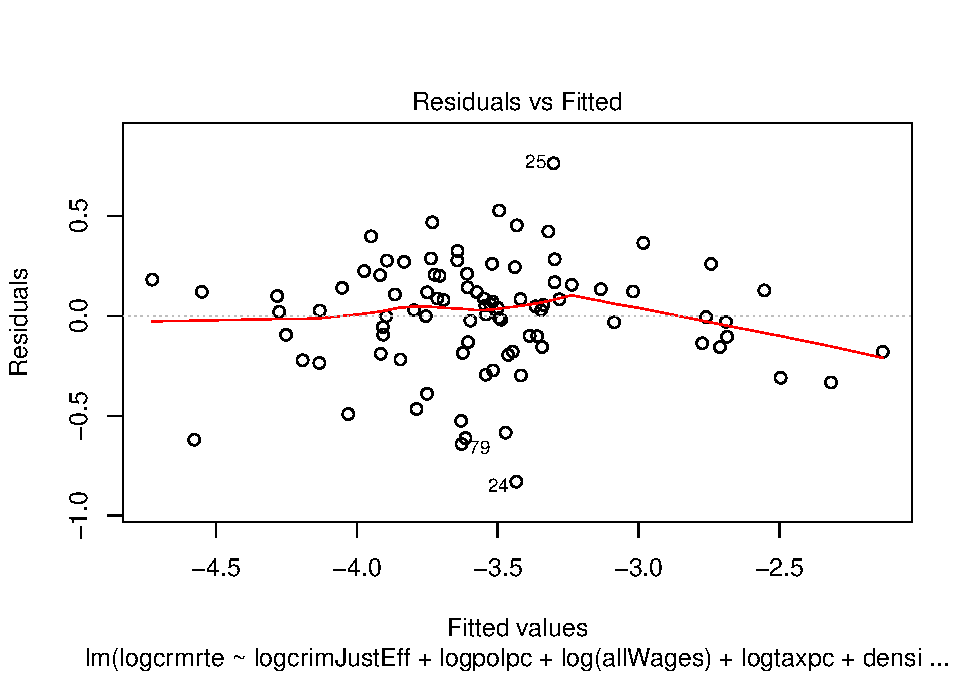
\includegraphics{Bagnard_Gaustad_Hartman_Leung_Lab_3_files/figure-latex/unnamed-chunk-100-1.pdf}
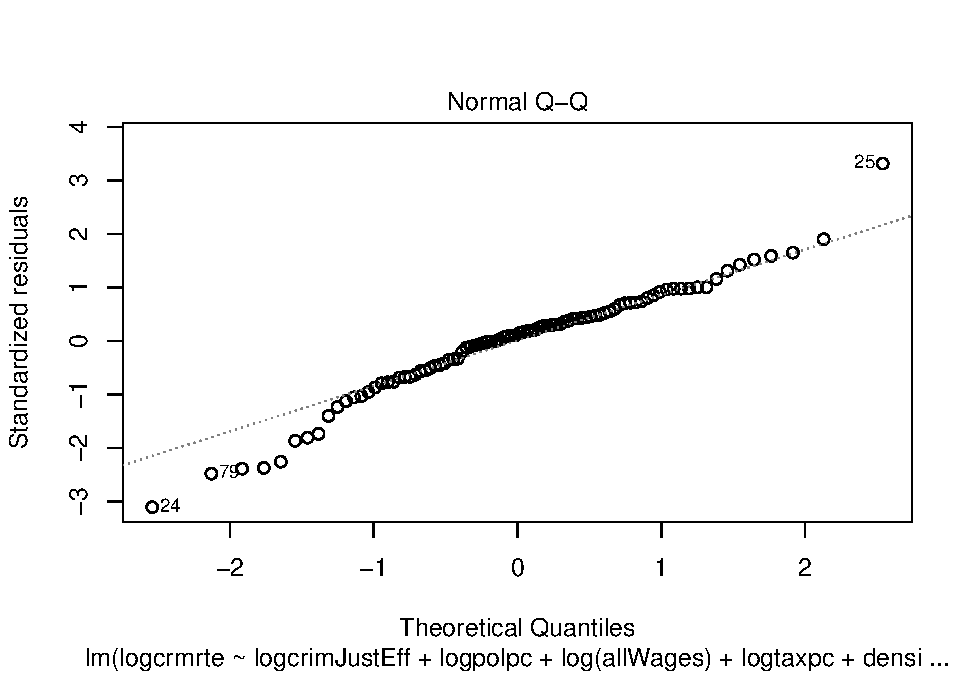
\includegraphics{Bagnard_Gaustad_Hartman_Leung_Lab_3_files/figure-latex/unnamed-chunk-100-2.pdf}
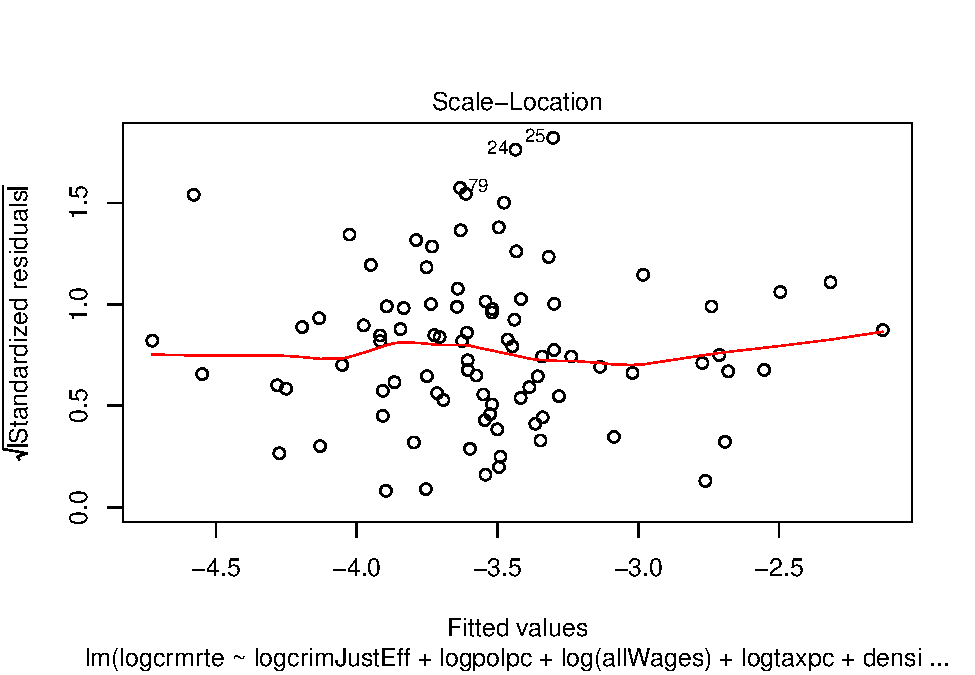
\includegraphics{Bagnard_Gaustad_Hartman_Leung_Lab_3_files/figure-latex/unnamed-chunk-100-3.pdf}
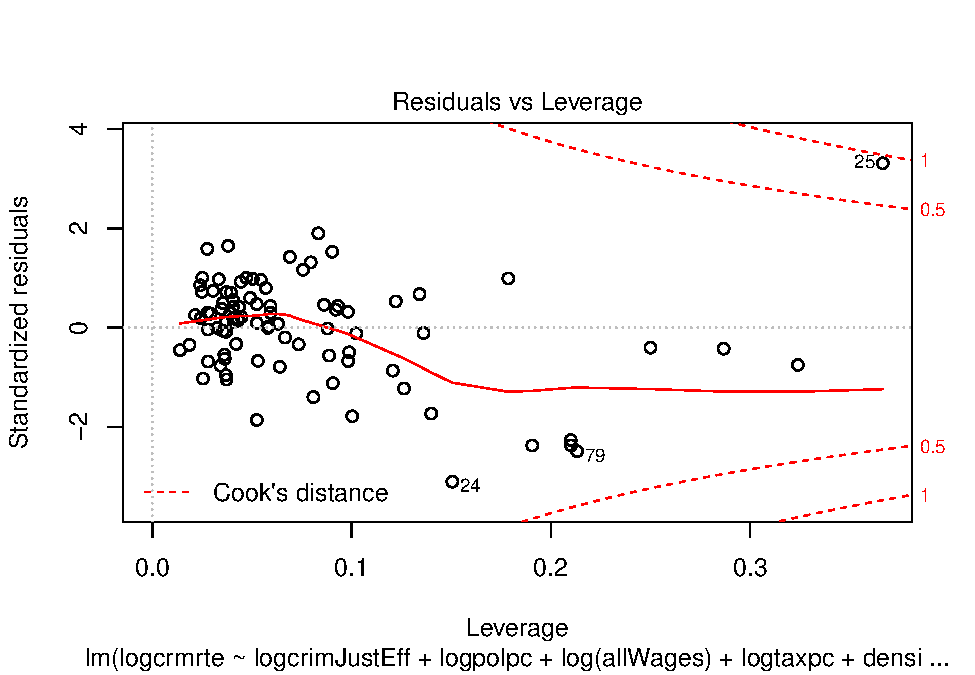
\includegraphics{Bagnard_Gaustad_Hartman_Leung_Lab_3_files/figure-latex/unnamed-chunk-100-4.pdf}
\textbf{Model 3 CLM Assumptions:}

\begin{itemize}
\item
  \textbf{MLR1 and 2}: Discussed earlier.
\item
  \textbf{MLR3} No perfect multicollinearity: We demonstrate that our
  independent variables are not perfectly multicolinear using the VIF
  function, and note that all of our variance inflation factors are less
  than 5.
\end{itemize}

\begin{Shaded}
\begin{Highlighting}[]
\KeywordTok{vif}\NormalTok{(model3)}
\end{Highlighting}
\end{Shaded}

\begin{verbatim}
## logcrimJustEff       logpolpc  log(allWages)       logtaxpc        density 
##       1.396993       1.594246       1.804483       1.400223       2.153101 
##    logpctmin80 
##       1.074812
\end{verbatim}

\begin{itemize}
\tightlist
\item
  \textbf{MLR4'} Zero Conditional Mean: From the residual vs.~fitted
  chart below, we see that the mean of the residuals mostly lie along 0,
  except towards the left side of our chart where there are fewer data
  points. We can reasonably conclude that we satisfy MLR4.
\end{itemize}

\begin{Shaded}
\begin{Highlighting}[]
\KeywordTok{plot}\NormalTok{(model3, }\DataTypeTok{which =} \DecValTok{1}\NormalTok{)}
\end{Highlighting}
\end{Shaded}

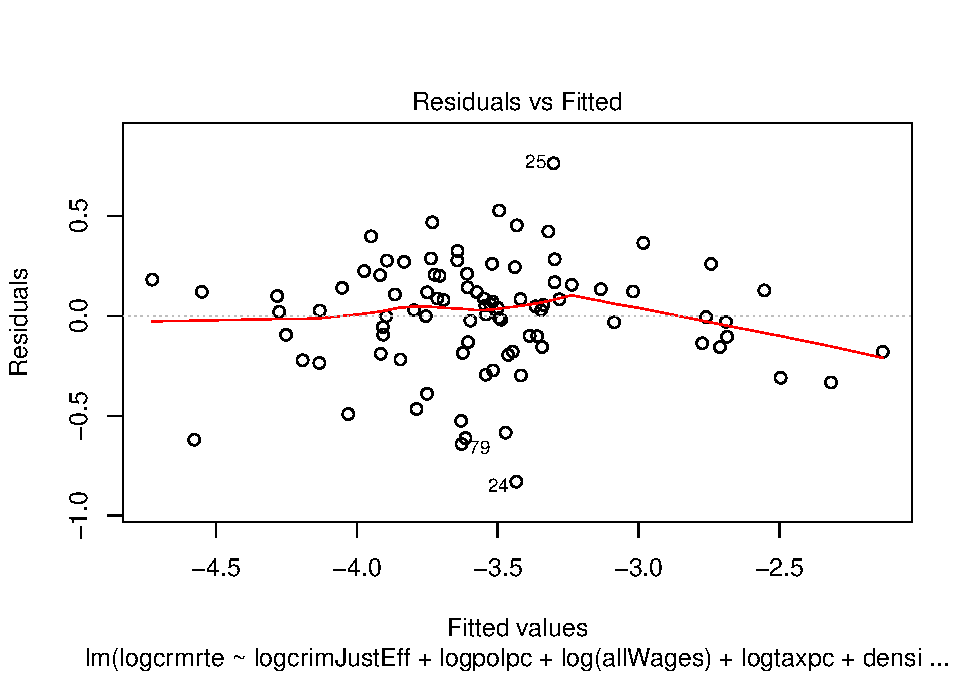
\includegraphics{Bagnard_Gaustad_Hartman_Leung_Lab_3_files/figure-latex/unnamed-chunk-102-1.pdf}

\begin{itemize}
\tightlist
\item
  \textbf{MLR5'} Spherical errors: We note from the residuals vs fitted
  chart above that we have some evidence of heteroscedasticity, since
  there are less datapoints on both the left and right of the chart. As
  a result, we use the vcovHC method to estimate a robust
  variance-covariance matrix using White and Huber's method and generate
  coefficients that are robust to heteroscedasticity.
\end{itemize}

\begin{Shaded}
\begin{Highlighting}[]
\KeywordTok{coeftest}\NormalTok{(model3, }\DataTypeTok{vcov=}\NormalTok{vcovHC)}
\end{Highlighting}
\end{Shaded}

\begin{verbatim}

t test of coefficients:

                Estimate Std. Error t value  Pr(>|t|)    
(Intercept)    -8.853835   5.824968 -1.5200   0.13232    
logcrimJustEff -0.425103   0.099585 -4.2687 5.193e-05 ***
logpolpc        0.340291   0.205883  1.6528   0.10214    
log(allWages)   0.919246   0.621673  1.4787   0.14302    
logtaxpc       -0.104223   0.290722 -0.3585   0.72088    
density         0.079268   0.040630  1.9510   0.05443 .  
logpctmin80     0.259682   0.046432  5.5928 2.792e-07 ***
---
Signif. codes:  0 '***' 0.001 '**' 0.01 '*' 0.05 '.' 0.1 ' ' 1
\end{verbatim}

\begin{itemize}
\tightlist
\item
  \textbf{MLR6'} Normality of errors: From the histogram below, we see
  that the residuals in our model follow a fairly normal distribution.
  In addition, since we have a large sample size of 90 datapoints, we
  can rely on a version of the central limit theorem to assume normally
  distributed errors.
\end{itemize}

\begin{Shaded}
\begin{Highlighting}[]
\KeywordTok{hist}\NormalTok{(model3}\OperatorTok{$}\NormalTok{residuals)}
\end{Highlighting}
\end{Shaded}

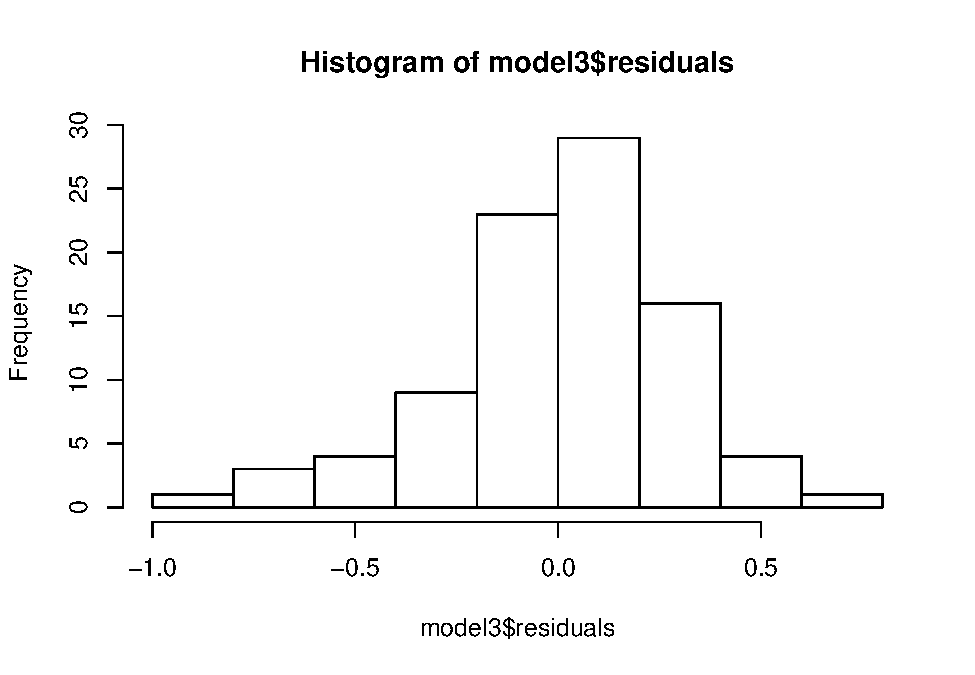
\includegraphics{Bagnard_Gaustad_Hartman_Leung_Lab_3_files/figure-latex/unnamed-chunk-104-1.pdf}

By satisfying these assumptions, we can expect that our coefficients are
approaching the true parameter values in probability.

\begin{Shaded}
\begin{Highlighting}[]
\KeywordTok{plot}\NormalTok{(model3)}
\end{Highlighting}
\end{Shaded}

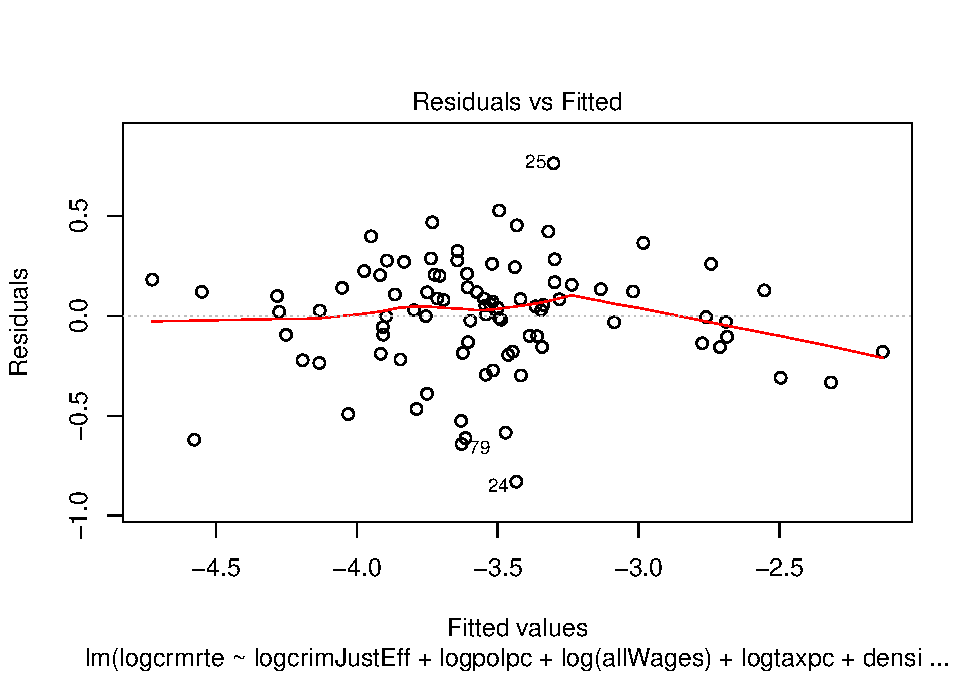
\includegraphics{Bagnard_Gaustad_Hartman_Leung_Lab_3_files/figure-latex/unnamed-chunk-105-1.pdf}
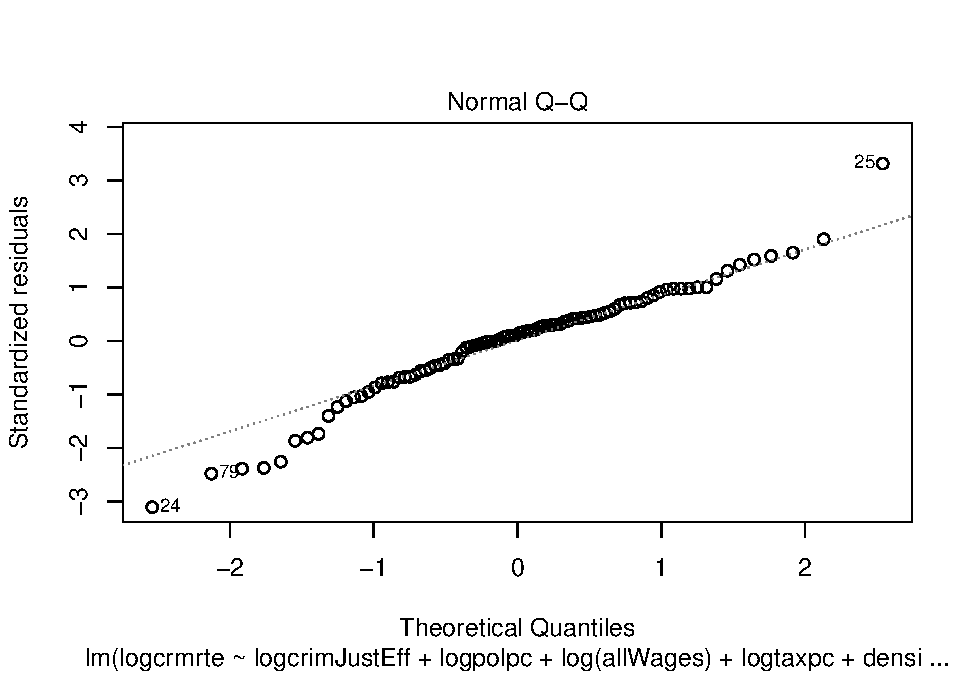
\includegraphics{Bagnard_Gaustad_Hartman_Leung_Lab_3_files/figure-latex/unnamed-chunk-105-2.pdf}
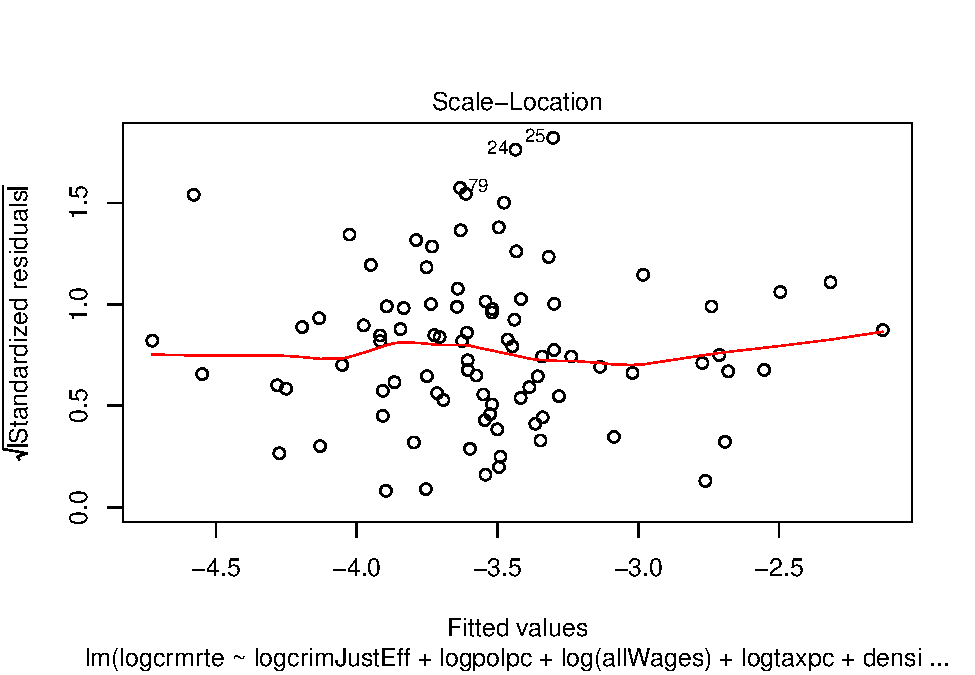
\includegraphics{Bagnard_Gaustad_Hartman_Leung_Lab_3_files/figure-latex/unnamed-chunk-105-3.pdf}
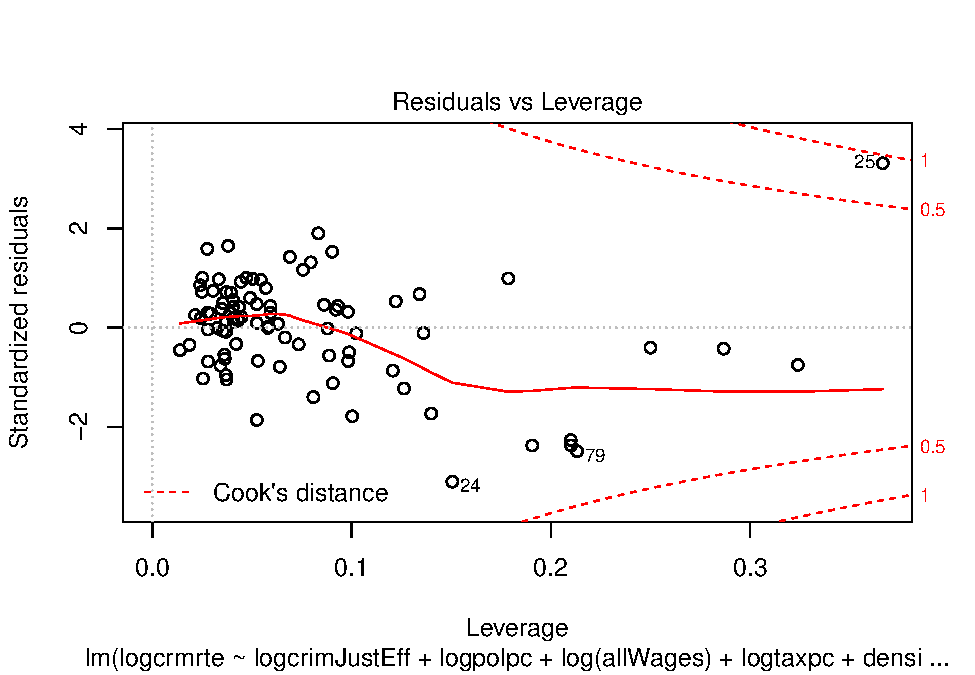
\includegraphics{Bagnard_Gaustad_Hartman_Leung_Lab_3_files/figure-latex/unnamed-chunk-105-4.pdf}

\hypertarget{analysis-to-be-updated}{%
\subsubsection{Analysis {[}TO BE
UPDATED{]}}\label{analysis-to-be-updated}}

The model shows a good fit, with an adjusted R-squared of 0.7322,
meaning that the model explains 73\% of the variation in crime.

For all of our 6 different independent variables, we note each of them
have statistical significance at the 95\% level or better. Of these 6,
criminal justice efficiency, minority percentages and density are the
most significant.

\textbf{Interpretation of coefficients (Assuming ceterus paribus):}

Positive coefficients: * Police presence: If we increase police per
capita by 1 unit, we expect the crime rate to increase by 33\%. *
AllWages: If we increase wages by 1 dollar, we expect the crime rate to
increase by 0.01\% * Density: If we increase density by 1 unit, we
expect the crime rate to increase by 5\% * Percentage of minorities: If
the percentage of minorities increase by 1\%, we expect the crime rate
to increase by 0.24\%

Negative coefficients: * Criminal justice efficiency: If we increase the
criminal justice efficiency by 1\%, we expect the crime rate to decrease
by 0.34\%. * Tax per capita: If we increase tax per capita by 1 unit, we
expect the crime rate to decrease by 0.35\%

In addition, the F-statistic is 40.04 with a statistically significant
p-value of \textless{} 2.2e-11. As a result, we reject the null
hypothesis that none of the independent variables help to describe
log(crmrate).

In the Residuals vs Leverage plot below, all the points have a cook's
distance of less than 0.5. While there is a point with 0.6 leverage,
there are no points that have residual that greatly alter the model
coefficients.

The root of standardized residuals all fall within about 1.6. This is
very good, as we can expect 95\% of the points to fall within 3
standardized residuals of each other. ( (⎯⎯√3)≈1.73 )

Finally, the residuals vs fitted plot shows a well centered and mostly
normal distribution about 0. There are no major trends or variation
changes across the fitted values. This suggests that major uncorrelated
variables have not been left out of the model.

\hypertarget{results}{%
\subsubsection{Results:}\label{results}}

\hypertarget{comparison-of-regression-models}{%
\subsection{Comparison of Regression
Models}\label{comparison-of-regression-models}}

*\textbf{Can anyone figure out why logcrimJustEff is on 2 lines?}

\begin{Shaded}
\begin{Highlighting}[]
\KeywordTok{stargazer}\NormalTok{(mod1,model2,model3,}\DataTypeTok{type=}\StringTok{"text"}\NormalTok{)}
\end{Highlighting}
\end{Shaded}

\begin{verbatim}

========================================================================================
                                            Dependent variable:                         
                    --------------------------------------------------------------------
                          logcrmrte                          logcrmrte                  
                             (1)                    (2)                    (3)          
----------------------------------------------------------------------------------------
unweighted_avg_wage        0.005***                                                     
                           (0.001)                                                      
                                                                                        
logcrimJustEff            -0.489***                                                     
                           (0.078)                                                      
                                                                                        
logcrimJustEff                                   -0.300***              -0.425***       
                                                  (0.082)                (0.064)        
                                                                                        
logpolpc                                           0.236                 0.340***       
                                                  (0.152)                (0.119)        
                                                                                        
log(allWages)                                      0.186                 0.919**        
                                                  (0.512)                (0.382)        
                                                                                        
logtaxpc                                           0.123                  -0.104        
                                                  (0.170)                (0.137)        
                                                                                        
density)                                          0.478***                              
                                                  (0.123)                               
                                                                                        
density                                                                  0.079***       
                                                                         (0.030)        
                                                                                        
logpctmin80                                                              0.260***       
                                                                         (0.033)        
                                                                                        
Constant                  -6.285***                -5.085                -8.854**       
                           (0.396)                (4.386)                (3.375)        
                                                                                        
----------------------------------------------------------------------------------------
Observations                  90                     90                     90          
R2                          0.459                  0.575                  0.740         
Adjusted R2                 0.447                  0.550                  0.722         
Residual Std. Error    0.408 (df = 87)        0.368 (df = 84)        0.289 (df = 83)    
F Statistic         36.949*** (df = 2; 87) 22.750*** (df = 5; 84) 39.465*** (df = 6; 83)
========================================================================================
Note:                                                        *p<0.1; **p<0.05; ***p<0.01
\end{verbatim}

Comparing the 3 models, we see that our adjusted R2 value has steadily
increased from 0.456-0.732 as we introduce more covariates which
indicates that we were able to explain more variation in our model not
purely by increasing the number of indepedent variables.

At the same time, our standard errors have decreased \textbf{insert more
commentary on standard errors}.

We see that by expanding our definitions of criminal justice efficiency
and economic opportunity between model 1 and model 3 lowered the
coefficients for logcrimJustEff and allWages. This is most likely
because that we were able to better explain the effects with our newer
variables.

Comment on practical significance after week 12

\hypertarget{conclusion}{%
\section{Conclusion}\label{conclusion}}

\hypertarget{policy-recommendations}{%
\subsection{Policy Recommendations}\label{policy-recommendations}}

Given that across all 3 models, we show that both criminal justice
efficiency and tax revenues per capita have negative correlations to
crime rate, we propose the policy recommendations below to address these
issues. In addition, since minority percentages and density were found
to be highly significant in the model 3, we believe our recommendations
will be of particularly help to those running for political office in
counties with a high percentage of minorities or dense urban
populations.

\begin{enumerate}
\def\labelenumi{\arabic{enumi}.}
\item
  Since increasing both criminal justice and tax revenues are negatively
  correlated, we propose providing more funding for the local justice
  system.
\item
  While increasing taxes on constituents may be difficult politically
  and may cost candidates the ballot, candidates can instead try to
  attract investment to bring more jobs with higher wages so you can
  increase revenues.
\item
  Candidates can also propose to levy taxes on things that could lead to
  crimes or violence such as alcohol and weapons.
\item
  Given the significance and relatively large coefficient size of
  percentage minority, candidates should enroll local law enforcement
  into bias training.
\end{enumerate}

\hypertarget{ommitted-variables}{%
\subsection{Ommitted Variables}\label{ommitted-variables}}

\begin{longtable}[]{@{}l@{}}
\toprule
Expected correlation between omitted and included
variables\tabularnewline
\midrule
\endhead
\bottomrule
\end{longtable}

\begin{longtable}[]{@{}llll@{}}
\toprule
\begin{minipage}[b]{0.18\columnwidth}\raggedright
Omitted Variable\strut
\end{minipage} & \begin{minipage}[b]{0.19\columnwidth}\raggedright
Crime Rate (\(B_k\))\strut
\end{minipage} & \begin{minipage}[b]{0.31\columnwidth}\raggedright
Criminal Justice Effectiveness\strut
\end{minipage} & \begin{minipage}[b]{0.20\columnwidth}\raggedright
Economic Conditions\strut
\end{minipage}\tabularnewline
\midrule
\endhead
\begin{minipage}[t]{0.18\columnwidth}\raggedright
Education\strut
\end{minipage} & \begin{minipage}[t]{0.19\columnwidth}\raggedright
-\strut
\end{minipage} & \begin{minipage}[t]{0.31\columnwidth}\raggedright
unknown\strut
\end{minipage} & \begin{minipage}[t]{0.20\columnwidth}\raggedright
+\strut
\end{minipage}\tabularnewline
\begin{minipage}[t]{0.18\columnwidth}\raggedright
Social Services\strut
\end{minipage} & \begin{minipage}[t]{0.19\columnwidth}\raggedright
-\strut
\end{minipage} & \begin{minipage}[t]{0.31\columnwidth}\raggedright
unknown\strut
\end{minipage} & \begin{minipage}[t]{0.20\columnwidth}\raggedright
unknown\strut
\end{minipage}\tabularnewline
\begin{minipage}[t]{0.18\columnwidth}\raggedright
Unemployment\strut
\end{minipage} & \begin{minipage}[t]{0.19\columnwidth}\raggedright
+\strut
\end{minipage} & \begin{minipage}[t]{0.31\columnwidth}\raggedright
unknown\strut
\end{minipage} & \begin{minipage}[t]{0.20\columnwidth}\raggedright
-\strut
\end{minipage}\tabularnewline
\begin{minipage}[t]{0.18\columnwidth}\raggedright
Gang Activity\strut
\end{minipage} & \begin{minipage}[t]{0.19\columnwidth}\raggedright
+\strut
\end{minipage} & \begin{minipage}[t]{0.31\columnwidth}\raggedright
-\strut
\end{minipage} & \begin{minipage}[t]{0.20\columnwidth}\raggedright
-\strut
\end{minipage}\tabularnewline
\bottomrule
\end{longtable}

The 4 major identified ommited variables are shown above.

\begin{itemize}
\tightlist
\item
  Education is an important variable because of demographic insights it
  provides. First, adults with higher education are less likely to
  participate in Crime and are more likely to have better economic
  opportunity. Second, a strong school system is also likely correlated
  with less youth crime. Because of these expected correlations we are
  likely overestimating the economic conditions coefficient estimate.
\item
  Available Social Services could also lower crime. Citizens with strong
  social services support have more options to get help when they lack
  means for purchasing basic life needs. However this is more difficult
  to predict, as some social service projects, like homeless shelters,
  could lead to more criminal activity.
\item
  Unemployment is used as an important indicator of economic health and
  opportunity. This is would be highly correlated to economic conditions
  variables like sum of wages. This indicator variable if added to the
  model would decrease the magnitude of the sum of wage means
  coefficient estimate.\\
\item
  Gang or Organized Crime is special case of crime that contains unique
  causes. It is expected that it would be negatively correlated with
  criminal justice effectiveness as large social pressures prevent
  witnesses from supporting prosecution. Gang crime is also negatively
  correlated with economic conditions. From these assumed correlations,
  we can say that criminal justice effectiveness and economic conditions
  are both underestimated compared to including gang activity
  operationalized variable in the model.
\end{itemize}

\hypertarget{research-recommendations}{%
\subsection{Research Recommendations}\label{research-recommendations}}

We have shown in this report 3 different models that seek to explain and
model changes in the crime rate in North Carolina in 1980. We start with
the fundamental premise that crime is caused by both criminal justice
efficiency and economic conditions, and further develop our definition
of these two key explanatory variables which each new model.

In Model 3, we were able to explain up to 73\% of the variation in our
data, and found statistical significance at the 95\% level or better for
each of our covariates. Of these, we believe that increasing the
efficiency of the criminal justice system and tax revenues were the most
important, particularly for counties with high density and minority
populations. However, our findings should be noted with caution as we
were unable to study the effect of several ommitted variables including
education, availability of social services, unemployment rates and the
presence of organized crime. Had we been able to collect data on these
variables and apply them in our model, we believe we could increase
accuracy without bias.

\hypertarget{appendix}{%
\section{Appendix}\label{appendix}}

\begin{Shaded}
\begin{Highlighting}[]
\KeywordTok{options}\NormalTok{(}\DataTypeTok{repr.plot.width=}\DecValTok{8}\NormalTok{, }\DataTypeTok{repr.plot.height=}\DecValTok{4}\NormalTok{)}
\CommentTok{#myData<-myData[, c("crmrte", "prbarr", "prbconv", "prbpris", "avgsen", "polpc", "density", "taxpc",}
\CommentTok{#           "pctmin80", "wcon", "wtuc", "wtrd", "wfir", "wser", "wmfg", "wfed", "wsta", "wloc",}
\CommentTok{#           "mix", "pctymle")]}
\NormalTok{myData<-dfCrime }\OperatorTok\StringTok{ }\KeywordTok{filter}\NormalTok{(other}\OperatorTok{==}\DecValTok{1}\NormalTok{)}
\NormalTok{myData<-myData[, }\KeywordTok{c}\NormalTok{(}\StringTok{"logcrmrte"}\NormalTok{, }\StringTok{"logprbarr"}\NormalTok{, }\StringTok{"logprbconv"}\NormalTok{, }\StringTok{"logprbpris"}\NormalTok{, }\StringTok{"logavgsen"}\NormalTok{, }\StringTok{"logpolpc"}\NormalTok{, }\StringTok{"logtaxpc"}\NormalTok{,}
           \StringTok{"logpctmin80"}\NormalTok{, }\StringTok{"logwcon"}\NormalTok{, }\StringTok{"logwtuc"}\NormalTok{, }\StringTok{"logwtrd"}\NormalTok{, }\StringTok{"logwfir"}\NormalTok{, }\StringTok{"logwser"}\NormalTok{, }\StringTok{"logwmfg"}\NormalTok{, }\StringTok{"logwfed"}\NormalTok{, }\StringTok{"logwsta"}\NormalTok{, }\StringTok{"logwloc"}\NormalTok{,}
           \StringTok{"logmix"}\NormalTok{, }\StringTok{"logpctymle"}\NormalTok{)]}
\NormalTok{r0 <-}\StringTok{ }\NormalTok{myData }\OperatorTok\StringTok{ }\KeywordTok{correlate}\NormalTok{() }\OperatorTok\StringTok{ }\KeywordTok{network_plot}\NormalTok{(}\DataTypeTok{min_cor=}\NormalTok{.}\DecValTok{25}\NormalTok{)}
\end{Highlighting}
\end{Shaded}

\begin{verbatim}

Correlation method: 'pearson'
Missing treated using: 'pairwise.complete.obs'
\end{verbatim}

\begin{Shaded}
\begin{Highlighting}[]
\NormalTok{myData<-dfCrime }\OperatorTok\StringTok{ }\KeywordTok{filter}\NormalTok{(central}\OperatorTok{==}\DecValTok{1}\NormalTok{)}
\NormalTok{myData<-myData[, }\KeywordTok{c}\NormalTok{(}\StringTok{"logcrmrte"}\NormalTok{, }\StringTok{"logprbarr"}\NormalTok{, }\StringTok{"logprbconv"}\NormalTok{, }\StringTok{"logprbpris"}\NormalTok{, }\StringTok{"logavgsen"}\NormalTok{, }\StringTok{"logpolpc"}\NormalTok{, }\StringTok{"logtaxpc"}\NormalTok{,}
           \StringTok{"logpctmin80"}\NormalTok{, }\StringTok{"logwcon"}\NormalTok{, }\StringTok{"logwtuc"}\NormalTok{, }\StringTok{"logwtrd"}\NormalTok{, }\StringTok{"logwfir"}\NormalTok{, }\StringTok{"logwser"}\NormalTok{, }\StringTok{"logwmfg"}\NormalTok{, }\StringTok{"logwfed"}\NormalTok{, }\StringTok{"logwsta"}\NormalTok{, }\StringTok{"logwloc"}\NormalTok{,}
           \StringTok{"logmix"}\NormalTok{, }\StringTok{"logpctymle"}\NormalTok{)]}
\NormalTok{r1 <-}\StringTok{ }\NormalTok{myData }\OperatorTok\StringTok{ }\KeywordTok{correlate}\NormalTok{() }\OperatorTok\StringTok{ }\KeywordTok{network_plot}\NormalTok{(}\DataTypeTok{min_cor=}\NormalTok{.}\DecValTok{25}\NormalTok{)}
\end{Highlighting}
\end{Shaded}

\begin{verbatim}

Correlation method: 'pearson'
Missing treated using: 'pairwise.complete.obs'
\end{verbatim}

\begin{Shaded}
\begin{Highlighting}[]
\NormalTok{myData<-dfCrime }\OperatorTok\StringTok{ }\KeywordTok{filter}\NormalTok{(west}\OperatorTok{==}\DecValTok{1}\NormalTok{)}
\NormalTok{myData<-myData[, }\KeywordTok{c}\NormalTok{(}\StringTok{"logcrmrte"}\NormalTok{, }\StringTok{"logprbarr"}\NormalTok{, }\StringTok{"logprbconv"}\NormalTok{, }\StringTok{"logprbpris"}\NormalTok{, }\StringTok{"logavgsen"}\NormalTok{, }\StringTok{"logpolpc"}\NormalTok{, }\StringTok{"logtaxpc"}\NormalTok{,}
           \StringTok{"logpctmin80"}\NormalTok{, }\StringTok{"logwcon"}\NormalTok{, }\StringTok{"logwtuc"}\NormalTok{, }\StringTok{"logwtrd"}\NormalTok{, }\StringTok{"logwfir"}\NormalTok{, }\StringTok{"logwser"}\NormalTok{, }\StringTok{"logwmfg"}\NormalTok{, }\StringTok{"logwfed"}\NormalTok{, }\StringTok{"logwsta"}\NormalTok{, }\StringTok{"logwloc"}\NormalTok{,}
           \StringTok{"logmix"}\NormalTok{, }\StringTok{"logpctymle"}\NormalTok{)]}
\NormalTok{r2 <-}\StringTok{ }\NormalTok{myData }\OperatorTok\StringTok{ }\KeywordTok{correlate}\NormalTok{() }\OperatorTok\StringTok{ }\KeywordTok{network_plot}\NormalTok{(}\DataTypeTok{min_cor=}\NormalTok{.}\DecValTok{25}\NormalTok{)}
\end{Highlighting}
\end{Shaded}

\begin{verbatim}

Correlation method: 'pearson'
Missing treated using: 'pairwise.complete.obs'
\end{verbatim}

\begin{Shaded}
\begin{Highlighting}[]
\KeywordTok{grid.arrange}\NormalTok{(}\KeywordTok{arrangeGrob}\NormalTok{(r1, }\DataTypeTok{bottom =} \StringTok{'Central Region Correlation Plot'}\NormalTok{), }\DataTypeTok{ncol=}\DecValTok{1}\NormalTok{)}
\end{Highlighting}
\end{Shaded}

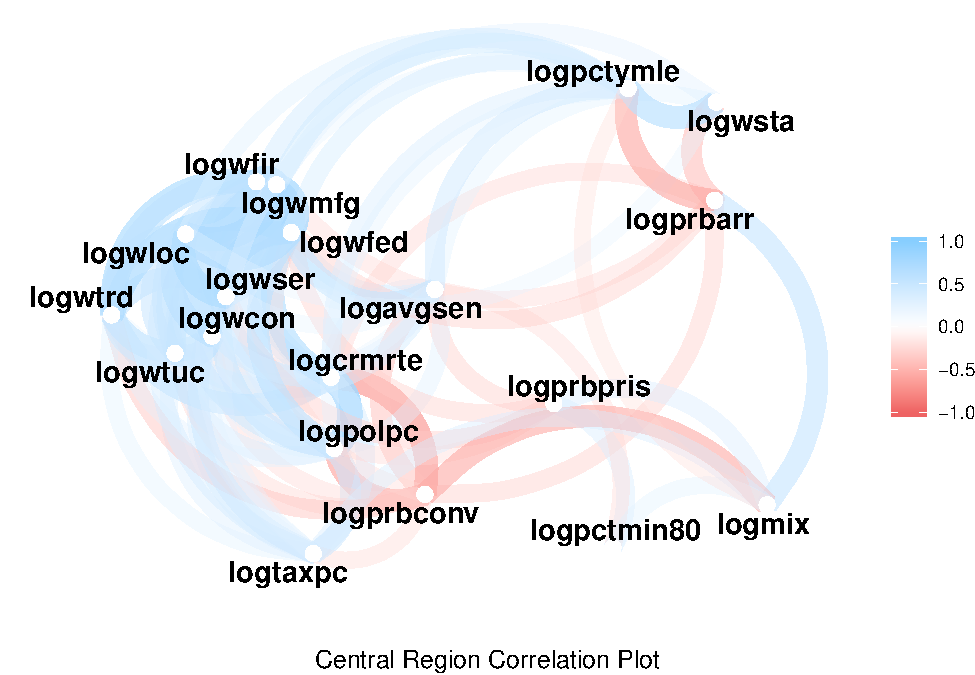
\includegraphics{Bagnard_Gaustad_Hartman_Leung_Lab_3_files/figure-latex/unnamed-chunk-107-1.pdf}

\begin{Shaded}
\begin{Highlighting}[]
\KeywordTok{grid.arrange}\NormalTok{(}\KeywordTok{arrangeGrob}\NormalTok{(r2, }\DataTypeTok{bottom =} \StringTok{'Western Region Correlation Plot'}\NormalTok{), }\DataTypeTok{ncol=}\DecValTok{1}\NormalTok{)}
\end{Highlighting}
\end{Shaded}

\includegraphics{Bagnard_Gaustad_Hartman_Leung_Lab_3_files/figure-latex/unnamed-chunk-107-2.pdf}

\begin{Shaded}
\begin{Highlighting}[]
\KeywordTok{grid.arrange}\NormalTok{(}\KeywordTok{arrangeGrob}\NormalTok{(r0, }\DataTypeTok{bottom =} \StringTok{'Other Region Correlation Plot'}\NormalTok{), }\DataTypeTok{ncol=}\DecValTok{1}\NormalTok{)}
\end{Highlighting}
\end{Shaded}

\includegraphics{Bagnard_Gaustad_Hartman_Leung_Lab_3_files/figure-latex/unnamed-chunk-107-3.pdf}

\begin{Shaded}
\begin{Highlighting}[]
\NormalTok{myData<-dfCrime }\OperatorTok\StringTok{ }\KeywordTok{filter}\NormalTok{(urban}\OperatorTok{==}\DecValTok{0}\NormalTok{)}
\NormalTok{myData<-myData[, }\KeywordTok{c}\NormalTok{(}\StringTok{"logcrmrte"}\NormalTok{, }\StringTok{"logprbarr"}\NormalTok{, }\StringTok{"logprbconv"}\NormalTok{, }\StringTok{"logprbpris"}\NormalTok{, }\StringTok{"logavgsen"}\NormalTok{, }\StringTok{"logpolpc"}\NormalTok{, }\StringTok{"logtaxpc"}\NormalTok{,}
           \StringTok{"logpctmin80"}\NormalTok{, }\StringTok{"logwcon"}\NormalTok{, }\StringTok{"logwtuc"}\NormalTok{, }\StringTok{"logwtrd"}\NormalTok{, }\StringTok{"logwfir"}\NormalTok{, }\StringTok{"logwser"}\NormalTok{, }\StringTok{"logwmfg"}\NormalTok{, }\StringTok{"logwfed"}\NormalTok{, }\StringTok{"logwsta"}\NormalTok{, }\StringTok{"logwloc"}\NormalTok{,}
           \StringTok{"logmix"}\NormalTok{, }\StringTok{"logpctymle"}\NormalTok{)]}
\NormalTok{r0 <-}\StringTok{ }\NormalTok{myData }\OperatorTok\StringTok{ }\KeywordTok{correlate}\NormalTok{() }\OperatorTok\StringTok{ }\KeywordTok{network_plot}\NormalTok{(}\DataTypeTok{min_cor=}\NormalTok{.}\DecValTok{25}\NormalTok{)}
\end{Highlighting}
\end{Shaded}

\begin{verbatim}

Correlation method: 'pearson'
Missing treated using: 'pairwise.complete.obs'
\end{verbatim}

\begin{Shaded}
\begin{Highlighting}[]
\NormalTok{myData<-dfCrime }\OperatorTok\StringTok{ }\KeywordTok{filter}\NormalTok{(urban}\OperatorTok{==}\DecValTok{1}\NormalTok{)}
\NormalTok{myData<-myData[, }\KeywordTok{c}\NormalTok{(}\StringTok{"logcrmrte"}\NormalTok{, }\StringTok{"logprbarr"}\NormalTok{, }\StringTok{"logprbconv"}\NormalTok{, }\StringTok{"logprbpris"}\NormalTok{, }\StringTok{"logavgsen"}\NormalTok{, }\StringTok{"logpolpc"}\NormalTok{,  }\StringTok{"logtaxpc"}\NormalTok{,}
           \StringTok{"logpctmin80"}\NormalTok{, }\StringTok{"logwcon"}\NormalTok{, }\StringTok{"logwtuc"}\NormalTok{, }\StringTok{"logwtrd"}\NormalTok{, }\StringTok{"logwfir"}\NormalTok{, }\StringTok{"logwser"}\NormalTok{, }\StringTok{"logwmfg"}\NormalTok{, }\StringTok{"logwfed"}\NormalTok{, }\StringTok{"logwsta"}\NormalTok{, }\StringTok{"logwloc"}\NormalTok{,}
           \StringTok{"logmix"}\NormalTok{, }\StringTok{"logpctymle"}\NormalTok{)]}
\NormalTok{r1 <-}\StringTok{ }\NormalTok{myData }\OperatorTok\StringTok{ }\KeywordTok{correlate}\NormalTok{() }\OperatorTok\StringTok{ }\KeywordTok{network_plot}\NormalTok{(}\DataTypeTok{min_cor=}\NormalTok{.}\DecValTok{25}\NormalTok{)}
\end{Highlighting}
\end{Shaded}

\begin{verbatim}

Correlation method: 'pearson'
Missing treated using: 'pairwise.complete.obs'
\end{verbatim}

\begin{Shaded}
\begin{Highlighting}[]
\KeywordTok{grid.arrange}\NormalTok{(}\KeywordTok{arrangeGrob}\NormalTok{(r0, }\DataTypeTok{bottom =} \StringTok{'Non-Urban Correlation Plot'}\NormalTok{), }\DataTypeTok{ncol=}\DecValTok{1}\NormalTok{)}
\end{Highlighting}
\end{Shaded}

\includegraphics{Bagnard_Gaustad_Hartman_Leung_Lab_3_files/figure-latex/unnamed-chunk-107-4.pdf}

\begin{Shaded}
\begin{Highlighting}[]
\KeywordTok{grid.arrange}\NormalTok{(}\KeywordTok{arrangeGrob}\NormalTok{(r1, }\DataTypeTok{bottom =} \StringTok{'Urban Correlation Plot'}\NormalTok{), }\DataTypeTok{ncol=}\DecValTok{1}\NormalTok{)}
\end{Highlighting}
\end{Shaded}

\includegraphics{Bagnard_Gaustad_Hartman_Leung_Lab_3_files/figure-latex/unnamed-chunk-107-5.pdf}


\end{document}
